\documentclass{iutbscthesis}
\usepackage{kantlipsum} % This package is used to generate place holder text. Remove it in the actual world.

\tolerance=1 % Allow some flexibility for line breaking
\emergencystretch=\maxdimen % Allow line breaking to stretch a little more
\hyphenpenalty=10000 % Allow hyphenation with a reasonable penalty
\hbadness=10000 % Suppress most warnings about underfull or overfull lines

% The iutbscthesis uses biblatex for bibliography management.
% You can learn the basics of biblatex from:
% https://www.overleaf.com/learn/latex/Bibliography_management_with_biblatex
\addbibresource{citations.bib}
\graphicspath{{./figures/}}
\DeclareGraphicsExtensions{.pdf, .png, .jpg, .jpeg}


% The complete title of your thesis, mandatory
\title{\Large{Optimizing CAM Refinement with Swin-based Feature Affinity for Weakly Supervised Semantic Segmentation}}

% Use the \addauthor command to keep adding authors with student ID
\addauthor{Anika Farzana}{200041204}
\addauthor{K. M. Abesh Ahsan}{200041225}
\addauthor{Sayema Amin}{200041234}

% Use the \supervisor command to define the supervisor with name, designation, and department
% There needs to be one and only one supervisor
\supervisor{Dr. Hasanul Kabir}{Professor}{Department of Computer Science and Engineering}

% Use the \addcosupervisor command to add a cosupervisor. There might be no cosupervisor at all
% % In that case, just remove all of the \addcosupervisor commands.
% \addcosupervisor{Dr.\ Sue Permann}{Assistant Professor}{Department of Computer Science and Engineering}
% \addcosupervisor{Mr. Francis FullOfFrenchPeople}{Lecturer}{Department of Computer Science and Engineering}

% Complete department name, mandatory
\department{Department of Computer Science and Engineering}

% Complete program name, mandatory
\program{BACHELOR OF SCIENCE IN COMPUTER SCIENCE AND ENGINEERING}

% Date (day, month name, and year) when the presentation took place, mandatory
\defensedate{29}{April}{2025}

\begin{document}

%-------------------------- FRONT MATTER --------------------------%

% Generate cover page of the report to be printed on the hard cover
\coverpage

% Switch to roman page numbering
\pagenumbering{roman}

% Generate the title leaf, mandatory
\titlepage

% Auto generate declaration of candidate based on previous info, mandatory
\declarationofcandidate

% % Dedicate report to someone. You may add more sentences to it.
% \dedicatedto{our supervisor without whom this degree would have been completed six months earlier}

\tableofcontents
\listoffigures
\listoftables

\clearpage

% Add abbreviations within this environment using the \abbr command
% \begin{abbreviations}
%     \abbr{CNN}{Convolutional Neural Network}
%     \abbr{PIP}{PIP Installs Packages}
%     \abbr{TikZ}{TikZ ist kein Zeichenprogramm}
%     \abbr{WIKI}{What I Know Is}
% \end{abbreviations}

% Any acknowledgement that you want to write goes in the following environment

\begin{acknowledgement}
    I am profoundly grateful to my supervisor, Dr. Hasanul Kabir, Professor, Department of Computer Science and Engineering, for his outstanding guidance, support, and feedback throughout this research journey. His expertise and encouragement have been pivotal in shaping the direction and quality of this thesis.

His patience and dedication to his work have inspired me to aim for excellence and approach challenges with curiosity and determination. His constructive feedback and insightful suggestions have significantly deepened my understanding of the domain and inspired me to think critically and creatively.

It has been an honor to work under his supervision, and I deeply appreciate his invaluable time and effort in guiding me through this research.
\end{acknowledgement}

% Write your abstract here.
\begin{abstract}
Semantic segmentation is a key task in computer vision that involves interpreting images at the pixel level. While fully supervised methods provide high accuracy, they require extensive pixel-level annotations, making them resource-intensive. Weakly Supervised Semantic Segmentation (WSSS) addresses this issue by using weaker supervision formats like image-level labels, reducing the need for annotation while still training effective segmentation models.

Recent WSSS advancements have shown that competitive performance can be reached with minimal labeled data through the use of Class Activation Maps (CAMs). However, challenges such as sparsity and inadequate boundary delineation affect CAM quality.

This study aims to improve CAM quality by exploring effective backbone architectures and refinement strategies. We investigate multi-modal architectures like UniCL and hierarchical transformers such as Swin Transformer to enhance feature extraction. To further refine CAMs, we use an affinity-based framework that combines decoder-derived affinities with encoder affinity maps, creating more semantically coherent pseudo-labels. Additionally, a Pixel-Adaptive Refinement (PAR) module proposed by \cite{wsss_afa_affinity_from_attention} to refine pseudo-labels based on local similarities, ensuring better object boundaries.

Experiments on the PASCAL VOC 2012 dataset demonstrate that our approach achieves strong segmentation performance, with a mean IoU of 50.3\% on the validation set and 50.8\% on the test set. The model performs best on large, distinctive categories such as \textit{bus}, \textit{sheep}, and \textit{horse}, but struggles with small or underrepresented classes like \textit{person}, \textit{chair}, and \textit{potted plant}. The poor performance of the \textit{person} class arises from initial CAM confidence being biased toward background regions, which propagates through the Random Walk-based Refinement Module (RFM), while the Pixel-Adaptive module tends to oversmooth fine structures such as limbs. These challenges are further compounded by biases in UniCL’s pretraining datasets (ImageNet-21K and YFCC-14M), which provide limited representation for human-centric and small-object categories.

Overall, our findings highlight the effectiveness of UniCL and Swin Transformer in enhancing CAM quality and segmentation performance under weak supervision, while also revealing key limitations that motivate future work on scale-aware and bias-compensated refinement strategies.
\end{abstract}

%-------------------------- MAIN BODY --------------------------%
% Switch to arabic page numbering
\pagenumbering{arabic}

\chapter{Introduction}
\label{chap:introduction}

\section{Semantic Segmentation}
\label{sec:semantic_segmentation}
In recent years, the field of computer vision has undergone rapid advancements, largely driven by the increasing availability of large-scale annotated datasets, powerful computational resources, and deep learning architectures. Among the many tasks in computer vision, semantic segmentation has emerged as one of the most critical and challenging problems due to its potential applications in numerous real-world domains, such as autonomous driving, medical imaging, remote sensing, robotics, and augmented reality. Unlike simple image classification, which assigns a single label to an entire image, semantic segmentation aims to provide a pixel-level understanding of the visual scene by assigning a semantic label to every pixel in an image as shown in \autoref{fig:semantic_segmentation_example}. This process enables machines to perceive not just the presence of objects, but also their exact spatial extents and boundaries within the visual field.

\begin{figure}[htbp]
    \centering
    \setlength{\tabcolsep}{2pt} % adjust spacing
    \renewcommand{\arraystretch}{0.9}
    % \fbox{ % Add border around the figure
        \begin{minipage}{0.8\textwidth}
            \centering
            % CAMs with class labels on the left
            \begin{tabular}{c c} % first column = label

            % Column headers
            (a) Original Image & (b) Segmented Image \\
            [1mm]
            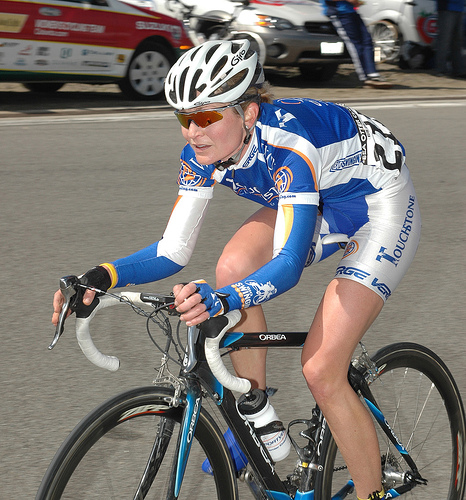
\includegraphics[width=0.45\textwidth,height=0.45\textwidth]{figures/originals/2011_002135.jpg}
            & 
            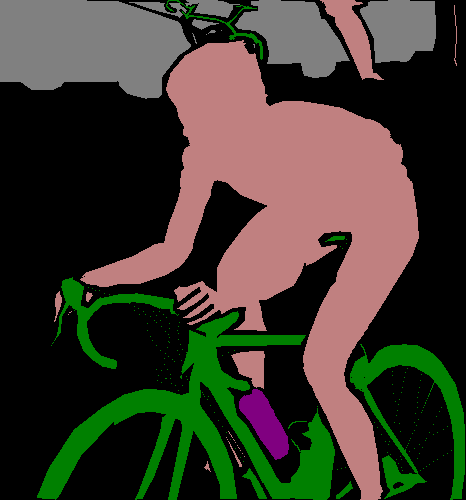
\includegraphics[width=0.45\textwidth,height=0.45\textwidth]{figures/colored_gts/2011_002135.png}
            \\
            \end{tabular}
        \end{minipage}
    % }
    \caption{Original image and Segmented Image.}
    \label{fig:semantic_segmentation_example}
\end{figure}

The goal of semantic segmentation is to transform raw visual data into structured and meaningful representations that align with human perception. For example, in an autonomous driving scenario, semantic segmentation allows a vehicle to distinguish between roads, pedestrians, vehicles, and traffic signs, ensuring both accurate decision-making and safety. In medical imaging, it aids in the precise delineation of organs, tissues, or pathological regions, thereby assisting in diagnosis and treatment planning. Such applications highlight the importance of fine-grained visual understanding, making semantic segmentation a cornerstone task for achieving scene comprehension in artificial intelligence systems.

Traditional approaches to semantic segmentation relied heavily on hand-crafted features and classical machine learning methods such as random forests, support vector machines (SVMs), and conditional random fields (CRFs). While these methods achieved moderate success on specific datasets, they were limited by their inability to capture complex spatial and contextual relationships in images. The breakthrough came with the advent of deep convolutional neural networks (CNNs), which revolutionized the field by automatically learning hierarchical feature representations from data. The introduction of architectures such as Fully Convolutional Networks (FCNs) marked a major milestone, replacing fully connected layers with convolutional ones to enable end-to-end pixel-level prediction. Subsequent models, including U-Net, SegNet, DeepLab, and PSPNet, have further refined this capability by incorporating multi-scale feature extraction, encoder-decoder designs, and attention mechanisms to enhance segmentation accuracy and robustness.

Despite these advances, semantic segmentation still faces several challenges. High-quality pixel-level annotations are expensive and time-consuming to obtain, especially for large datasets. Models must also handle issues such as class imbalance, occlusion, scale variation, and boundary precision, which can significantly affect performance. Furthermore, deep models typically require substantial computational resources, making real-time inference a major concern in resource-constrained environments such as mobile or embedded systems. Recent research has thus explored various directions to address these limitations, including weakly supervised, semi-supervised, and unsupervised approaches that reduce the dependency on dense annotations, as well as lightweight architectures optimized for speed and efficiency.

The increasing focus on semantic segmentation has also sparked interest in integrating it with other vision tasks, such as instance and panoptic segmentation, which aim to provide a more comprehensive understanding of the scene by distinguishing individual object instances. Additionally, combining segmentation with temporal and 3D information, as in video and point cloud segmentation, continues to push the boundaries of scene understanding beyond static 2D imagery.

In summary, semantic segmentation represents a vital step toward achieving full scene understanding in computer vision. By providing detailed, structured, and interpretable representations of visual data, it bridges the gap between low-level pixel information and high-level semantic concepts. This research report explores the principles, methodologies, and recent advancements in semantic segmentation, with particular emphasis on deep learning-based approaches and their applications. Furthermore, it discusses the current challenges and potential future directions that could lead to more efficient, generalizable, and human-like visual perception systems.


\subsection{Fully Supervised Semantic Segmentation}
\label{subsec:fully_supervised}
Fully supervised semantic segmentation represents the traditional and most widely adopted paradigm for training segmentation models. In this approach, models are trained on datasets that contain pixel-level annotations—where every pixel in each training image is manually labeled with its corresponding class. This allows the model to learn precise spatial and contextual relationships between objects and their boundaries. Prominent datasets such as PASCAL VOC, Cityscapes, and ADE20K have played a significant role in advancing research under this framework.

In a typical fully supervised setting, a deep convolutional neural network (CNN) or transformer-based architecture learns to map an input image to a dense output map where each pixel corresponds to a predicted semantic label. Models like Fully Convolutional Networks (FCNs), U-Net, SegNet, and DeepLab exemplify the success of this paradigm. These models leverage encoder-decoder designs, skip connections, and multi-scale feature extraction to achieve fine-grained segmentation results. The encoder captures global context, while the decoder reconstructs spatial details to produce high-resolution predictions.

However, fully supervised learning comes with a major limitation—its dependence on large-scale, densely annotated datasets. The annotation process is not only labor-intensive but also time-consuming and costly, particularly for complex scenes with numerous small or overlapping objects. For instance, annotating a single high-resolution image in the Cityscapes dataset can take several hours. This restricts scalability and makes it difficult to apply such methods to specialized domains like medical imaging or remote sensing, where expert labeling is required. Moreover, fully supervised models may overfit to specific dataset distributions, limiting their generalization to unseen environments. Despite these challenges, fully supervised approaches continue to serve as the benchmark and foundation upon which more flexible and efficient paradigms are built.

\subsection{Weakly Supervised Semantic Segmentation}
\label{subsec:weakly_supervised}
To overcome the data annotation bottleneck in fully supervised learning, weakly supervised semantic segmentation (WSSS) has emerged as a promising alternative. Instead of relying on expensive pixel-level labels, weakly supervised methods train models using weaker forms of supervision, such as image-level labels, bounding boxes, scribbles, or points. The goal is to achieve competitive segmentation accuracy while significantly reducing the labeling effort.

In WSSS, the central challenge lies in bridging the gap between coarse supervision and fine-grained pixel-level prediction. For example, when only image-level labels are available (e.g., "cat" or "car"), the model must infer which specific regions of the image correspond to each class. Techniques such as Class Activation Maps (CAMs) and region refinement strategies are commonly employed to identify and expand the most discriminative regions into complete object masks. Additionally, saliency maps, pseudo-label generation, and consistency regularization are often used to improve localization accuracy and enforce smoothness in segmentation outputs.

Weakly supervised approaches are particularly valuable in domains where annotated data is scarce or costly to obtain, such as biomedical imaging or satellite imagery. They also facilitate large-scale training by leveraging vast amounts of web images or unlabeled data. However, because supervision is less precise, WSSS models may suffer from incomplete object coverage, ambiguous boundaries, or noise in pseudo-labels. To mitigate these issues, hybrid approaches that combine weak supervision with semi-supervised or self-supervised learning are increasingly being explored.

Overall, weakly supervised semantic segmentation represents an important step toward scalable and data-efficient learning. By reducing the dependence on exhaustive manual labeling while maintaining reasonable accuracy, it brings the field closer to the ultimate goal of achieving human-like visual understanding with minimal supervision.

\section{Motivation}
\label{sec:motivation}

Semantic segmentation has established itself as a fundamental task in computer vision, with broad applications in areas such as autonomous driving, medical imaging, and robotics. In these domains, a precise pixel-level understanding of the environment is not merely desirable but often critical: for example, safe navigation of self-driving vehicles relies on reliable scene parsing, and accurate delineation of anatomical structures can directly impact medical diagnosis and treatment.

Despite its importance, conventional semantic segmentation has been heavily reliant on fully supervised learning. This paradigm demands large-scale datasets with dense pixel-level annotations, which are costly and labor-intensive to produce. Annotating high-resolution images can take hours per image, and the process remains prone to human error. Beyond annotation effort, fully supervised methods face additional hurdles: (i) class imbalance in real-world datasets often biases models toward dominant categories, (ii) complex scenes with occlusion, lighting variation, and fine structural detail challenge the robustness of predictions, and (iii) models trained on specific datasets frequently fail to generalize across domains due to dataset-specific biases.

These challenges naturally motivate the exploration of weakly supervised semantic segmentation (WSSS). By replacing dense annotations with weaker forms of supervision—such as image-level labels, bounding boxes, or scribbles—WSSS reduces annotation cost while still enabling model training. The key idea is to leverage weak supervision to generate class activation maps (CAMs) and corresponding pseudo-labels, which can then guide the segmentation process. Although CAMs are often coarse or noisy, refinement strategies allow them to approximate dense ground truth, making WSSS a practical compromise between annotation effort and segmentation performance.

The motivation for this research is thus twofold: first, to address the scalability and practicality issues of fully supervised methods, and second, to improve the quality and reliability of WSSS pipelines. By advancing WSSS, we aim to narrow the performance gap with fully supervised segmentation while ensuring that solutions remain feasible for deployment in diverse and data-constrained real-world scenarios.



\section{Problem Statement}
\label{sec:problem_statement}

Weakly Supervised Semantic Segmentation (WSSS) presents a compelling alternative to fully supervised methods by significantly reducing the dependence on costly pixel-level annotations. However, current WSSS techniques rely on Class Activation Maps (CAMs) \cite{cam} generated from image-level labels to identify object regions. While this approach has shown promise, it often falls short in terms of spatial precision and completeness, leading to suboptimal segmentation results.

In the context of WSSS, the challenge lies in effectively leveraging the image-level labels to produce accurate and detailed segmentation maps. The dependence on CAMs, which are typically generated from global features, can result in sparse and coarse activation maps that fail to capture the fine details of object boundaries. This limitation is particularly pronounced when dealing with complex scenes or occlusions, where precise localization is crucial.

Additionally, the refinement techniques applied to these CAMs often fail to fully leverage the rich affinity information inherent in modern transformer architectures. Consequently, the resulting pseudo-labels lack the spatial precision required for high-quality segmentation, ultimately impacting the overall performance. This highlights the need for more robust backbone architectures capable of effectively capturing both local and global features, as well as advanced CAM refinement strategies to narrow the performance gap between weakly and fully supervised segmentation methods.

So, keeping in mind the above challenges, we aim to develop a weakly supervised semantic segmentation model that can effectively leverage image-level labels to produce accurate and detailed segmentation maps. Our approach will focus on enhancing the spatial precision and completeness of the generated CAMs.

\section{Challenges of WSSS}
\label{sec:challenges_of_wsss}

While weakly supervised semantic segmentation (WSSS) reduces the annotation burden compared to fully supervised methods, it introduces its own set of challenges:

\begin{itemize}
    \item \textbf{Incomplete Object Localization:} Class activation maps (CAMs) derived from image-level labels typically highlight only the most discriminative regions, leaving large portions of the object unlabeled.
    \item \textbf{Noisy Pseudo-labels:} The process of refining CAMs into pixel-level labels often introduces noise and errors, which can propagate during training and degrade performance.
    \item \textbf{Boundary Precision:} Weak supervision lacks explicit boundary cues, making it difficult to segment fine object details and separate adjacent instances accurately.
    \item \textbf{Background Confusion:} Without strong pixel-level supervision, models often misclassify diverse background regions as foreground, or vice versa.
    \item \textbf{Multi-class Co-occurrence:} In scenes containing multiple objects, weak labels struggle to capture clear distinctions, leading to overlapping or missing class activations.
    \item \textbf{Class Imbalance:} Underrepresented classes may not produce strong activations in CAMs, resulting in poor segmentation for rare categories.
    \item \textbf{Dependence on External Cues:} Many WSSS methods rely on saliency maps or additional priors to improve CAMs, but these external cues may be dataset-specific and limit generalization.
\end{itemize}

Addressing these challenges is crucial for advancing WSSS methods toward practical applications where annotation resources are limited.


\section{Contribution}
\label{sec:contribution}

In this work, we make the following key contributions:

\begin{itemize}
    \item We explore the use of the UniCL framework \cite{vl_unicl} with a Swin Transformer backbone \cite{transformer_swin} to enhance CAM generation, leveraging Swin's ability to capture both local fine details and global context through its hierarchical structure.
    \item We adapt the affinity-based CAM refinement technique from WeCLIP \cite{wsss_frozen_clip} to the Swin Transformer backbone by computing pixel affinities from Swin's hierarchical features, allowing the refinement to propagate class activations effectively despite the absence of a global attention map.
    \item We integrate a Pixel-Adaptive Refinement Module (PAR) \cite{wsss_afa_affinity_from_attention} that incorporates both color and spatial information, further refining the pseudo-labels and enhancing boundary accuracy.
    \item We integrate the refined CAMs and Pixel-Adaptive Refinement into the standard WSSS training pipeline, training the model to leverage these improved pseudo-labels for better segmentation performance.

\end{itemize}

\section{Organization}
\label{sec:organization}

The remainder of this thesis report is organized as follows:

\begin{itemize}
    \item \textbf{Chapter \ref{chap:related-works}: Related Works} provides a comprehensive review of existing literature on semantic segmentation. It discusses fully supervised and weakly supervised methods, key architectures like U-Net, DeepLab, and Vision Transformers, and identifies gaps in current research.

    \item \textbf{Chapter \ref{chap:methodology}: Proposed Methodology} details the proposed approach, including the use of the UniCL framework with a Swin Transformer backbone for CAM generation. It also describes the affinity-based CAM refinement technique and the Pixel-Adaptive Refinement Module (PAR) for pseudo-label generation and segmentation refinement.
    \item \textbf{Chapter \ref{chap:results-discussion}: Results and Discussion} presents the experimental setup, quantitative and qualitative analysis, including per-class performance, visualizations of CAMs and segmentation masks, ablation study, interpretation of results, discussion of limitations and challenges, and key findings. Additionally, it covers other explored approaches and insights gained from them.

    \item \textbf{Chapter \autoref{chap:conclusion}: Conclusion} summarizes the contributions of the study, highlights key findings, and suggests directions for future work.
\end{itemize}

This structure ensures a logical flow, starting from the foundational concepts and related works, progressing through the proposed methodology, and concluding with the results, discussions, and supplementary materials.


\chapter {Related Works}
\label{chap:related-works}

\section{Fully Supervised Semantic Segmentation}
\label{sec:fully-supervised}

In fully supervised semantic segmentation, the model is trained on a dataset with pixel-level annotations. The model learns to predict the class of each pixel in an image based on the provided annotations. This approach typically requires a large amount of labeled data, which can be expensive and time-consuming to obtain.

\subsection{Early Approaches}
\label{subsec:early-approaches}

The early approaches to semantic segmentation relied heavily on hand-crafted features and traditional machine learning techniques. Researchers designed algorithms that extracted low-level image features such as color histograms, texture descriptors (e.g., Local Binary Patterns, Gabor filters), and shape or edge-based descriptors. These features were then fed into classifiers like Support Vector Machines (SVMs), Random Forests, or Conditional Random Fields (CRFs) to assign labels to each pixel or superpixel.

One prominent approach involved the use of superpixels, where an image is first divided into small, perceptually meaningful regions, and then features were aggregated within these regions for classification. This helped reduce computational complexity and provided some spatial regularization. Other methods incorporated graph-based models where pixels or superpixels were treated as nodes, and edges encoded spatial or appearance-based relationships, allowing the use of graph cuts or CRFs to enforce label consistency. Despite their innovation, these methods faced significant limitations. The hand-crafted features were often not robust to variations in lighting, viewpoint, or scale, and the segmentation quality heavily depended on the design of features and hyperparameters. Additionally, traditional classifiers could not effectively capture high-level semantic relationships, limiting their ability to distinguish complex objects or handle cluttered scenes.

The advent of deep learning marked a turning point in semantic segmentation. With the introduction of Convolutional Neural Networks (CNNs), models became capable of learning hierarchical representations of images directly from raw data. Fully Convolutional Networks (FCNs) were particularly influential, allowing end-to-end training for dense pixel-wise prediction. This eliminated the need for manual feature extraction and enabled models to capture both low-level textures and high-level semantic information simultaneously. Over time, more advanced architectures such as U-Net, SegNet, and DeepLab improved segmentation accuracy by incorporating encoder-decoder structures, skip connections, and multi-scale context aggregation.

These developments laid the foundation for modern segmentation pipelines and highlighted the shift from manual feature engineering to data-driven representation learning, paving the way for both fully supervised and weakly supervised approaches in subsequent research.
\subsection{Convolutional Neural Networks (CNNs)}
\label{subsec:cnn_sem_seg}

\begin{figure}[htbp]
    \centering
    \fbox{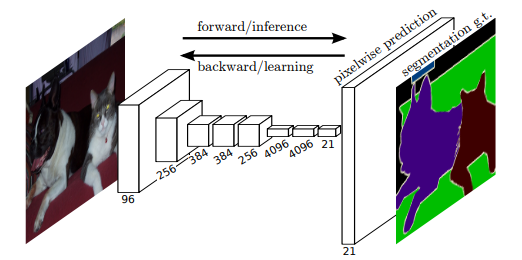
\includegraphics[width=0.9\textwidth]{figures/related_works/fcn}}
    \caption{Fully Convolutional Network (FCN) for semantic segmentation (adapted from \cite{fsss_fcn}).}
    \label{fig:fcn}
\end{figure}

The first fully convolutional network (FCN) for semantic segmentation was proposed by Long et al.~\cite{fsss_fcn}, which replaced the fully connected layers in traditional CNNs with convolutional layers, as shown in ~\autoref{fig:fcn}. This allowed the network to produce dense predictions for each pixel in the input image. The FCN architecture was further improved by adding skip connections, which helped to preserve spatial information and improve segmentation accuracy.


Then came the introduction of U-Net~\cite{fsss_unet}, a popular architecture for semantic segmentation that is widely used in medical imaging and other applications. U-Net consists of an encoder-decoder structure, where the encoder captures context information, and the decoder enables precise localization. The \emph{skip connections} between the encoder and decoder blocks play a crucial role by retaining spatial information, making U-Net particularly effective for tasks with limited training data.

The field of semantic segmentation has continued to evolve with the introduction of various architectures and techniques.

The DeepLab series~\cite{fsss_deeplabv1, fsss_deeplabv2, fsss_deeplabv3,fsss_deeplabv3plus} introduced atrous convolution and spatial pyramid pooling to capture multiscale context information; DeepLabv1~\cite{fsss_deeplabv1} also used a method called CRF (Conditional Random Field) to refine the segmentation results. But it was removed in later versions of the model. In DeepLabv2~\cite{fsss_deeplabv2}, the atrous convolution method evolved into a more general form called atrous spatial pyramid pooling (ASPP), which allows the model to capture features at multiple scales. The ASPP module consists of parallel atrous convolutions with different rates, enabling the model to learn multiscale context information effectively.

\begin{figure}[htbp]
    \centering
    \fbox{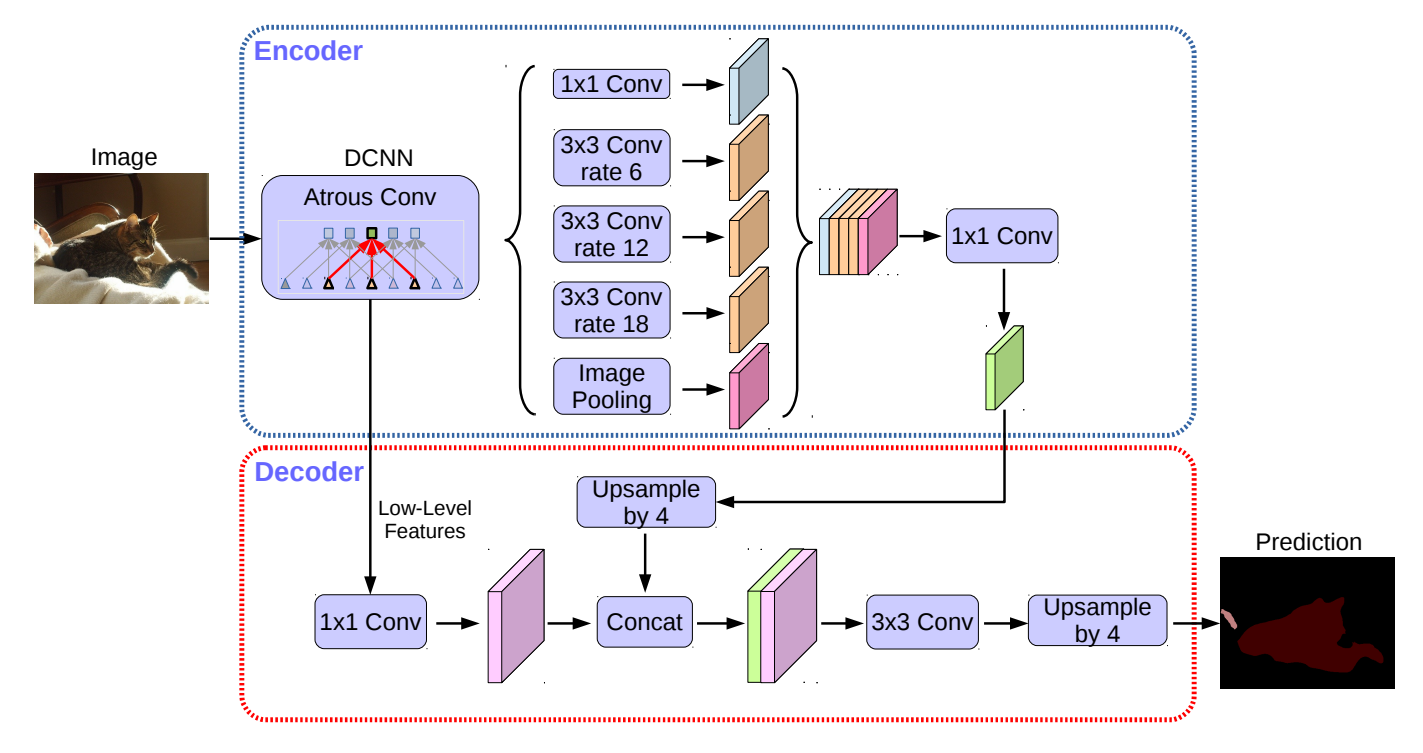
\includegraphics[width=0.9\textwidth]{figures/related_works/deeplabv3+}}
    \caption{Architecture of DeepLabv3+ (adapted from \cite{fsss_deeplabv3plus}).}
    \label{fig:dlv3+}
\end{figure}

Finally, DeepLabv3+~\cite{fsss_deeplabv3plus} introduced a new decoder module that refines the segmentation results by combining low-level features from the encoder with high-level features from the ASPP module, as shown in ~\autoref{fig:dlv3+}. This approach improves the localization of object boundaries and enhances the overall segmentation performance.

Zhao et al.~\cite{fsss_pspnet} introduced the Pyramid Scene Parsing Network (PSPNet), which uses a pyramid pooling module to capture global context information at different scales. The pyramid pooling module aggregates features from different regions of the image, allowing the model to learn rich contextual information for better segmentation.

SegNet~\cite{fsss_segnet} is an encoder-decoder architecture that focuses on efficient upsampling of feature maps.
\begin{figure}[htbp]
    \centering
    \fbox{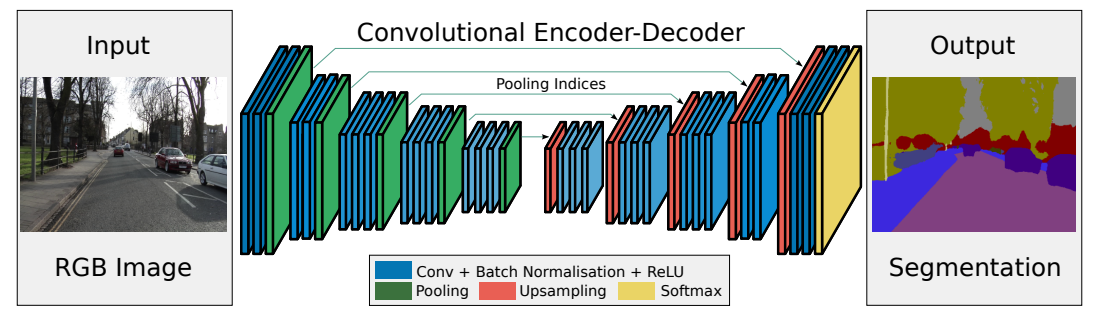
\includegraphics[width=0.9\textwidth]{figures/related_works/segnet}}
    \caption{An illustration of the SegNet architecture (adapted from \cite{fsss_segnet}).}
    \label{fig:segnet}
\end{figure}

SegNet uses a series of convolutional and pooling layers in the encoder to extract features, followed by a corresponding decoder that upsamples the feature maps to produce the final segmentation output, as demonstrated in ~\autoref{fig:segnet}. The main innovation in SegNet is the use of unpooling layers, which store the indices of the max-pooling operation during encoding, instead of the feature maps themselves. This allows for more efficient memory usage and faster inference times, making SegNet suitable for real-time applications.

\subsection{Transformers}
\label{subsec:transformers}
The introduction of transformers in computer vision has led to significant advancements in semantic segmentation. Vision Transformer (ViT) ~\cite{transformer_vit} and its variants have shown promising results in various tasks, including semantic segmentation. ViTs use self-attention mechanisms to capture long-range dependencies and global context information, making them suitable for dense prediction tasks. Later on, transformer-based architectures have gained popularity in semantic segmentation. 

Swin Transformer~\cite{transformer_swin} introduces a hierarchical architecture with shifted windows to capture both local and global context information. Swin works like a transformer but its hierarchical feature extraction is analogous to that of CNNs. It has shown state-of-the-art performance on various benchmark datasets, including ImageNet-1k~\cite{dataset_imagenet} for image classification, COCO~\cite{dataset_coco} for object detection, and ADE20K~\cite{dataset_ade20k} for semantic segmentation. The Swin Transformer has thus been widely adopted in various applications.

Leveraging the strengths of Vision Transformer, Zheng et al.~\cite{fsss_setr} first proposed the SETR (Semantic Segmentation Transformer) architecture, which replaces the traditional CNN backbone with a transformer encoder. The SETR architecture consists of a ViT encoder that processes the input image and generates a set of feature maps, followed by a decoder that upsamples the feature maps to produce the final segmentation output. The SETR model has shown competitive performance on various benchmark datasets, demonstrating the effectiveness of transformers in semantic segmentation tasks.

The Segmenter~\cite{fsss_segmenter} architecture combines a ViT backbone with a lightweight decoder for efficient semantic segmentation. 
\begin{figure}[htbp]
    \centering
    \fbox{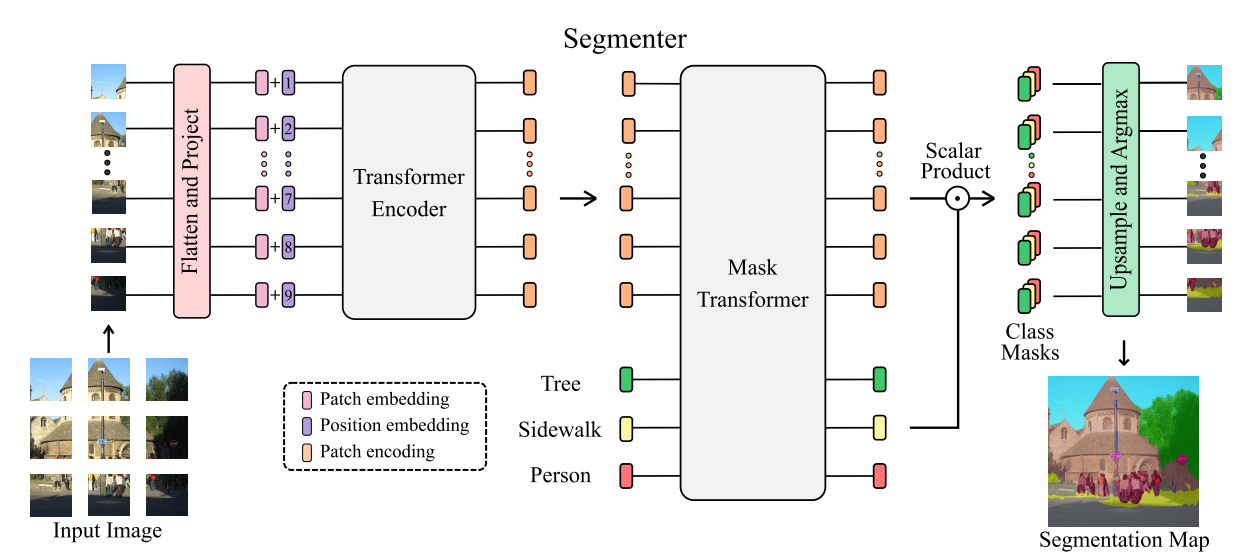
\includegraphics[width=0.9\textwidth]{figures/related_works/segmenter}}
    \caption{The Segmenter framework (adapted from \cite{fsss_segmenter}).}
    \label{fig:segmenter}
\end{figure}

The Segmenter model, as shown in ~\autoref{fig:segmenter} uses a transformer encoder to capture global context information and a simple decoder to produce the final segmentation output. The Segmenter architecture is designed to be computationally efficient while maintaining high accuracy, making it suitable for real-time applications.

SegFormer~\cite{fsss_segformer} is a transformer-based architecture that combines the strengths of both CNNs and transformers for semantic segmentation. 
\begin{figure}[htbp]
    \centering
    \fbox{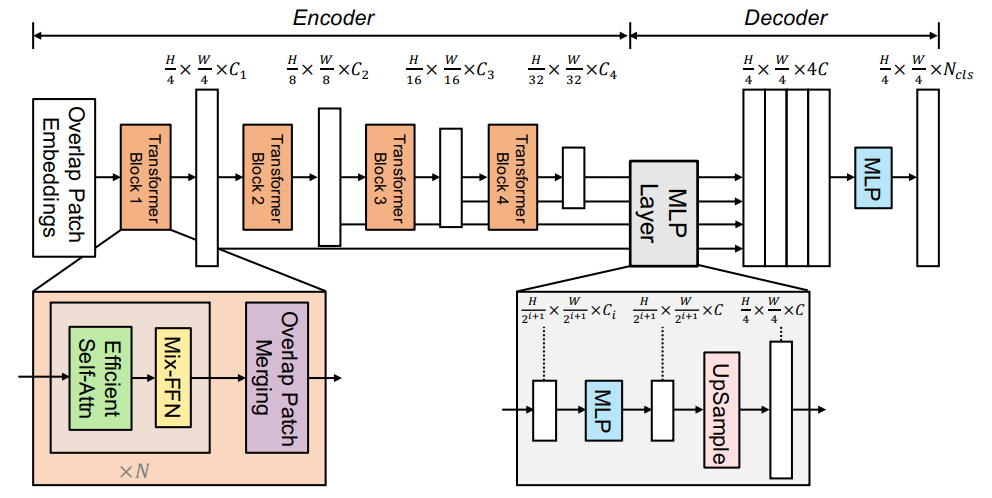
\includegraphics[width=0.9\textwidth]{figures/related_works/segformer}}
    \caption{An illustration of the SegNet architecture (adapted from \cite{fsss_segformer}).}
    \label{fig:segformer}
\end{figure}
SegFormer, as illustrated in ~\autoref{fig:segformer} uses a hierarchical transformer encoder to capture multi-scale features and a lightweight decoder to produce the final segmentation output. The SegFormer model has shown state-of-the-art performance on various benchmark datasets, demonstrating the effectiveness of combining CNNs and transformers in semantic segmentation tasks.

The field of semantic segmentation has seen significant advancements with the introduction of various architectures and techniques. The combination of CNNs and transformers has led to improved performance and efficiency in semantic segmentation tasks. As the field continues to evolve, we can expect further innovations and breakthroughs in this area.

\subsection{Problem with Fully Supervised Semantic Segmentation}
\label{subsec:problem-with-fully-supervised}
Fully supervised semantic segmentation has achieved remarkable success, largely driven by powerful models and richly annotated datasets. However, this success comes at a significant cost: acquiring dense pixel-level annotations is both expensive and time-consuming. Each image must be meticulously labeled, often requiring expert knowledge and hours of manual effort. This high annotation burden severely limits the scalability of fully supervised methods, especially for large or specialized datasets. To overcome this bottleneck, the research community has increasingly turned toward weakly supervised semantic segmentation (WSSS), an approach that seeks to train effective segmentation models with minimal supervision.

\section{Weakly Supervised Semantic Segmentation}
\label{sec:weakly-supervised}
Fully supervised semantic segmentation depends on pixel-level segmentation masks annotated by humans. However, generating such dense annotations is tedious, time consuming, and costly. Furthermore, crowd-sourced annotators must undergo special training to handle the complexity of pixel-level labeling, restricting the scale and diversity of available datasets. Consequently, most curated datasets are limited to a small set of object categories. In contrast, unlabeled or weakly annotated images can be collected in abundance, at much lower cost, and in shorter time. This has motivated research into weakly supervised semantic segmentation (WSSS) to make semantic segmentation models more scalable.


\subsection{Types of WSSS}
\label{subsec:types-weakly-supervised}
A wide range of weak supervision has been explored, including bounding boxes, scribbles, points, image-level labels,  eye tracks, free-form squiggles, or noisy web tags. Bounding boxes provide rough object boundaries, offering useful localization cues, though they still require annotators to draw accurate boxes.  Scribble-based supervision allows annotators to roughly mark object regions without outlining exact object boundaries. Point supervision, by contrast, typically uses a single annotated pixel per object, giving coarse location information. While less costly than pixel-accurate masks, these methods still involve some level of manual annotation, making large-scale labeling expensive.


\subsection{Image-Level Label Based Weak Supervision}
\label{subsec:image-level-label}
Image-level annotation represents a cost-effective and efficient form of supervision for weakly supervised semantic segmentation. Here, each training image is provided only with class labels indicating which object categories are present, but without any information about their spatial locations. The main challenge, therefore, is to correctly associate these image-level labels with the appropriate pixels in the image.

The initial approaches attempted to train segmentation models directly from image-level labels~\cite{dcnn}, but the performance was unsatisfactory. Later methods introduced discriminative localization techniques such as Class Activation Maps (CAMs)~\cite{cam}, which highlight class-relevant regions. These coarse cues were then refined using auxiliary information such as superpixels~\cite{imagelevelpixel}, segmentation proposals~\cite{imagelevelpixel}, or motion information from videos~\cite{wsss_motion_cues}. Some works, such as Adversarial Erasing~\cite{adversarial_erasing}, expanded object coverage progressively by iteratively searching new regions. Others, like Kolesnikov and Lampert \cite{kolesnikov2016}, trained networks to approximate the dense CRF \cite{krähenbühl} applied on CAMs for refinement.

Some approaches learn to predict affinity matrices at the pixel level [36], to refine the output of dCRF through random walk. AffinityNet \cite{wsss_affinitynet} predicts class-agnostic pixel affinities to propagate CAM activations via random walks. Similarly, Seeded Region Growing (SRG) \cite{srg} expands initial seed regions using similarity criteria, while its deep learning extension DSRG \cite{wsss_dsrg_deep_seeded_region_growing} leverages high-level semantic features to grow regions more effectively. P2P \cite{pixel_to_prototype} further narrows the supervision gap by using pixel-to-prototype contrastive learning. However, a common limitation is that most of these CNN-based methods inherit the restricted locality of convolutional features.

Recent advances incorporate transformers into WSSS \cite{camtokens, getam}. TS-CAM \cite{camtokens} leverages the global information capturing ability of ViT by combining class-token attention with CAMs. \cite{getam} refines class-specific maps by using attention gradients. MCTformer \cite{wsss_MCTformer} expands this idea by embedding multiple class tokens to learn attention maps for different categories. AFA \cite{wsss_afa_affinity_from_attention} instead derives semantic affinities directly from attention maps to refine coarse pseudo-labels. WeCLIP \cite{wsss_frozen_clip} pushes this further by exploiting the frozen CLIP backbone to generate high-quality pseudo-labels, which are dynamically updated using a refinement module (RFM).

\subsection{Class Activation Maps}
\label{subsec:class-activation-maps}

Class Activation Maps (CAMs) serve as a crucial interpretability mechanism in deep learning, enabling the visualization of spatial regions within an image that most strongly influence a model's classification decisions. By highlighting class-discriminative areas, CAMs facilitate a deeper understanding of the model's internal reasoning and are foundational for generating localization cues in weakly supervised semantic segmentation. This section provides a comprehensive overview of CAM generation methodologies, with particular emphasis on their implementation in advanced frameworks such as UniCL and architectures like the Swin Transformer.

\subsubsection{Basic Classification}
\label{subsec:basic_classification}

In a standard image classification task, the model learns to assign input images to specific categories. To generate CAMs, global average pooling is applied to the feature maps from the final convolutional layer, condensing spatial information into a single vector. This process produces a heatmap that emphasizes the image regions most influential for the model's classification decision.

\begin{figure}[htbp]
    \centering
    \fbox{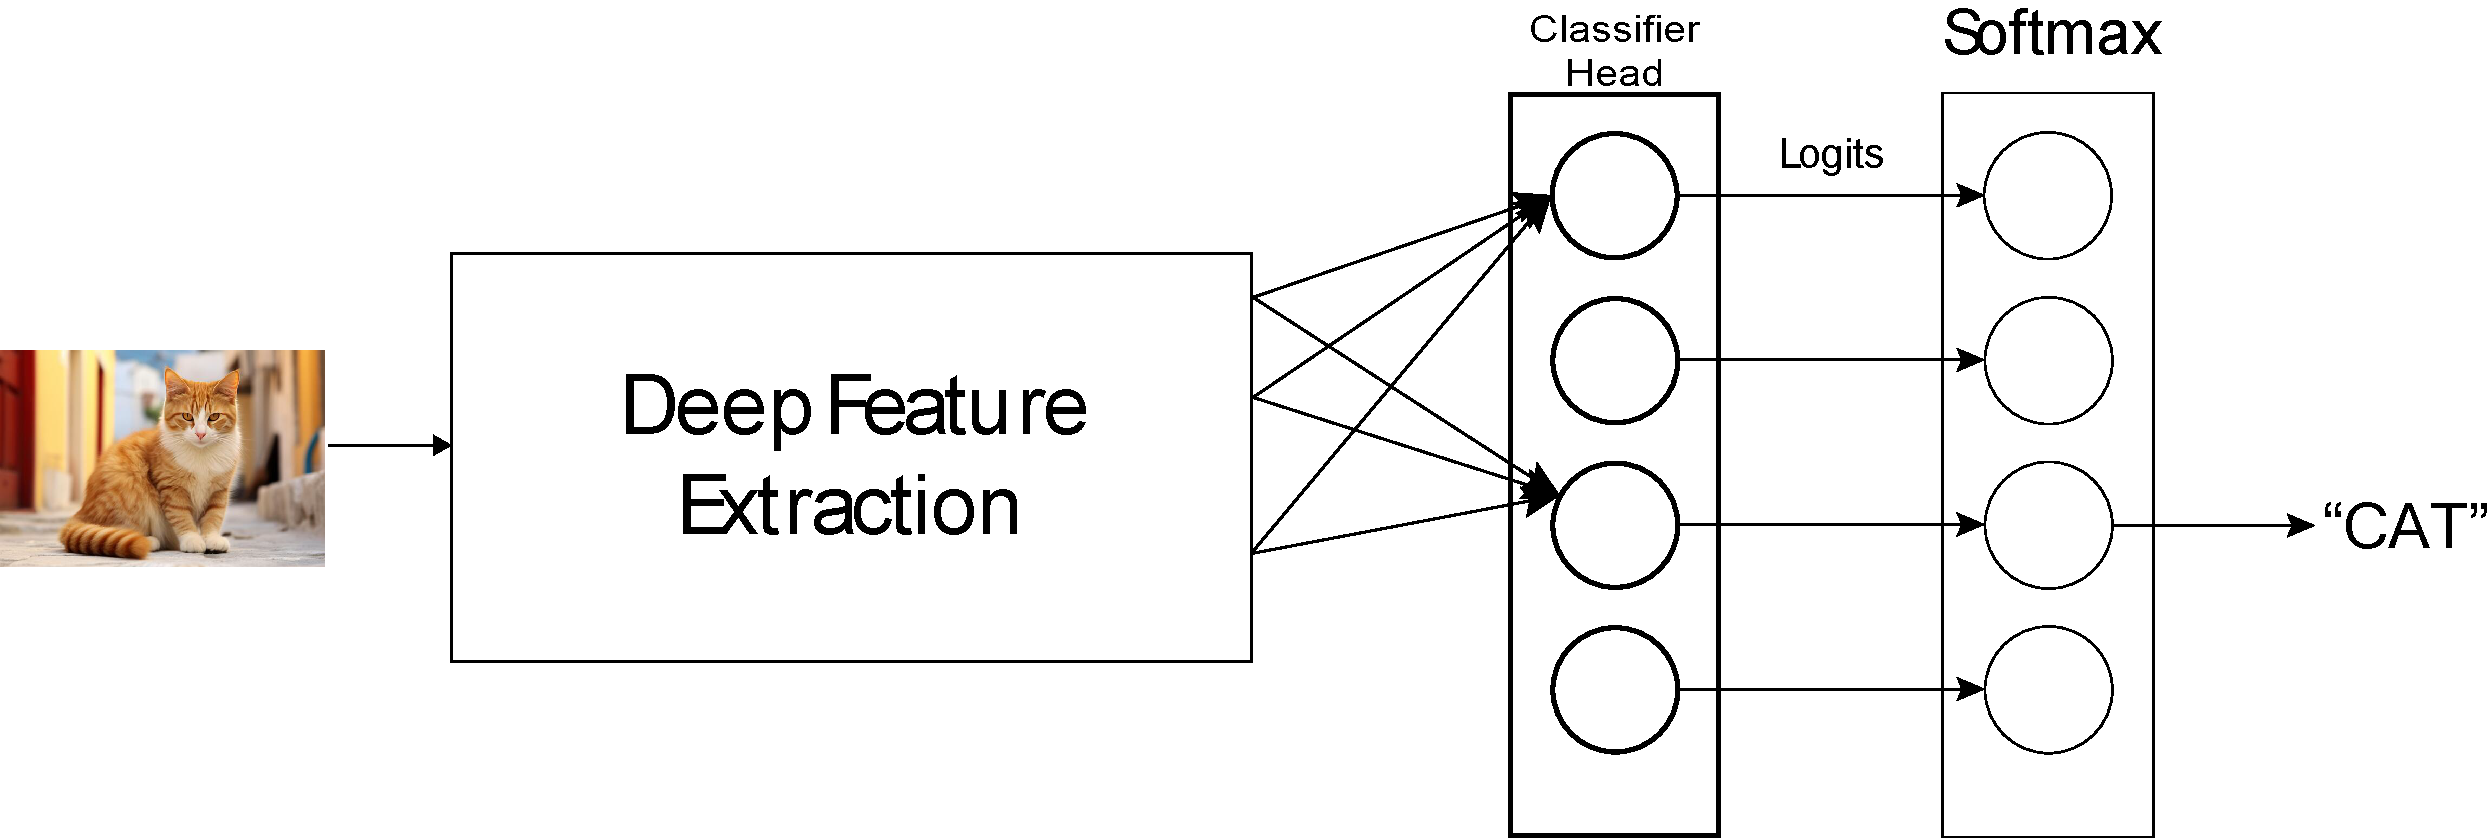
\includegraphics[width=0.8\textwidth]{basic-classification}}
    \caption{Basic Classification}
    \label{fig:basic_classification}
\end{figure}


In the ~\autoref{fig:basic_classification}, we can see a high-level overview of the basic classification task. The process can be summarized as follows:

\begin{enumerate}
    \item The input image is passed through the model, and the feature maps are generated. This deep feature extraction block can be either CNNs (as it initially was) or Transformers.
    \item The \emph{MLP (Multi-Layer Perceptron)}, also called the \emph{Classifier head}, is used to produce the final classification scores.
    \item The scores are then normalized using a \emph{softmax} function to obtain the class probabilities.
\end{enumerate}

No matter how the feature maps are generated or what the backbone is, the MLP head is used to produce the final classification scores. For CAM generation, we only need the feature maps and the class scores, i.e, upto the Classifier head.

Convolutional Neural Networks (CNNs) are often considered “black-box” models due to the limited interpretability of their internal decision-making process. To address this, Class Activation Mapping (CAM) was introduced by Zhou et al.~\cite{cam}, demonstrating that CNNs can act as unsupervised object detectors by highlighting discriminative image regions relevant to classification. CAM and its variants have since become central to Weakly Supervised Semantic Segmentation (WSSS), where such localization cues are refined into pixel-level pseudo-labels for segmentation training.

\subsubsection{Vanilla CAM}

The original CAM~\cite{cam} requires a specific network architecture where fully connected layers are replaced by a Global Average Pooling (GAP) layer followed by a linear classifier. The process is illustrated in \autoref{fig:basic_cam_generation_process}:

\begin{figure}[htbp]
    \centering
    \fbox{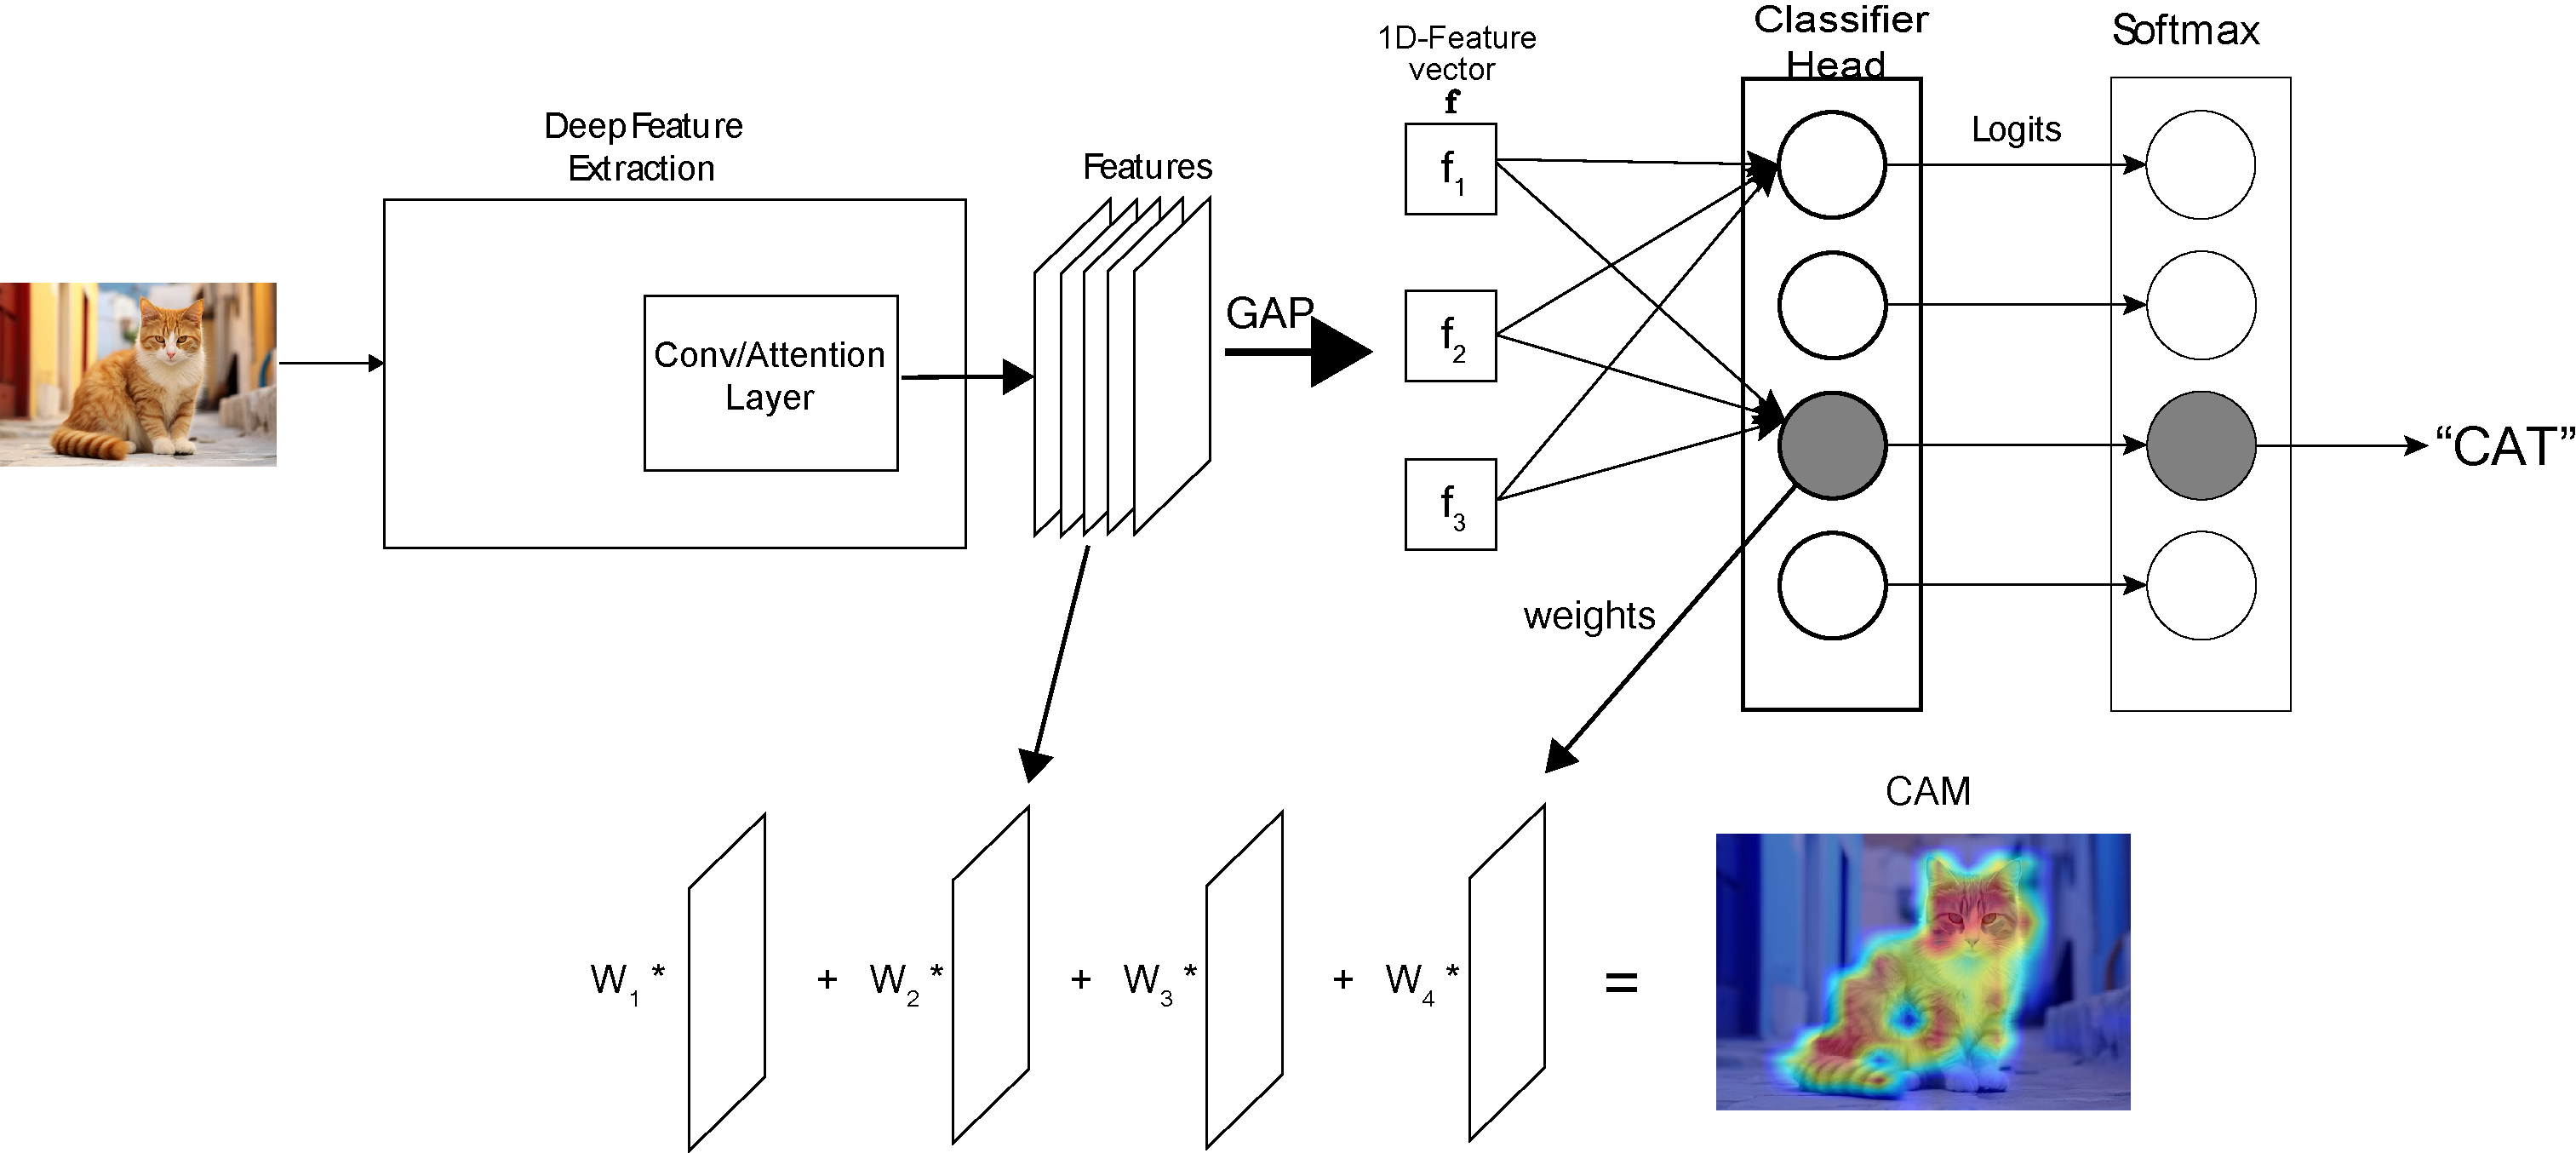
\includegraphics[width=0.95\textwidth]{basic-CAM}}
    \caption{CAM Generation Process}
    \label{fig:basic_cam_generation_process}
\end{figure}

\begin{enumerate}
    \item The input image is passed through a CNN to obtain convolutional feature maps.
    \item GAP is applied to produce a compact vector representation of the image.
    \item This representation is fed into the classifier head to generate class scores.
    \item The neuron corresponding to the predicted class is identified.
    \item The learned weights associated with this class are used to compute a weighted sum of the feature maps, yielding a class-specific heatmap.
    \item The heatmap is upsampled to match the original image resolution for visualization.
\end{enumerate}

Although effective, CAM requires the network to be modified by inserting GAP, which limits its general applicability.

\subsubsection{Grad-CAM}
\label{subsec:grad_cam}

To overcome CAM's architectural constraint, Selvaraju et al.~\cite{cam_grad} proposed Gradient-weighted CAM (Grad-CAM). Unlike CAM, Grad-CAM can be applied to any CNN-based model without requiring structural changes. Instead of relying solely on classifier weights, Grad-CAM leverages the gradient of the target class score with respect to feature maps. The process is illustrated in \autoref{fig:grad_cam_generation_process}:

\begin{figure}[htbp]
    \centering
    \fbox{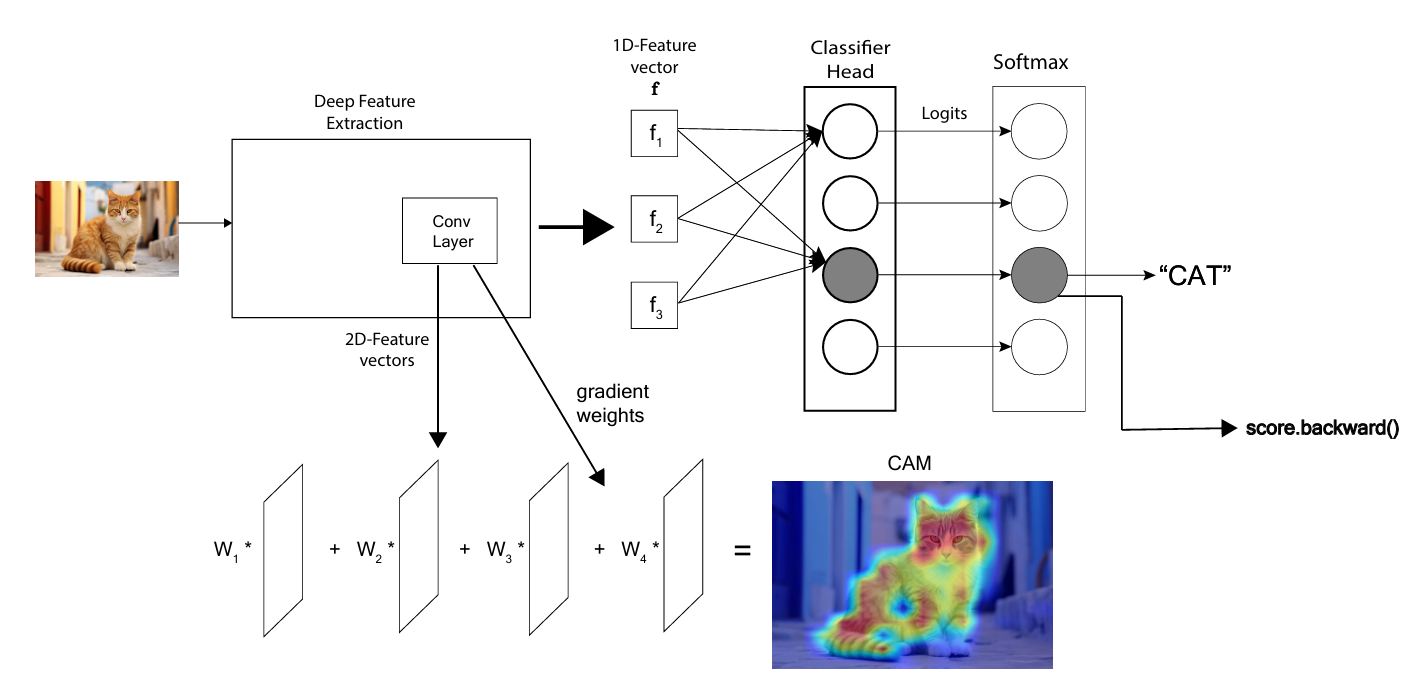
\includegraphics[width=0.98\textwidth]{figures/GRAD-CAM.png}}
    \caption{Grad-CAM Generation Process}
    \label{fig:grad_cam_generation_process}
\end{figure}

\begin{enumerate}
    \item Forward pass the input to obtain feature maps from the last convolutional layer.
    \item Compute the classification scores through the classifier head.
    \item Select the target class neuron (often the top prediction, but any class can be chosen).
    \item Backpropagate to compute gradients of this class score with respect to the feature maps.
    \item Average the gradients spatially to obtain weights for each feature map channel.
    \item Combine the feature maps using these weights to create a coarse localization heatmap.
    \item Apply ReLU to suppress negative contributions.
    \item Upsample the heatmap to align with the input image.
\end{enumerate}

Grad-CAM preserves the architectural flexibility missing in CAM, while still providing class-discriminative localization.

\subsubsection{Grad-CAM++}
Grad-CAM++~\cite{cam_gradpp} was proposed to address two main limitations of Grad-CAM: (1) poor handling of multiple object instances of the same class, and (2) sensitivity to object size and distribution. Instead of relying only on first-order gradients, Grad-CAM++ incorporates higher-order derivatives of the class score with respect to feature maps.

\begin{enumerate}
    \item The forward pass generates feature maps as in Grad-CAM.
    \item For the target class, first-order and higher-order gradients are computed.
    \item These gradients are used to calculate the pixel-wise weights, where each spatial location contributes differently to the final importance score.
    \item The weighted sum of the feature maps is constructed using these refined weights, resulting in a sharper and more spatially precise heatmap.
    \item Like Grad-CAM, the heatmap is processed with ReLU and upsampled.
\end{enumerate}

This method improves localization in complex scenarios, such as small objects or multiple instances, while requiring only one backward pass, keeping computational costs similar to Grad-CAM.

\subsubsection{LayerCAM}
LayerCAM\cite{layer_cam} builds on the intuition that meaningful localization is not limited to the last convolutional layer. Earlier and intermediate layers often capture fine-grained features such as edges and textures, which can complement coarse semantic features from deeper layers.

LayerCAM\cite{layer_cam} computes CAMs at multiple levels of the network:
\begin{enumerate}
    \item For each chosen convolutional layer, the gradients with respect to the target class are calculated.
    \item Instead of spatially averaging the gradients, LayerCAM\cite{layer_cam} assigns weights at every spatial location by multiplying activation values with their corresponding gradients.
    \item These location-aware weights allow the method to produce more precise heatmaps per layer.
    \item CAMs from different layers are then combined to form a multiscale localization map that captures both coarse object regions and fine details.
\end{enumerate}

By integrating multilayer signals, LayerCAM\cite{layer_cam} enhances both interpretability and localization accuracy compared to Grad-CAM.

\subsubsection{Attention Rollout and Attention Flow}
Beyond CNN-based visualization, transformer-based networks introduced attention-based interpretability. Abnar and Zuidema~\cite{attention_rollout} proposed two techniques:

- \textbf{Attention Rollout}: Recursively multiplies the attention matrices across layers, incorporating residual connections. This assumes that the token identity propagates linearly through attention weights, providing a global view of how input tokens influence the final decision. \\
- \textbf{Attention Flow}: Formulates interpretability as a maximum flow problem, modeling information propagation as a flow network. A maximum flow algorithm is then applied to trace how embeddings in deeper layers are connected back to input tokens.

Both methods generate token-level importance maps that correlate strongly with gradient-based measures, improving interpretability for transformer architectures.

\subsubsection{RelevanceCAM}
RelevanceCAM~\cite{relevance_cam} incorporates Layer-wise Relevance Propagation (LRP) into CAM generation. Unlike gradient-based methods that can suffer from the shattered gradient problem, LRP redistributes the prediction score backward through the network based on relevance conservation principles.

\begin{enumerate}
    \item Starting from the target class score, relevance values are propagated layer by layer toward the input.
    \item Each neuron's contribution is quantified based on how much it supports the class prediction.
    \item These relevance scores are aggregated spatially to form heatmaps in multiple layers.
    \item The final activation map combines information from both shallow and deep layers, enhancing robustness and interpretability.
\end{enumerate}

RelevanceCAM~\cite{relevance_cam} provides more stable and faithful explanations, particularly in intermediate layers, and demonstrates improved localization performance over traditional Grad-CAM variants.

\subsubsection{Summary}
Overall, CAM-based methods have evolved from the original GAP-based CAM~\cite{cam} to gradient-driven approaches like Grad-CAM~\cite{cam_grad}, higher-order generalizations such as Grad-CAM++~\cite{cam_gradpp}, multi-layer extensions like LayerCAM~\cite{layer_cam}, attention-based methods for transformers~\cite{attention_rollout}, and LRP-driven methods like RelevanceCAM~\cite{relevance_cam}. These advances have been pivotal in WSSS, where class-discriminative heatmaps serve as initial localization cues that are refined into pixel-level pseudo-labels for segmentation.

\section{Component-Wise Literature Review of WSSS Models}
\label{sec:how-wsss-models-work}

\subsection{Feature Extraction From Backbone}
\label{subsec:feature-extraction-backbone}

The architecture of AffinityNet \cite{wsss_affinitynet} relies on three DNNs: a classification network for generating CAMs, the AffinityNet module itself, and a segmentation network. 
\begin{figure}[htbp]
    \centering
    \fbox{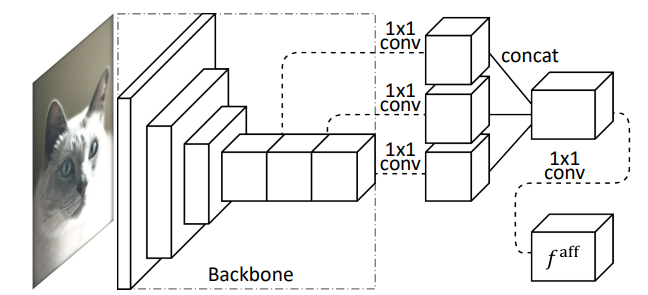
\includegraphics[width=0.8\textwidth]{figures/related_works/affinitynet}}
    \caption{Overall architecture of AffinityNet (adapted from \cite{wsss_affinitynet}).}
    \label{fig:affinitynet}
\end{figure}

All three share the same backbone, as illustrated in ~\autoref{fig:affinitynet}. The backbone is a modified variant of Model A1 \cite{RevisitingResNET}, commonly referred to as ResNet38, which consists of 38 convolutional layers with wider channels. In this adaptation, the GAP and fully connected layers from the original design are removed, and the final three convolutional stages are replaced with atrous convolutions with stride 1. The dilation rates are adjusted so that the resulting feature maps maintain a stride of 8.

In DSRG \cite{wsss_dsrg_deep_seeded_region_growing}, the classification branch employs a slightly altered version of the 16-layer VGG model \cite{VGG16}, while the segmentation branch is built upon DeepLabv2 \cite{fsss_deeplabv2}. Both are initialized with VGG-16 weights pre-trained on ImageNet.

AFA \cite{wsss_afa_affinity_from_attention} adopts the Mix Transformer (MiT) backbone introduced in SegFormer \cite{fsss_segformer}, which is more suitable for image segmentation tasks compared to the vanilla ViT. The MiT parameters are initialized using ImageNet-1k pre-trained weights.

ToCo \cite{wsss_toco_token_contrast} uses the ViT-Base (ViT-B) backbone initialized with ImageNet pre-trained weights. Within the ViT encoder, an auxiliary classification head is introduced to produce CAMs. These auxiliary CAMs are then used to form pseudo labels guiding the Pixel-Token Contrast (PTC) module, and also to generate proposals for cropping positive and negative local patches for the Cross-Token Contrast (CTC) module. The final CAM is generated through the classification layer and subsequently transformed into pseudo labels.

CLIP-ES \cite{wsss_clip_es} employs the CLIP ViT-B/16 backbone, where the image encoder extracts visual features and the text encoder extracts linguistic features. Since CLIP is pre-trained on roughly 400 million image-text pairs, it provides strong multimodal representations for segmentation.

\begin{figure}[htbp]
    \centering
    \fbox{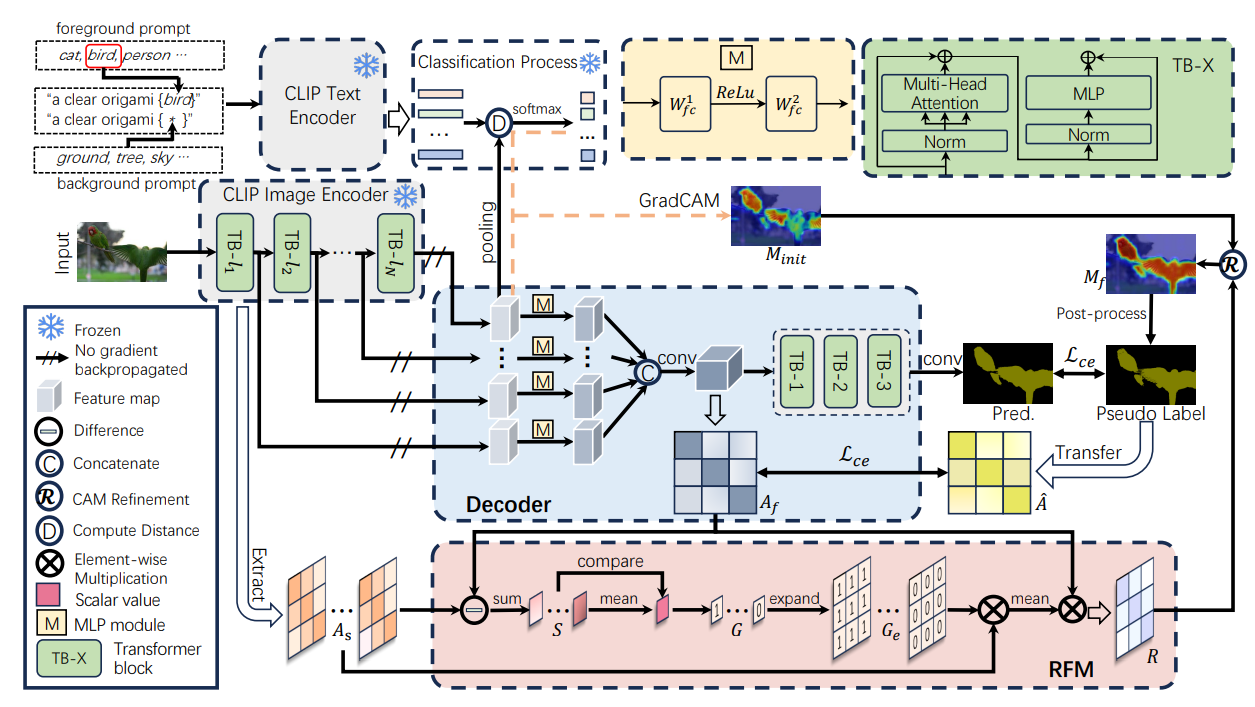
\includegraphics[width=0.9\textwidth]{figures/related_works/frozenclip}}
    \caption{Overall architecture of WeCLIP (adapted from \cite{wsss_frozen_clip}).}
    \label{fig:frozenclip}
\end{figure}

The whole framework of WeCLIP\cite{wsss_frozen_clip} consists of four major components: a frozen CLIP backbone (comprising a ViT-Base/16 image encoder and a text encoder) \cite{transformer_vit}, a classification module for generating initial CAMs, a decoder for segmentation prediction, and a refinement module (RFM) to enhance CAMs into pseudo labels for supervision, as shown in ~\autoref{fig:frozenclip}.

\subsection{CAM Generation}
\label{subsec:cam-generation}
In AffinityNet \cite{wsss_affinitynet}, CAMs are generated by appending three layers to the backbone: a 3×3 convolutional layer with 512 channels for task adaptation, a global average pooling layer to aggregate spatial information, and a fully connected layer for classification. The class activation maps are computed by weighting the feature maps with the class-specific weights from the final layer. These maps are normalized such that their maximum value is 1, and the background map is obtained by subtracting the maximum class activation at each pixel from 1.

In DSRG \cite{wsss_dsrg_deep_seeded_region_growing}, CAMs \cite{cam} are used to localize foreground regions. The classification branch applies a fully connected layer to the conv7 features, producing a heatmap for each class. Foreground seed cues are extracted by thresholding these heatmaps, while background cues are identified from regions in normalized saliency maps with low pixel intensities.

AFA \cite{wsss_afa_affinity_from_attention} similarly employs CAMs to generate initial pseudo labels. These maps are formed by linearly combining feature maps from the classification layer using learned weights, followed by a ReLU activation to suppress negative values. The outputs are then scaled to the [0,1] range, and an additional background score is included to differentiate foreground from the background.

ToCo \cite{wsss_toco_token_contrast} incorporates an auxiliary classification layer to extract semantic information and produce CAMs. Patch tokens are aggregated using global max pooling and subsequently passed through a fully connected layer, resulting in auxiliary CAMs that guide the model's training.

In WeCLIP\cite{wsss_frozen_clip}, image features are extracted from the frozen CLIP image encoder, while class-specific text prompts are processed by the CLIP text encoder, both remaining fixed during training. Classification scores are calculated as distances between pooled image and text features, and Grad-CAM \cite{cam_grad} is applied to these scores to generate the initial CAMs.


\subsection{Pseudo Label Generation}
\label{subsec:pseudo-label-generation}
AffinityNet\cite{wsss_affinitynet} predicts convolutional feature maps in which the semantic affinity between two feature vectors is measured using their L1 distance. To train this network, semantic affinity labels are derived from CAMs. Specifically, confident foreground and background regions are identified, while ambiguous regions are treated as neutral. Pairwise affinities are then defined according to class labels — assigned as 1 for pixels of the same class, 0 for different classes, and ignored for neutral labels. Once trained, AffinityNet refines CAMs through a random walk guided by the semantic transition matrix, thereby enhancing CAM quality and producing more accurate pseudo segmentation labels.

In DSRG\cite{wsss_dsrg_deep_seeded_region_growing}, pseudo labels are generated by expanding initial seed cues into unlabeled regions using the classical Seeded Region Growing (SRG) algorithm \cite{srg}. For each class, the seed cues are visited in row first manner and its 8-connectivity neighborhood pixels are checked for similarity criteria. If they satisfy the criteria , those pixels are added to the set of seed cues for that particular class, and this process is repeated for every object class. The dynamically updated seed sets act as supervision, continuously refining pseudo labels during training.

\begin{figure}[htbp]
    \centering
    \fbox{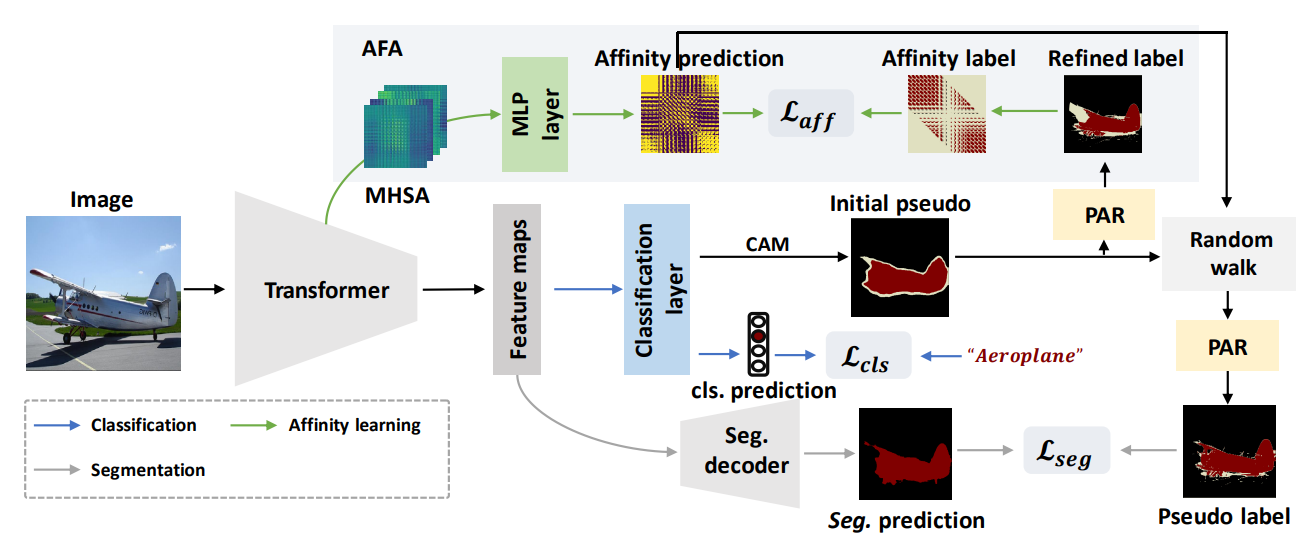
\includegraphics[width=0.9\textwidth]{figures/related_works/afa}}
    \caption{AFA framework for WSSS (adapted from \cite{wsss_afa_affinity_from_attention}).}
    \label{fig:afa}
\end{figure}

The AFA\cite{wsss_afa_affinity_from_attention} module computes semantic affinities directly by linearly combining multi-head attention outputs through an MLP layer. To ensure matrix symmetry, the affinity matrix is summed with its transpose, under the assumption that nodes with the same semantics should be equivalent. 

Supervision is provided by pseudo affinity labels derived from refined CAMs: pixels are assigned to the class with the highest activation, and affinities are set positive if two pixels share the same class; otherwise negative. These pseudo affinity labels supervise the affinity prediction process, as shown in ~\autoref{fig:afa}. The learned semantic affinities are then used in a random walk propagation to refine the CAMs.

In ToCo\cite{wsss_toco_token_contrast}, auxiliary CAMs are segmented into pseudo token labels by applying two background thresholds, categorizing tokens into reliable foreground, background, and uncertain regions. Positive token pairs are defined as those sharing the same label, while others are treated as negative. To counteract over-smoothing, the Patch Token Contrast (PTC) module maximizes similarity between positive pairs of patch tokens and minimizes it for negative ones. 
\begin{figure}[htbp]
    \centering
    \fbox{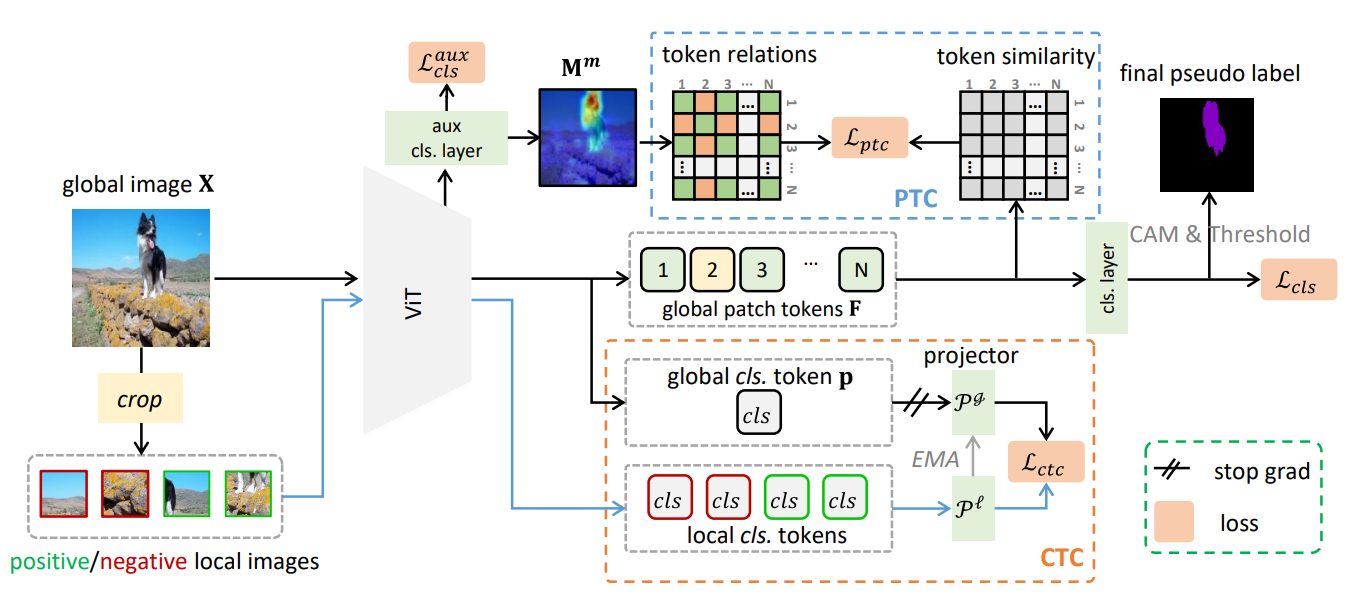
\includegraphics[width=0.9\textwidth]{figures/related_works/toco}}
    \caption{Overall framework of ToCo (adapted from \cite{wsss_toco_token_contrast}).}
    \label{fig:toco}
\end{figure}
Additionally, as shown in ~\autoref{fig:toco}, the Class Token Contrast (CTC) module enforces consistency across entire object regions by aligning representations of global and local class tokens. Specifically, it reduces the gap between projected global class tokens and projected local tokens cropped from uncertain or background regions, thereby improving pseudo label quality.

\subsection{Segmentation Prediction}
\label{subsec:segmentation-prediction}
In AffinityNet\cite{wsss_affinitynet}, the segmentation model is constructed by adding two atrous convolution layers on top of the backbone. The segmentation predictions are then supervised using refined CAMs, which are generated by propagating pairwise pixel affinities.

For DSRG\cite{wsss_dsrg_deep_seeded_region_growing}, once seed cues are obtained from initial CAMs, an image semantic segmentation network is trained with these cues. A balanced seeding loss is applied so that the network's predictions are encouraged to match only the seed regions defined by the classification network, while ignoring unlabeled pixels. As training progresses, the seed cues are iteratively refined into pseudo labels, and the segmentation model is retrained with the updated supervision.

In ToCo\cite{wsss_toco_token_contrast}, the segmentation decoder is deliberately simple, consisting of two 3×3 convolutional layers (each with dilation rate 5) followed by a 1×1 prediction layer. The pseudo labels produced by ToCo are passed through a Pixel-Adaptive Refinement (PAR) module, and the improved labels serve as supervision for the decoder to generate the final segmentation output.

For AFA\cite{wsss_afa_affinity_from_attention}, an MLP-based decoder head is employed. This head fuses features across multiple levels through lightweight MLP layers to produce segmentation predictions. The supervision is provided by refined pseudo labels obtained through affinity propagation.

In WeCLIP\cite{wsss_frozen_clip}, segmentation is guided by a feature decoder that extracts intermediate outputs from each transformer block of the CLIP image encoder. For each feature map, a dedicated MLP is applied to generate enhanced feature representations, which are concatenated and then passed through a convolutional layer to form a fused feature map. This fused representation is subsequently processed by multiple stacked multi-head transformer blocks, producing the final segmentation prediction P.

\subsection{Refinement of Pseudo Labels}
\label{subsec:refinement-of-pseudo-labels}
A major challenge in weakly supervised semantic segmentation is the generation of high-quality pseudo labels from weak annotations. The quality of these pseudo labels directly impacts the performance of the segmentation model. Therefore, refinement techniques are often employed to improve the quality of the pseudo labels. These techniques can include post-processing methods, such as conditional random fields (CRFs), or affinity based methods that leverage the relationships between pixels to refine the segmentation results.

AffinityNet \cite{wsss_affinitynet} is a notable example of a refinement technique that uses affinity information to improve the segmentation results. After generating initial CAMs from image-level labels, AffinityNet trains a CNN network to classify whether two adjacent pixels belong to the same semantic region. A random walk algorithm, using these affinities, then propagates object labels across the image, enhancing coherence of the segmentation masks.

\begin{figure}[thbp]
    \centering
    \fbox{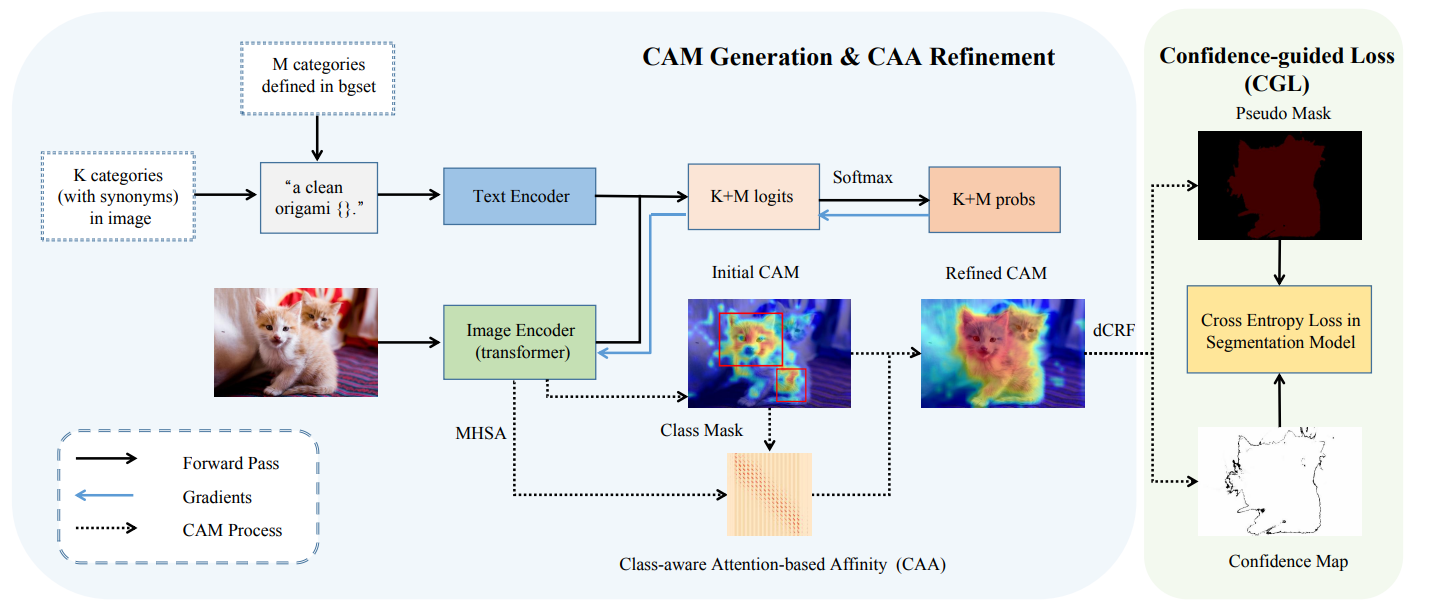
\includegraphics[width=0.9\textwidth]{figures/related_works/clipes}}
    \caption{Overview of CLIP-ES framework (adapted from \cite{wsss_clip_es}).}
    \label{fig:clipes}
\end{figure}

AFA \cite{wsss_afa_affinity_from_attention} advanced this idea by showing that pixel affinities can be efficiently derived from attention maps of vision transformers, rather than training a separate affinity prediction network. Specifically, AFA extracts affinity information from the self-attention layers of the transformer backbone, using which it performs random walk propagation like AffinityNet. This approach simplifies the refinement pipeline and benefits from the strong semantic relationships already captured by attention mechanisms. In addition, it introduces the Pixel Adaptive Refinement (PAR) module, which uses local color and spatial information to further refine the initial pseudolabels. PAR is based on pixel adaptive convolution and less costly compared to DCRFs. It also dilates the kernels to cover a larger area, allowing it to capture more contextual information.

CLIP-ES \cite{wsss_clip_es} uses a similar approach, but instead of using the attention maps from the transformer, it uses the attention maps from the CLIP model. The CLIP model is a powerful vision-language model that has been shown to be effective in object detection and segmentation tasks. 

By leveraging the attention maps from the CLIP model, CLIP-ES is able to generate high-quality pseudo labels that are more accurate and robust than those generated by traditional methods. It uses the random walk propagation like AFA, along with a bounding box mask to mask certain affinities while covering more object regions, as shown in ~\autoref{fig:clipes}.

WeCLIP\cite{wsss_frozen_clip} is another technique that uses the CLIP model to generate pseudo labels. In addition to using the attention maps from the CLIP model, it uses the decoder to generate pseudo labels. Since its backbone is frozen, it requires a decoder to enable the model to learn the affinities of the features. Then it weights the decoder affinities with the frozen CLIP attention maps to get the final affinity map. After that, it uses the random walk propagation with box mask like CLIP-ES and applies the PAR module of AFA to get the final segmentation pseudo labels.

\section{WSSS Training Approaches}
\label{sec:stages}

Weakly supervised semantic segmentation has two main solutions based on their training processes: multistage approaches \cite{instance_wsss,wsss_L2G,wsss_rib} and single stage approaches \cite{wsss_reliability_does_matter, wsss_afa_affinity_from_attention}.

\subsection{Multistage}
\label{subsec:multi-stage}

Multistage WSSS has multiple steps. Typically, a classification model is first trained to generate the CAM,  which are then converted into initial pixel-level pseudo labels. These pseudo labels are refined through affinity matrix and random walk propagation\cite{wsss_affinitynet, wsss_afa_affinity_from_attention}, or seeded region growing[SRG] or contrastive learning. Then these refined pseudo labels are used for supervising a segmentation model.

Du et al. \cite{pixel_to_prototype} introduced a pixel-to-prototype contrastive method that enforces semantic consistency at the feature level, leading to improved pseudo-label quality. MCTformer \cite{wsss_MCTformer} extended transformer-based models with multiple class tokens, enabling the generation of category-specific attention maps for refined CAMs. More recently, researchers have incorporated CLIP into the WSSS pipeline. For instance, CLIMS \cite{wsss_clims} used CLIP to highlight more complete object regions while suppressing confident background activations. Similarly, CLIP-ES \cite{wsss_clip_es} applied a softmax-based GradCAM \cite{cam_grad} guided by carefully designed text prompts, allowing CLIP to produce reliable pseudo labels for segmentation supervision.

\subsection{Single Stage}
\label{subsec:single-stage}

In single-stage weakly supervised semantic segmentation, the model tries to learn segmentation directly from weak supervision (like image-level labels) in one shot. A network is trained that produces segmentation outputs without going through separate phases of label generation and refinement. There's no explicit intermediate step to improve pseudo labels — the model directly predicts segmentation maps during training based on weak supervision signals.

Earlier work in this line used ImageNet-pretrained backbones \cite{dataset_imagenet} to jointly optimize classification and segmentation, with most efforts devoted to improving supervision quality or constraining the learning process. AA\&AR \cite{wsss_aaar} proposed an adaptive affinity loss that facilitates semantic propagation within the segmentation branch. AFA \cite{wsss_afa_affinity_from_attention} introduced an affinity branch to refine CAMs online, yielding stronger pseudo labels during training. ToCo \cite{wsss_toco_token_contrast} further advanced this direction by employing token-level contrastive learning to mitigate over-smoothing in CAM generation, thereby providing better online supervision.

% \section{Summary}
% \label{sec:summary-related-works}

In summary, weakly supervised semantic segmentation has evolved significantly, with various types of weak supervision being explored. Image-level labels have emerged as a cost-effective form of supervision, leading to the development of techniques like Class Activation Maps (CAMs) for localization. Numerous methods have been proposed to refine these CAMs into high-quality pseudo labels, leveraging affinity matrices, random walk propagation, and contrastive learning. Both multistage and single-stage training approaches have been employed, each with its own advantages. Recent advancements have also integrated powerful models like CLIP to enhance pseudo label generation. Overall, these developments have contributed to more effective and scalable WSSS models.
\chapter{Proposed Methodology}
\label{chap:methodology}

In our proposed methodology, we aim to leverage the strengths of both the UniCL framework and the Swin Transformer architecture to enhance the performance of our model. The methodology is structured into several key components, each addressing a specific aspect of the overall process. The following sections provide a detailed overview of each component, including the backbone architecture, CAM generation, pseudo label generation, segmentation prediction, and refinement.

\section{Overview}
\label{sec:overview}
In this section, we provide a high-level overview of the proposed methodology. The methodology is designed to address the challenges of weakly supervised semantic segmentation (WSSS) by leveraging the strengths of multi-modal learning frameworks like UniCL and advanced vision architectures such as the Swin Transformer. The key components of the methodology include:

\begin{figure}
    \centering
    \fbox{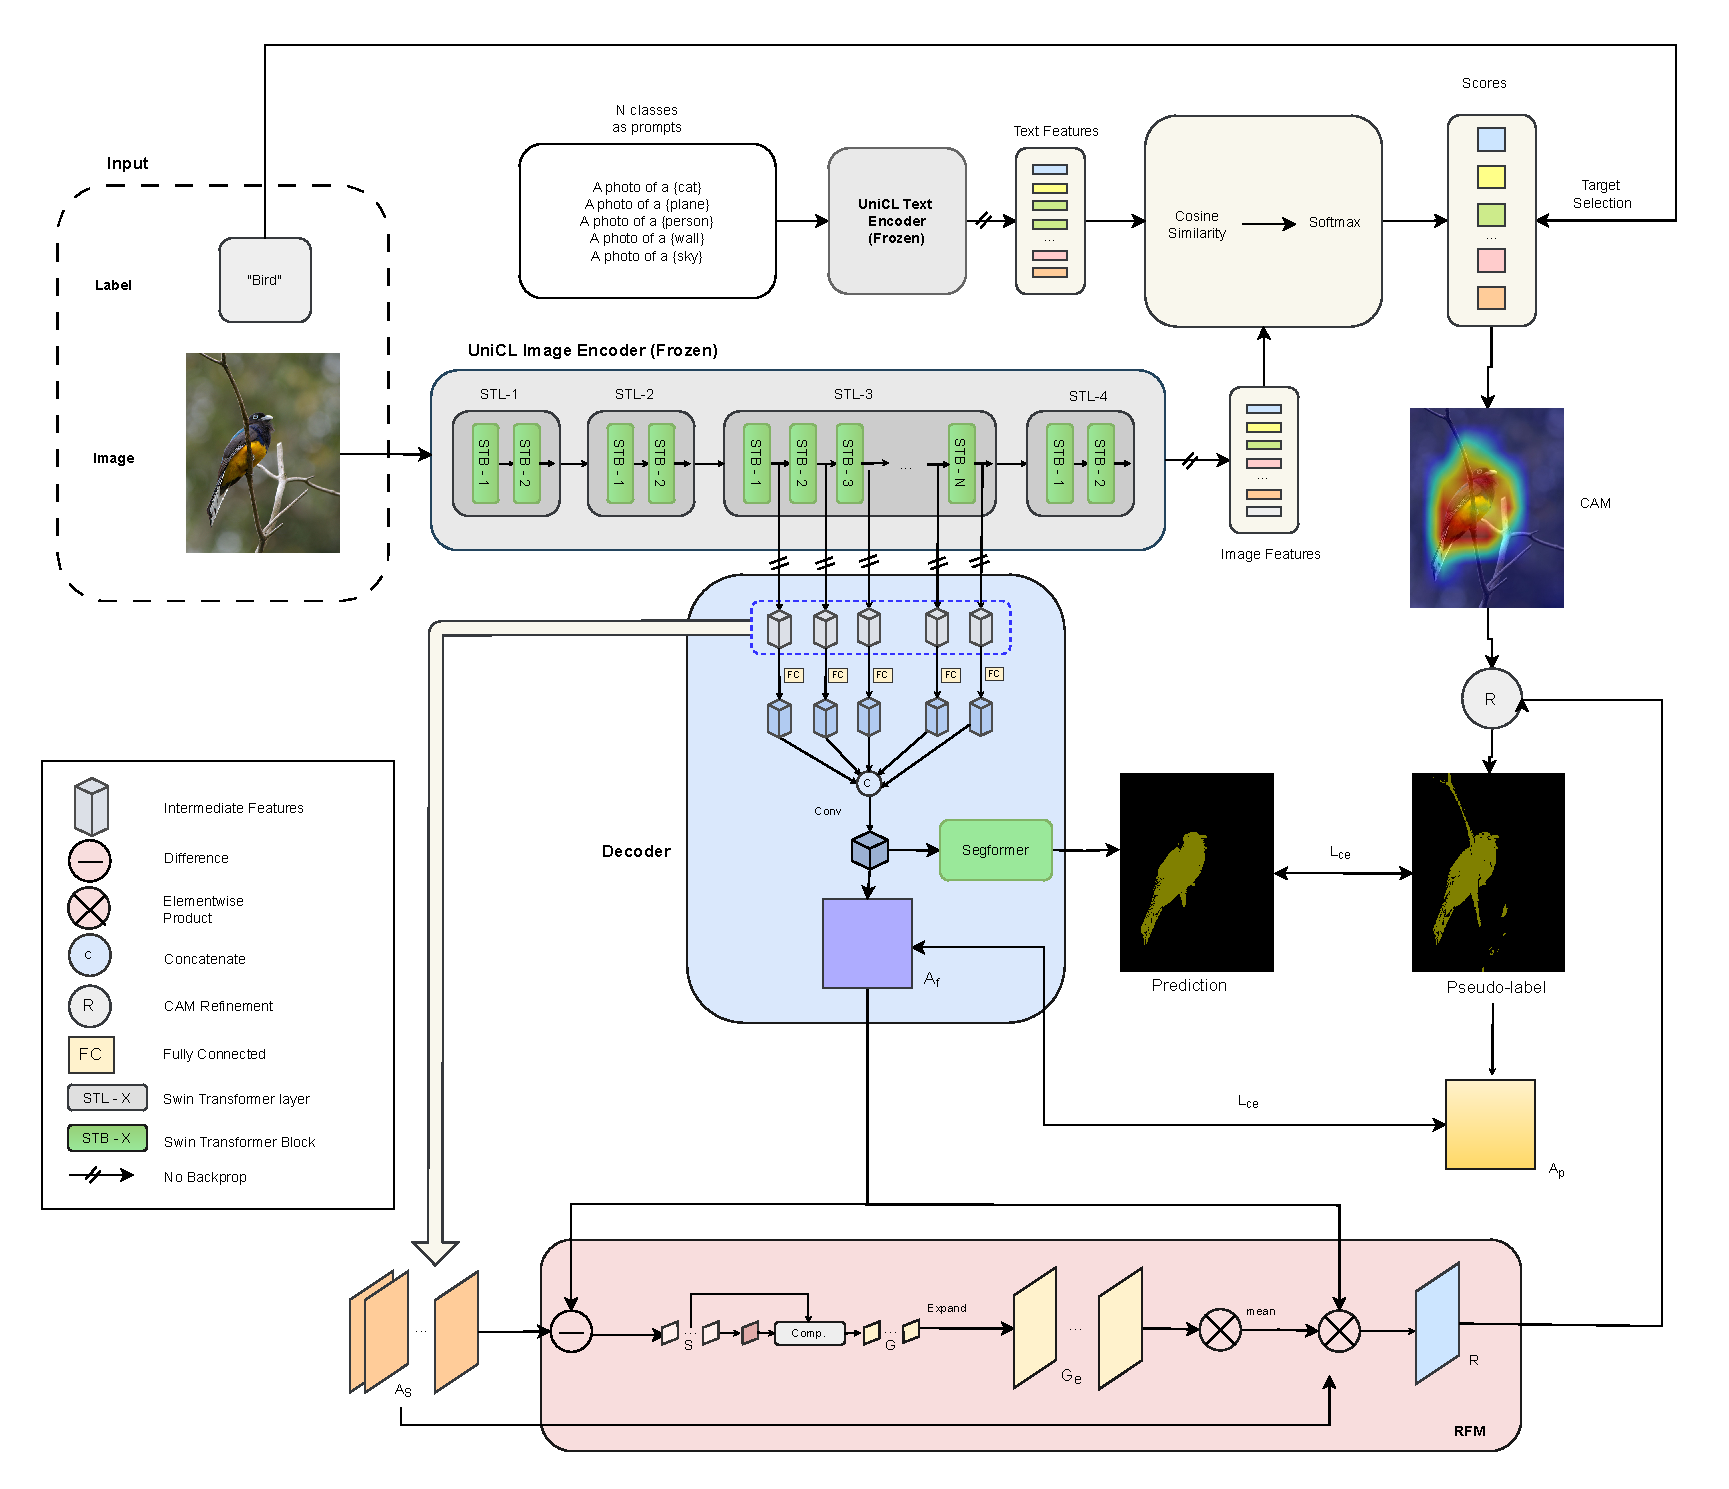
\includegraphics[width=0.98\textwidth, height = 1.05\textwidth]{figures/architecture}}
    \caption{Architecture of \textit{UniCL-AffSeg}}
    \label{fig:architecture}
\end{figure}

\begin{itemize}
    \item \textbf{Feature Extraction from Backbone}: The backbone network is responsible for generating Class Activation Maps (CAMs) from input images. We experiment with UniCL as the backbone due to its multi-modal capabilities and state-of-the-art performance in generating high-quality CAMs.
    \item \textbf{CAM Generation}: CAMs are generated using Grad-CAM techniques adapted for multi-modal models like UniCL. These CAMs highlight the regions of interest in the image for each class.
    \item \textbf{Segmentation Prediction}: The feature maps from the backbone are aggregated and passed through a decoder to produce segmentation predictions. The decoder employs multi-head transformer layers to refine the predictions.
    \item \textbf{CAM Refinement and Pseudo-Label Generation}: Initial CAMs are refined using affinity-based techniques and random walk propagation to generate high-quality pseudo-labels. These pseudo-labels serve as supervision for training the segmentation model.
    \item \textbf{Loss Function}: A combination of segmentation loss and affinity loss is used to optimize the model. The affinity loss ensures consistency between the affinity maps of the decoder and the pseudo-labels, while the segmentation loss aligns the predictions with the refined CAMs.
\end{itemize}

The proposed methodology integrates these components into a cohesive framework, enabling the generation of accurate segmentation maps from weak supervision signals. \autoref{fig:architecture} illustrates the overall architecture of the proposed methodology, highlighting the flow of data through each component.


\section{Feature Extraction from Backbone}
\label{sec:feature_extraction_from_backbone}

In weakly supervised semantic segmentation (WSSS), two components play a crucial role: class activation maps (CAMs) and pseudo labels. The CAMs are first generated from the backbone network, and these are subsequently used to construct pseudo labels. The pseudo labels then serve as supervision for training the segmentation head—or the full segmentation model in the case of a multi-stage approach. 

The accuracy of the initial CAMs directly affects the quality of the pseudo labels and, consequently, the performance of the segmentation model. To achieve robust feature representations, we employ UniCL \cite{vl_unicl}, a multi-modal contrastive learning model built upon the CLIP framework. In this section, we first introduce CLIP, outlining its core architecture and characteristics. We then discuss UniCL and its innovations over CLIP, followed by a description of the Swin Transformer backbone that underpins the image encoding process.

\subsection{Contrastive Language-Image Pre-Training (CLIP)}
\label{subsec:clip}

CLIP \cite{vl_clip} is a multi-modal learning framework that utilizes contrastive learning to align images and text within a shared embedding space. It is designed to acquire representations that generalize well across different tasks without the need for task-specific fine-tuning. By training on extensive datasets of image-text pairs, CLIP learns to capture meaningful associations between visual and textual modalities.

\subsection{CLIP Architecture}
\label{subsec:clip_architecture}

\subsubsection{CLIP Components}
CLIP comprises two principal components:

\begin{itemize}
    \item \textbf{Image Encoder}: Responsible for processing images and extracting feature representations. This typically involves a Swin Transformer, pooling layers, and additional modules to capture spatial hierarchies and relationships within image data.
    \item \textbf{Text Encoder}: Processes textual data and converts it into a format suitable for comparison with image features. It generally includes transformer layers and attention mechanisms to capture semantic relationships within the text.
\end{itemize}

CLIP is trained using a contrastive loss function that aligns image and text features in a shared embedding space. This enables the model to learn representations applicable to a variety of tasks, such as image classification, object detection, and image segmentation. In the context of this work, CLIP's capabilities are leveraged for weakly supervised semantic segmentation, which relies solely on image-level classification.

\subsection{Characteristics of CLIP}
\subsubsection{Multi-Modal Learning}
\label{subsec:multi_modal_learning}
Multi-modal learning involves integrating information from different modalities, such as images and text, to enhance model performance. By combining complementary cues from multiple sources, models can develop a deeper and more comprehensive understanding of the data. For instance, in classification tasks, leveraging both visual and textual data enables the model to capture more nuanced semantic relationships. A key advantage of this approach is the potential for zero-shot learning, where the model can recognize and classify images from previously unseen categories. This is accomplished by aligning visual features with corresponding textual descriptions, allowing the model to generalize beyond the training set. Such capabilities are particularly valuable, as classification often underpins many downstream applications.

\subsubsection{Contrastive Learning}
\label{subsec:contrastive_learning}
Contrastive learning is a self-supervised approach focused on learning representations by distinguishing between positive and negative pairs. The objective is to bring representations of related inputs (such as an image and its corresponding textual description) closer in a shared embedding space, while pushing apart representations of unrelated inputs. This is typically achieved using a contrastive loss function, which minimizes the distance between positive pairs and maximizes it for negative pairs. Such a strategy enables models to acquire robust, discriminative, and generalizable feature representations.

\subsubsection{Training Strategy}
\label{subsec:training_strategy}
The training strategy for multi-modal learning generally integrates both supervised and self-supervised techniques. Models are trained on large-scale datasets containing paired samples from different modalities, facilitating the learning of meaningful representations through methods such as contrastive learning. Data augmentation is commonly applied to enhance the diversity and robustness of the learned features, thereby improving the model's generalization to unseen data.

\subsubsection{Task-Agnostic Learning}
\label{subsec:task_agnostic_learning}
Task-agnostic learning refers to the development of representations that are not specialized for a single task but are applicable across a range of downstream applications. This is accomplished by focusing on learning generalizable features through training on diverse datasets and leveraging multi-modal information. As a result, models can adapt their learned representations to various tasks, including image classification, object detection, and image segmentation. This adaptability makes task-agnostic learning a valuable approach for constructing versatile and reusable models.

\subsection{Unified Contrastive Learning (UniCL)}
\label{subsec:unicl}

UniCL, or Unified Contrastive Learning \cite{vl_unicl}, is a multi-modal learning framework that extends the ideas of CLIP by unifying different contrastive learning strategies within a single architecture. This enables more effective and flexible learning from multiple modalities.

UniCL \cite{vl_unicl} is more than a straightforward extension of CLIP; it introduces several important innovations to improve both performance and adaptability.

A key feature of UniCL is its unified approach to contrastive learning, integrating image-label and text-label associations into a joint image-label-text space. This unified framework allows the model to leverage more positive pairs during training. While CLIP treats only the provided image-text pair as a positive match, UniCL recognizes that multiple text descriptions or images can correspond to the same category. For instance, both "a photo of a cat" and "a photo of a kitten" may be valid positive pairs for an image of a cat. UniCL's contrastive loss encourages the model to learn similarities across all features sharing the same category, resulting in a more comprehensive and robust shared representation space for images and text.

\subsubsection{Unified Image-Text-Label Contrast in UniCL}
\label{subsec:unified_image_text_label_contrast}

UniCL employs a bidirectional learning objective between image-text pairs:
\begin{equation} \label{eq:unified_image_text_label_contrast}
    \min_{\{\theta, \phi\}} \mathcal{L}_{\text{BiC}} = \mathcal{L}_{i2t} + \mathcal{L}_{t2i},
\end{equation}
where \(\mathcal{L}_{i2t}\) and \(\mathcal{L}_{t2i}\) are the image-to-text and text-to-image contrastive losses, respectively. And \(\theta\) and \(\phi\) are the parameters of the image and text encoders, respectively.

To align the representations of images and their corresponding textual descriptions within a batch, the image-to-text contrastive loss is formulated by \cite{vl_unicl}. This loss encourages the model to associate each image with all relevant text features that share the same class label, thereby strengthening the alignment between visual and textual modalities in the shared embedding space:
\begin{equation} \label{eq:unicl_image_to_text_contrastive_loss}
    \mathcal{L}_{i2t} = - \sum_{i \in \mathcal{B}} \frac{1}{|\mathcal{P}(i)|} \sum_{k \in \mathcal{P}(i)} 
    \log \frac{\exp(\tau \mathbf{u}_i^\top \mathbf{v}_k)}{\sum_{j \in \mathcal{B}} \exp(\tau \mathbf{u}_i^\top \mathbf{v}_j)},
\end{equation}
where $k \in \mathcal{P}(i) = \{k | k \in \mathcal{B}, y_k = y_i\}$, i.e., the set of all images in the batch that belong to the same class as image $i$.

Conversely, the text-to-image contrastive loss, which aligns each text feature in a batch with its corresponding image features, is formulated as:

\begin{equation} \label{eq:unicl_text_to_image_contrastive_loss}
    \mathcal{L}_{t2i} = - \sum_{j \in \mathcal{B}} \frac{1}{|\mathcal{P}(j)|} \sum_{k \in \mathcal{P}(j)} 
    \log \frac{\exp(\tau \mathbf{u}_k^\top \mathbf{v}_j)}{\sum_{i \in \mathcal{B}} \exp(\tau \mathbf{u}_i^\top \mathbf{v}_j)},
\end{equation}
where $k \in \mathcal{P}(j) = \{k \mid k \in \mathcal{B}, y_k = y_j\}$, i.e., the set of all text features in the batch that belong to the same class as text $j$.

\subsubsection{Comparison with CLIP}
\label{subsec:clip_vs_unicl}

In case CLIP, for an image, there is only one positive text feature. In other words, $\mathcal{P}(i) = {i} \in \mathcal{B}$; and $\mathcal{P}(j) = {j} \in \mathcal{B}$. So, the image-to-text contrastive loss is defined as:

\begin{equation} \label{eq:clip_image_to_text_contrastive_loss}
    \mathcal{L}_{i2t} = - \sum_{i \in \mathcal{B}} 
    \log \frac{\exp(\tau \mathbf{u}_i^\top \mathbf{v}_i)}{\sum_{j \in \mathcal{B}} \exp(\tau \mathbf{u}_i^\top \mathbf{v}_j)},
\end{equation}
where $i \in \mathcal{B}$ is the index of the image in the batch.

And the text-to-image contrastive loss is defined as:

\begin{equation} \label{eq:clip_text_to_image_contrastive_loss}
    \mathcal{L}_{t2i} = - \sum_{j \in \mathcal{B}} 
    \log \frac{\exp(\tau \mathbf{u}_j^\top \mathbf{v}_j)}{\sum_{i \in \mathcal{B}} \exp(\tau \mathbf{u}_i^\top \mathbf{v}_j)},
\end{equation}
where $j \in \mathcal{B}$ is the index of the text feature in the batch. 

The equations \ref{eq:unified_image_text_label_contrast}-\ref{eq:clip_text_to_image_contrastive_loss} are taken from \cite{vl_unicl}.

This means that $\mathcal{L}_{BiC}$ becomes CLIP training objective. The main property in \autoref{eq:unicl_text_to_image_contrastive_loss} is that for each image feature, any of the text features in the batch can be used as a positive pair. And so is the case for \autoref{eq:unicl_text_to_image_contrastive_loss}.

Second, UniCL replaces CLIP's ViT backbone with a Swin Transformer backbone. The Swin Transformer is a hierarchical vision transformer that captures both local and global information in images, making it more suitable for various vision tasks.

\subsection{Swin Transformer}
\label{subsec:swin_transformer}
The Swin Transformer \cite{transformer_swin} is a hierarchical vision transformer architecture that utilizes a shifted windowing mechanism to effectively capture both local and global image information. It is engineered for computational efficiency while delivering strong performance across a range of computer vision tasks. The model is organized into multiple stages, each comprising distinct transformer blocks, which enables the processing of images at varying resolutions and facilitates the extraction of multi-scale features.

\autoref{fig:swin_vs_vit_architecture} presents a comparative overview of the Swin Transformer and Vision Transformer (ViT) architectures. The principal difference between the two lies in their respective processing paradigms: the Swin Transformer adopts a hierarchical framework, operating on feature maps at multiple scales, whereas ViT processes the entire image globally at a single resolution. This hierarchical design empowers the Swin Transformer to simultaneously capture fine-grained local details and broader contextual information, making it particularly advantageous for applications that demand both.

Within the Swin Transformer, hierarchical feature maps are constructed by progressively merging image patches (shown in gray) at deeper network layers. Self-attention is computed exclusively within localized windows (indicated in red), resulting in linear computational complexity with respect to the input image size. This approach not only enhances efficiency but also renders the Swin Transformer highly suitable for dense prediction tasks, such as image segmentation and classification.

Conversely, conventional vision transformers like ViT generate feature maps at a single, lower resolution and apply self-attention globally, which incurs quadratic computational complexity relative to the input size. While global attention can be beneficial for certain tasks, it is less efficient for dense recognition scenarios compared to the localized attention employed by the Swin Transformer.

\begin{figure}[htbp]
    \centering
    \fbox{ % Draw a box around the entire figure
        \begin{minipage}{0.9\textwidth} % Adjust the width as needed
            \begin{subfigure}[b]{0.45\textwidth}
                \centering
                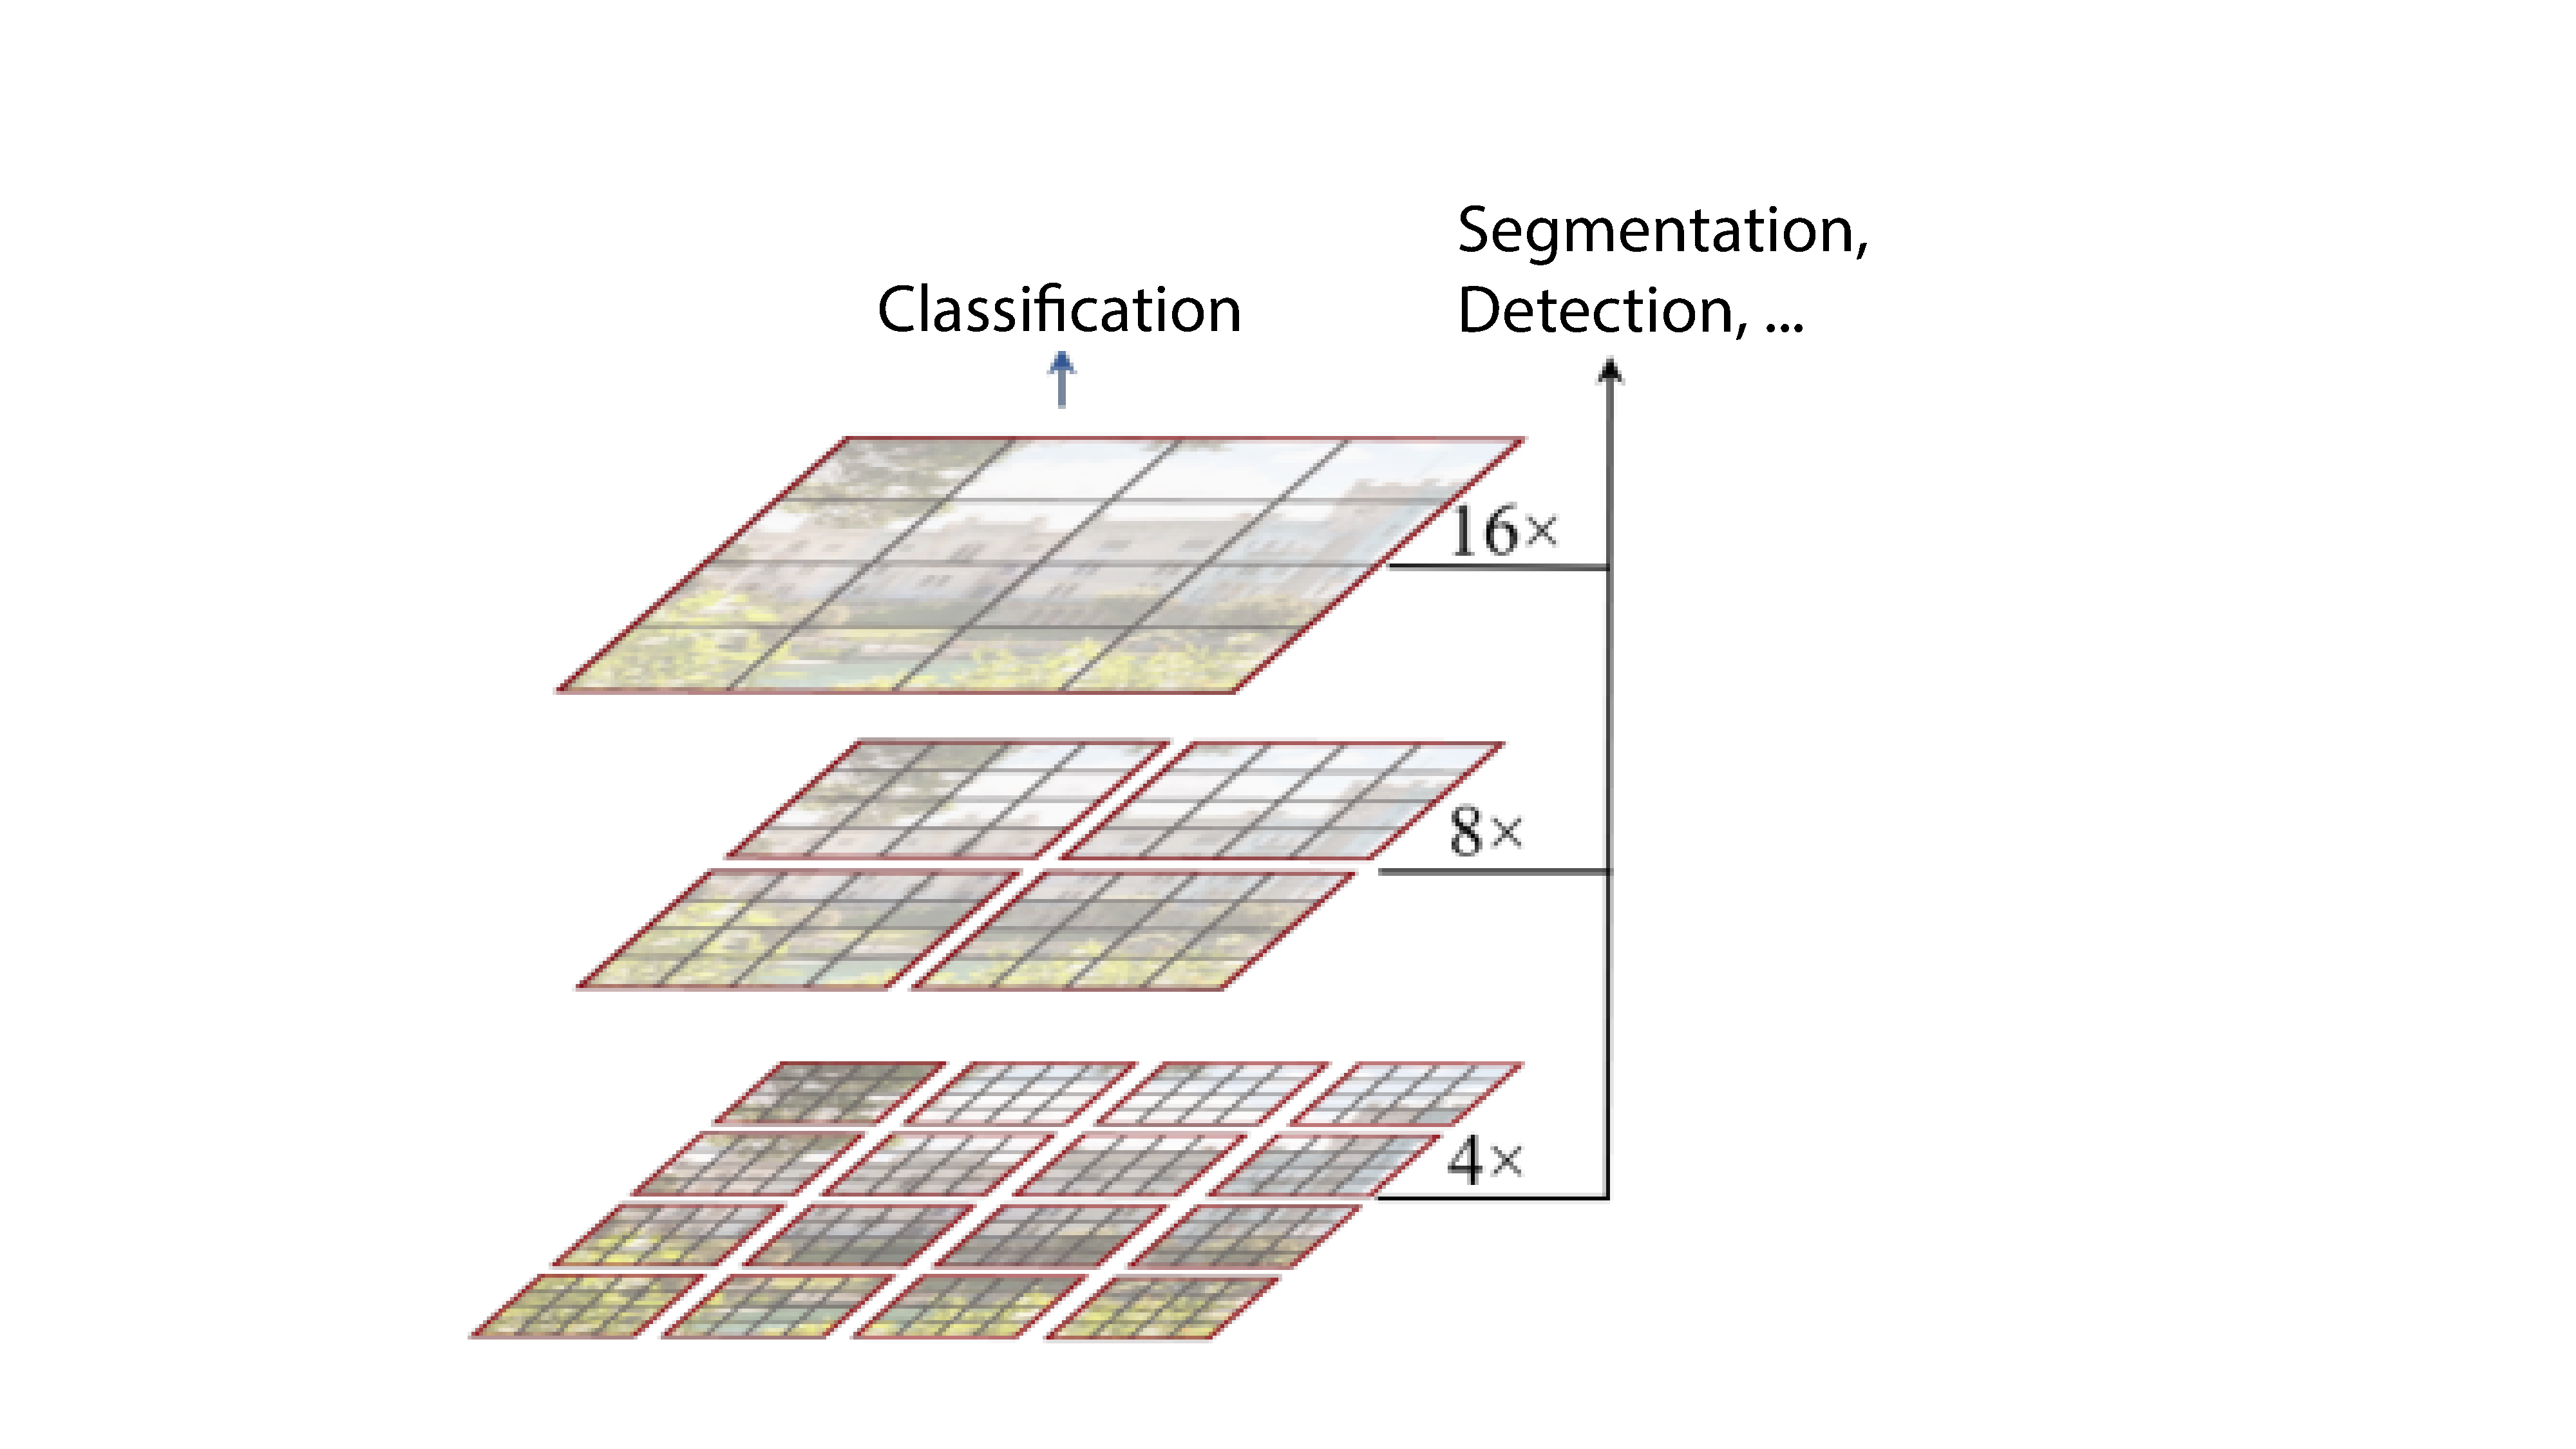
\includegraphics[width=\textwidth]{swin-vs-vit-archi-a.pdf}
                \caption{Swin Transformer}
                \label{fig:swin_transformer_data_flow}
            \end{subfigure}
            \hfill
            \begin{subfigure}[b]{0.45\textwidth}
                \centering
                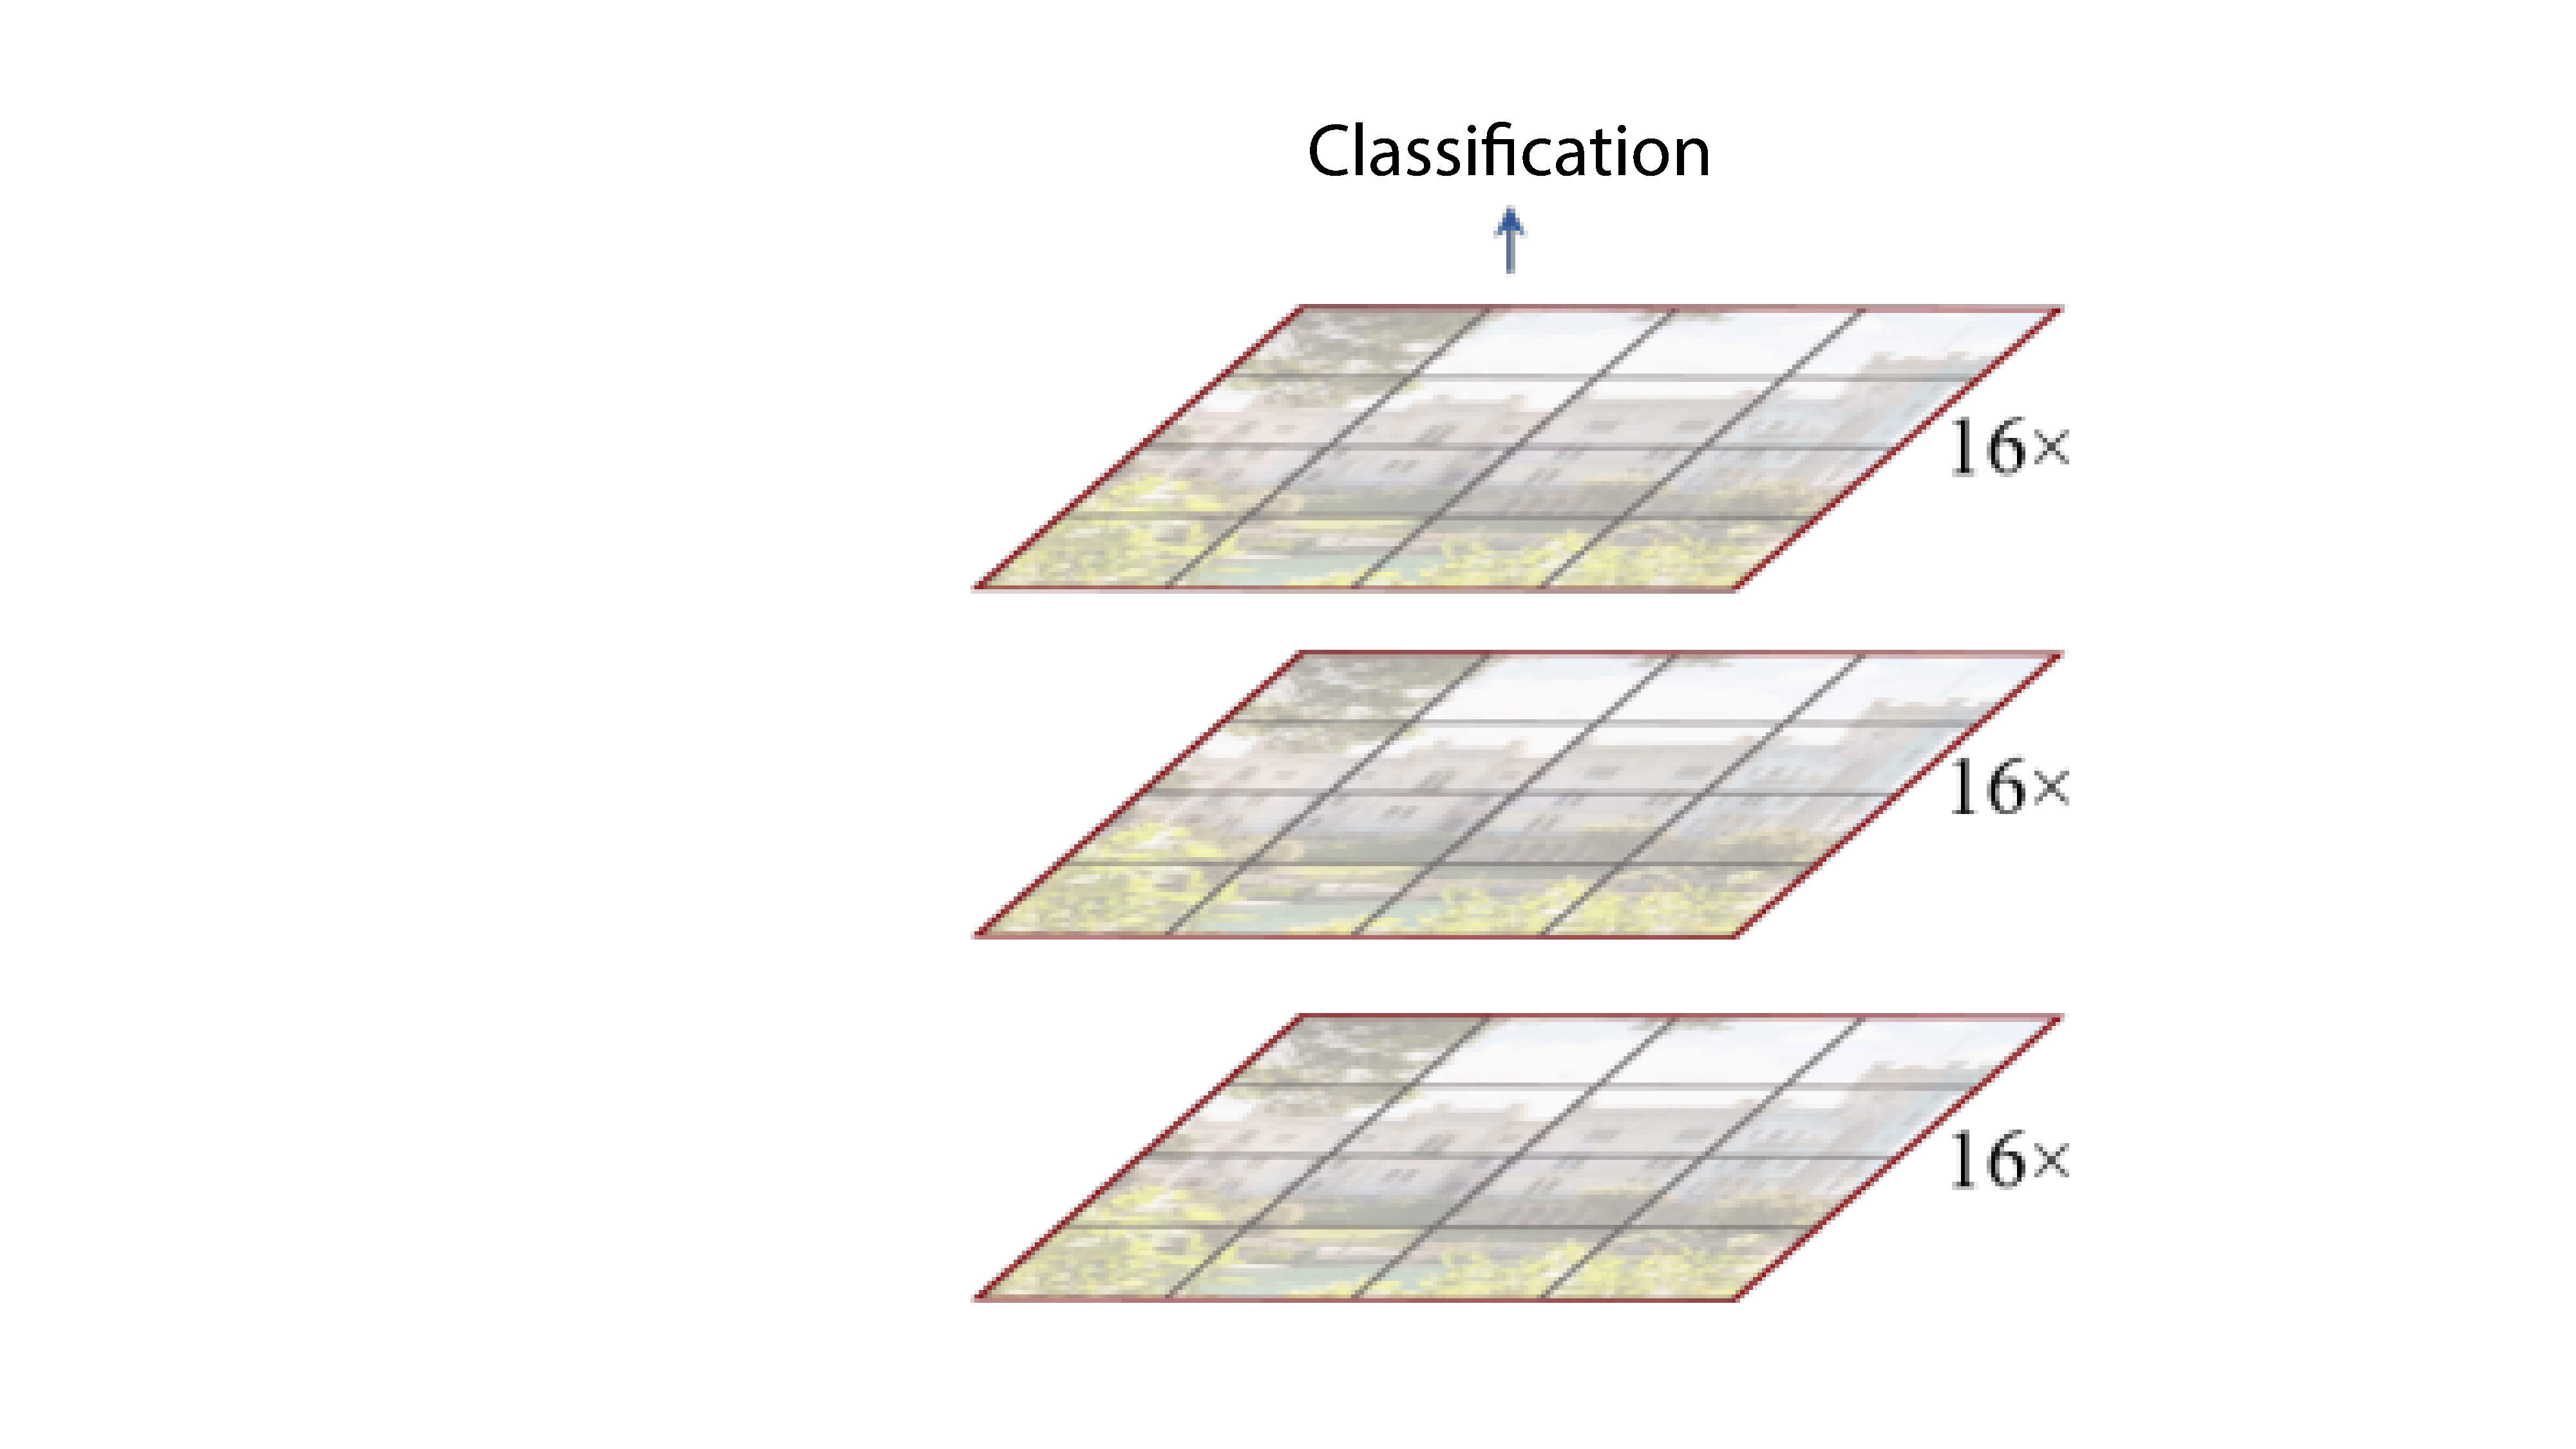
\includegraphics[width=\textwidth]{swin-vs-vit-archi-b.pdf}
                \caption{Vision Transformers}
                \label{fig:vit_data_flow}
            \end{subfigure}
        \end{minipage}
    }
    \caption{Comparison of Swin Transformer and ViT Architectures}
    \label{fig:swin_vs_vit_architecture}
\end{figure}

Owing to its hierarchical structure, the Swin Transformer is exceptionally well-suited for tasks that necessitate the integration of global context—essential for discerning the overall image structure—and local information, which is critical for identifying intricate features such as edges and textures. This makes it a compelling choice for image segmentation applications.

Furthermore, integrating the contrastive and multi-modal learning strengths of UniCL with the Swin Transformer's hierarchical design can significantly enhance the model's capacity to learn robust and discriminative representations from both visual and textual data. This synergy facilitates a more holistic understanding of multimodal inputs, thereby improving overall model performance.

With this foundational context established, the subsequent section details the proposed methodology, which comprises several core components: the backbone architecture, class activation map (CAM) generation, pseudo-label creation, segmentation prediction, and refinement. Each of these elements is integral to optimizing the model's effectiveness.


\begin{figure}[ht]
    \centering
    \setlength{\tabcolsep}{2pt} % adjust spacing
    \renewcommand{\arraystretch}{0.9}
    \fbox{ % Add border around the figure
        \begin{minipage}{0.7\textwidth}
            \centering
            % CAMs with class labels on the left
            \begin{tabular}{c c} % first column = label

            % Column headers
            (a) Original Image & (b) CAM \\
            [1mm]
            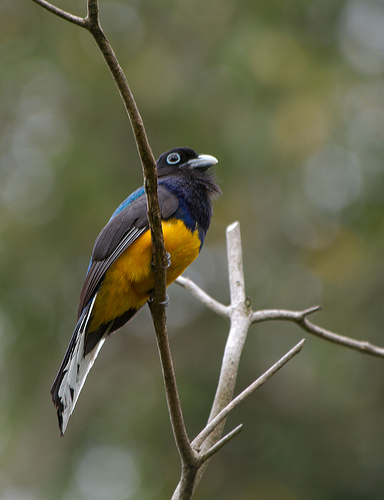
\includegraphics[width=0.45\textwidth,height=0.45\textwidth]{figures/originals/2009_004084.jpg}
            & 
            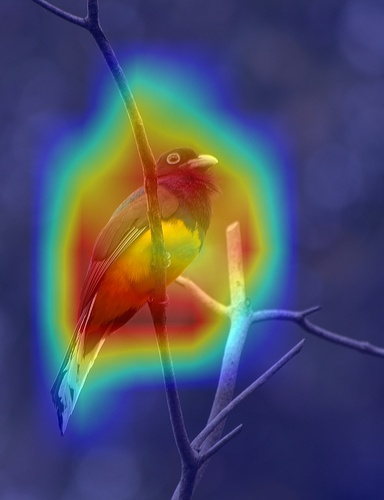
\includegraphics[width=0.45\textwidth,height=0.45\textwidth]{figures/test_cams/ours/2009_004084_2.jpg}
            \\
            \end{tabular}
        \end{minipage}
    }
    \caption{Original image and CAM generated by our method for class \textit{Bird}.}
    \label{fig:cam_examples}
\end{figure}

\section{CAM Generation}
\label{sec:cam_generation}

\autoref{fig:cam_generation_process_clip} shows the process of generating CAMs using CLIP/UniCL. We have used Grad-CAM. The process is similar to the method discussed in \autoref{subsec:grad_cam}, which is used to generate CAMs using CNN-based models.
 But there are some differences.

AS CLIP is a multi-modal model, the main classification task is to find similarity between the image and text. If we want to generate the CAM for $N$ classes, we need to provide $N$ text features as input. So, at the very beginning, we need to encode the text features using the CLIP text encoder, and store them.

An MLP layer takes the linear combination of the input features and the weights. We do the same thing when finding similarity score between the image and text features, take the linear combination of the image features and the text features. So, we can consider these text features as the "neuron weights" of the classifier head.

Then, we need to pass the image through the CLIP image encoder to get the feature maps. The rest of the process is the same as Grad-CAM. An example of the produced CAM for the \textit{Motorbike} class is shown in \autoref{fig:cam_examples}.


\begin{figure}[htbp]
    \centering
    \fbox{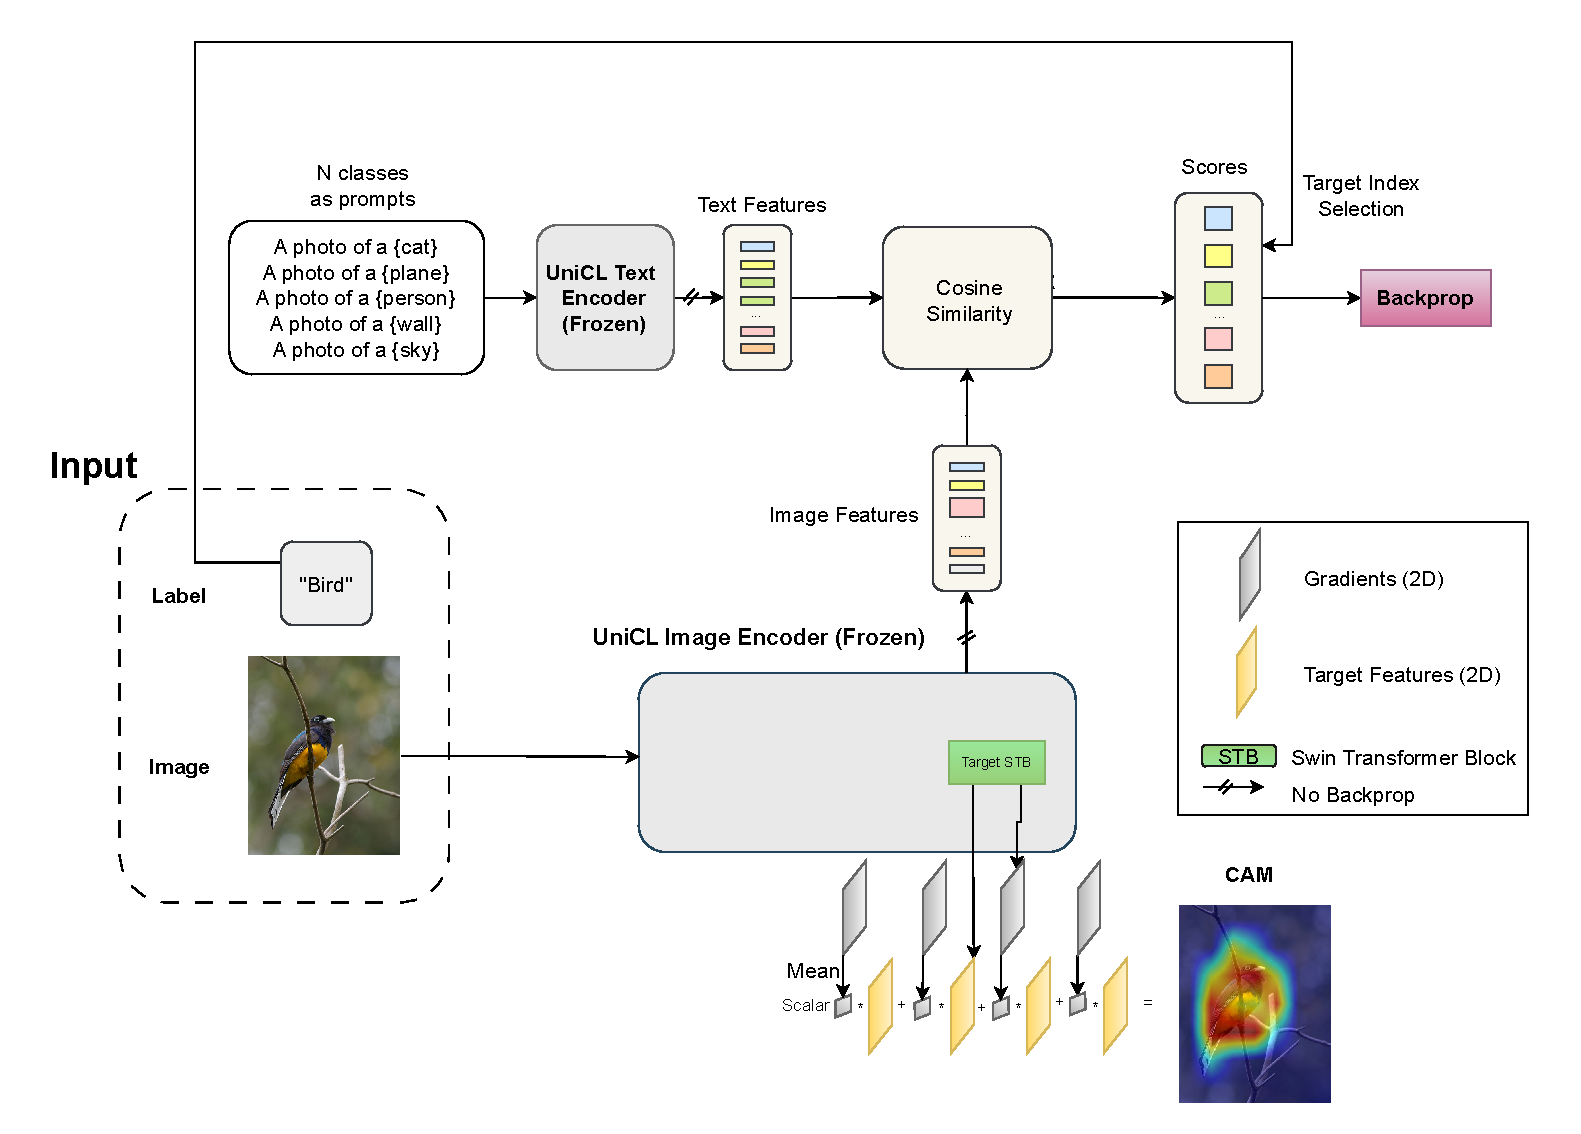
\includegraphics[width=0.8\textwidth]{methodology_cam.pdf}}
    \caption{CAM Generation Process using UniCL}
    \label{fig:cam_generation_process_clip}
\end{figure}

\section{Segmentation Prediction}
\label{sec:segmentation_prediction}
The segmentation prediction module is responsible for producing pixel-level class predictions for the input image. It comprises two primary stages: aggregation of encoder features and a decoder built with multi-head transformer layers. The design is inspired by the approach in \cite{wsss_frozen_clip}.

\subsection{Encoder Feature Aggregation}
\label{subsec:en_feature_agg}
In accordance with the methodology outlined in \cite{wsss_frozen_clip}, the feature representations extracted from each transformer block of the UniCL image encoder \cite{vl_unicl} are forwarded to the decoder for further processing. Denote the output feature map from the $l$-th transformer block as \( F_l^{\text{init}} \), where \( l = 1, \dots, N \). To harmonize the feature dimensions and enhance representational capacity, each \( F_l^{\text{init}} \) is individually transformed via a dedicated multilayer perceptron (MLP). Specifically, the transformation is defined as:
\begin{equation}
    F_l^{\text{new}} = W_{1}^{\text{fc}} \left( \text{ReLU} \left( W_{2}^{\text{fc}}(F_l^{\text{init}}) \right) \right),
\end{equation}
where \( W_{1}^{\text{fc}} \) and \( W_{2}^{\text{fc}} \) denote learnable fully connected layers, and \(\text{ReLU}(\cdot)\) represents the rectified linear unit activation function. This procedure ensures that the multi-scale features from different encoder stages are suitably projected for subsequent aggregation and decoding.


After that, all new feature maps \( F_l^{\text{new}} \) for \( l = 1, \dots, N \) are concatenated together, which are then processed by a convolution layer to generate a fused feature map \( F_u \):
\begin{equation}
    F_u = \text{Conv}\left( \text{Concat}\left[ F_1^{\text{new}}, F_2^{\text{new}}, \dots, F_N^{\text{new}} \right] \right),
    \tag{2}
\end{equation}

where \( F_u \in \mathbb{R}^{d \times h \times w} \), and \( d \), \( h \), and \( w \) represent the channel dimension, height, and width of the feature map, respectively. \(\text{Conv}(\cdot)\) is a convolutional layer, and \(\text{Concat}[\cdot]\) denotes the concatenation operation.


\subsection{Generating Final Prediction}
\label{subsec:decoder_final_pred}

Several sequential multi-head transformer layers are designed to generate the final prediction \( P \):
\begin{equation}
    \label{eq:prediction}
    P = \text{Conv}(\phi(F_u)) \uparrow,
\end{equation}
where \( P \in \mathbb{R}^{C \times H \times W} \), \( C \) is the number of classes including background, and \(\phi\) represents the sequential multi-head transformer blocks [12]. Each transformer block contains a multi-head self-attention module, a feed-forward network, and two normalization layers. The operator \(\uparrow\) denotes an upsampling operation to align the prediction map size with the original image.


\section{CAM Refinement and Pseudo-Label Generation}
\label{sec:refinement}
\subsection{Affinity based CAM refinement}  
The initial CAMs produced by the backbone tend to focus only on sparse, highly discriminative regions. These activations are often noisy and insufficient to be used directly as supervision. Therefore, a refinement module is required where the initial CAM is improved. The refined CAM is then used as a pseudolabel for supervision.  

The most common strategy for rectifying CAMs is by exploiting the feature relationships within the backbone that generates them. This is referred to as affinity-based CAM refinement, first introduced by \cite{wsss_affinitynet}. In transformer-based backbones, the attention maps naturally encode semantic-level affinities between tokens or patches. From these attention maps, an affinity matrix $A_f$ can be constructed and employed for CAM refinement via random walk propagation. In parallel, another affinity matrix, $A$, can be derived from the predicted pseudolabel produced by the decoder. The cross-entropy loss between these two affinity matrices is then incorporated into the training objective.  

However, in our case, the backbone responsible for generating the CAMs is \textbf{frozen}, meaning that its attention maps remain fixed and do not update during training. To address this limitation, Frozen CLIP \cite{wsss_frozen_clip} proposes utilizing the affinity derived from intermediate features of the encoder instead of directly relying on the backbone's frozen attention. The backbone attention maps are then used only to influence this encoder-derived affinity, producing a final refined matrix $R$, which is further transformed into a transition matrix $T$ for random walk propagation.  

\begin{figure}[t]
    \centering
    \fbox{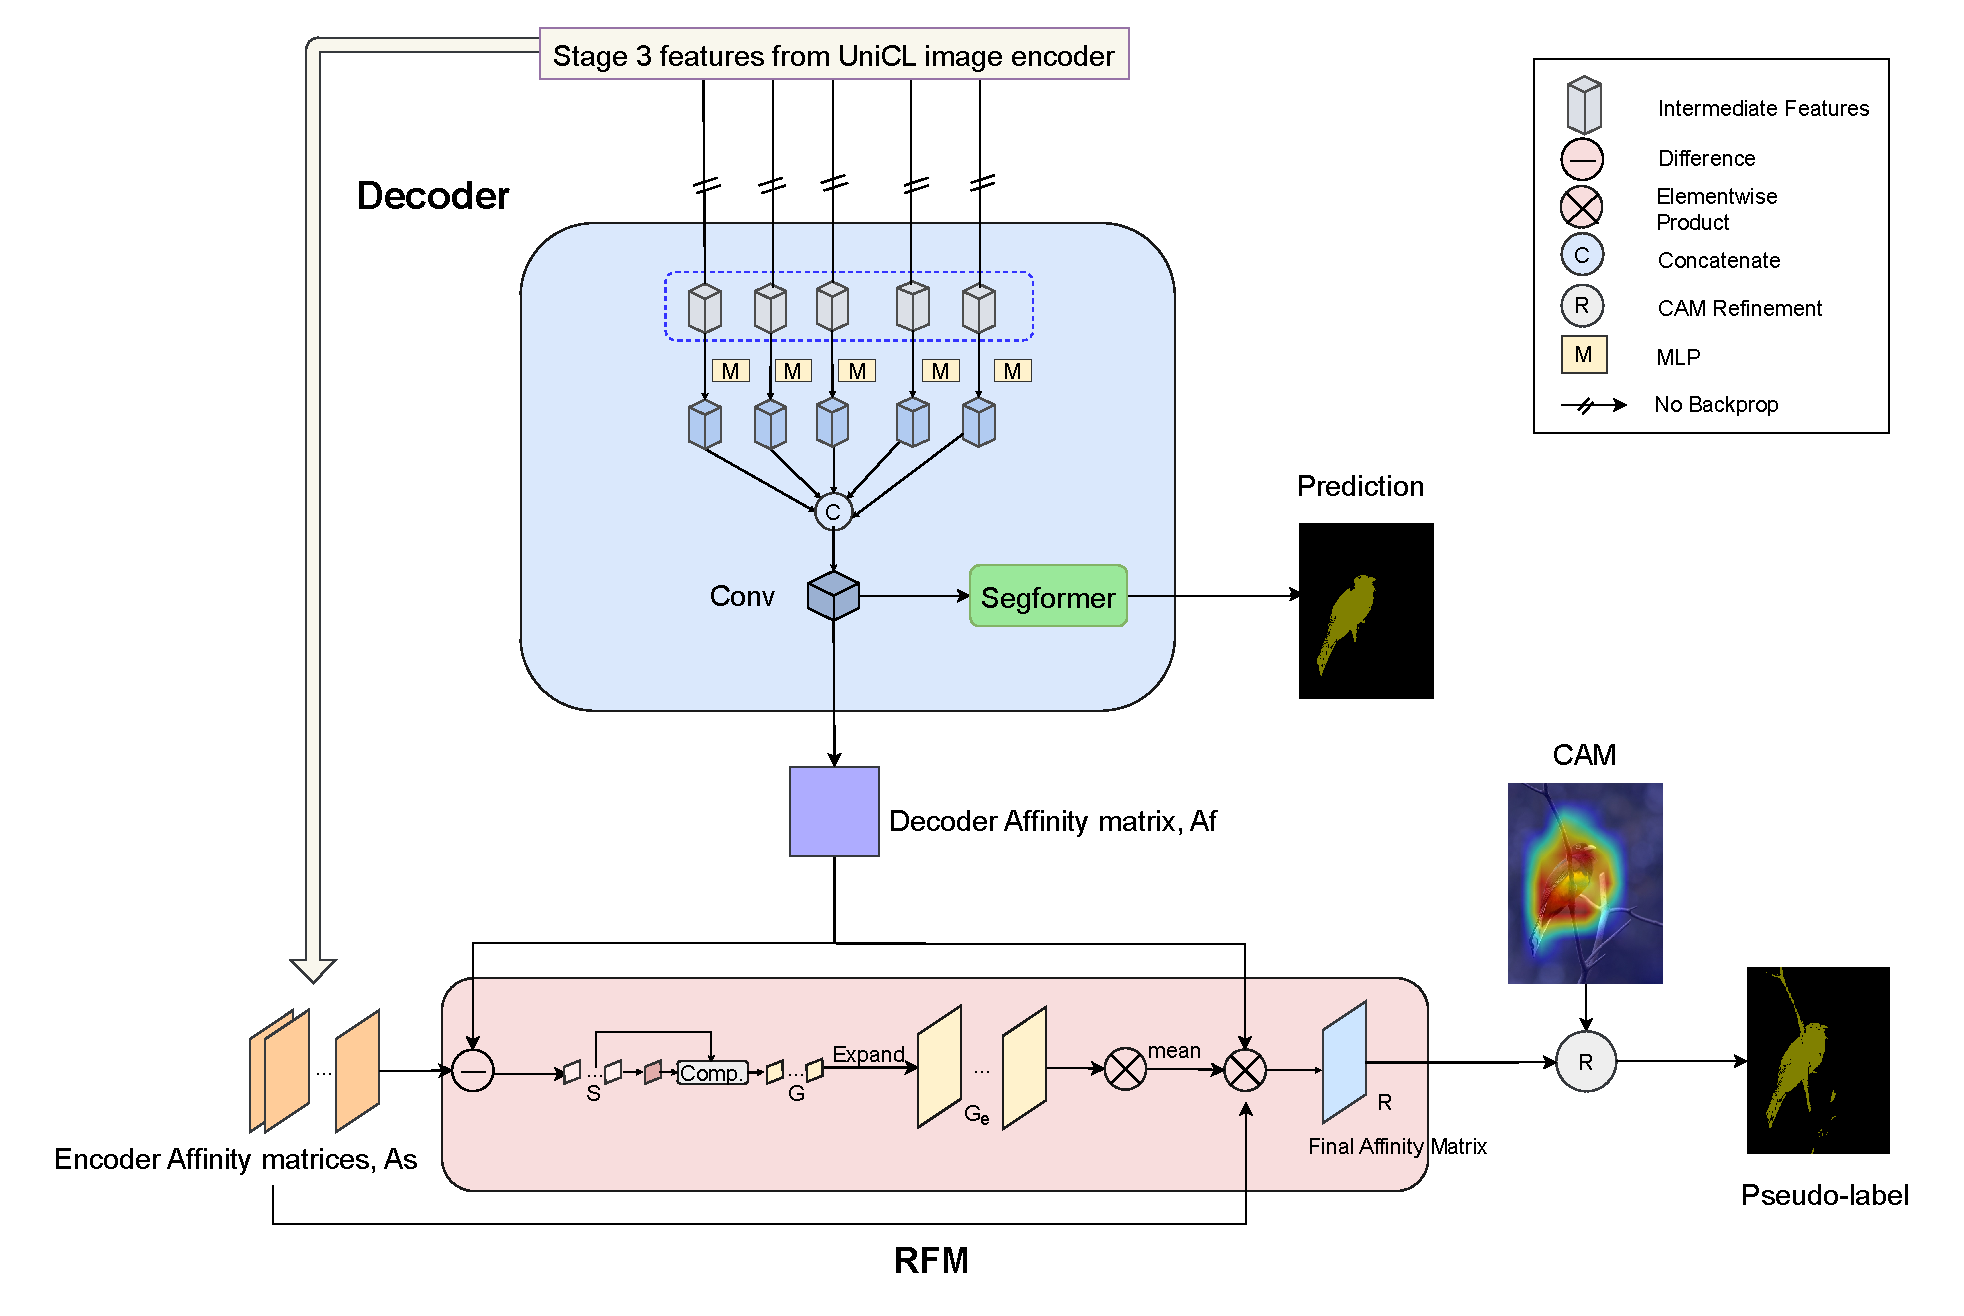
\includegraphics[width=0.9\textwidth]{figures/DecoderRFM}}
    \caption{Decoder and Refinement Module}
    \label{fig:decoder}
\end{figure}

In our setup, the UniCL backbone is based on the Swin Transformer, whose shifted-window design restricts the attention mechanism to \textbf{local regions}. Consequently, the attention maps fail to capture the \textbf{global semantic affinities} necessary for effective CAM propagation, and we could not use them directly for refinement. To overcome this, we compute affinities from the \textbf{intermediate feature maps of the Swin encoder}.  

Formally, let $f^{(k)} \in \mathbb{R}^{C \times L}$ denote the feature map from the $k$-th encoder block, where $C$ is the channel dimension and $L = h \times w$ represents the flattened spatial resolution. Each feature map is first normalized along the channel dimension:

\begin{equation}
\tilde{f}^{(k)}_i = \frac{f^{(k)}_i}{\| f^{(k)}_i \|_2}, \quad i = 1, \dots, L
\end{equation}

The affinity between spatial positions $i$ and $j$ within block $k$ is then computed as the dot-product similarity:

\begin{equation}
A^{(k)}_{ij} = \tilde{f}^{(k)}_i{}^\top \tilde{f}^{(k)}_j
\end{equation}

We compute such affinity matrices across multiple intermediate encoder blocks to capture complementary semantic relations at different abstraction levels. The resulting set of affinities is represented as:

\begin{equation}
\mathcal{A} = \{ A^{(1)}, A^{(2)}, \dots, A^{(N)} \}, \quad \mathcal{A} \in \mathbb{R}^{N \times hw \times hw}
\end{equation}

This multi-block affinity representation provides richer contextual cues for propagating and refining class activation maps.


\subsection{Extracting affinity map from the decoder}
\label{subsec:decoder_aff_mat}
Based on the feature map $F_u$ obtained from the decoder (as defined in Eq.~(2)), an affinity map is constructed as follows:

\begin{equation}
    \label{eq: A_f}
    A_f = \text{Sigmoid}(F_u^\top F_u),
\end{equation}

where $F_u \in \mathbb{R}^{d \times h \times w}$ is reshaped into a matrix of size $d \times hw$ before the computation. The $\text{Sigmoid}(\cdot)$ function ensures that the values in the resulting affinity map lie in the range $[0, 1]$. Consequently, the computed affinity map $A_f$ has the dimensions $\mathbb{R}^{hw \times hw}$. Here, $\top$ denotes the matrix transpose.

\subsection{Selecting affinity maps of the image encoder}
\label{subsec:att_map_encoder}
Following \cite{wsss_frozen_clip}, we extract all the affinity maps from the frozen CLIP image encoder, denoted as $\{A^l\}_{l=1}^N$, where each affinity map $A^l \in \mathbb{R}^{hw \times hw}$. To evaluate the reliability of each affinity map $A^l$, we compare it with the previously computed decoder affinity map $A_f$ using the following deviation score:

\begin{equation}
    S^l = \sum_{i=1}^{hw} \sum_{j=1}^{hw} \left| A_f(i, j) - A^l(i, j) \right|,
\end{equation}

where $S^l$ quantifies how much the affinity map (encoder) $A^l$ deviates from the reference affinity (decoder) $A_f$.  

Based on this score, we assign a binary weight $G^l$ to each affinity map:  

\begin{equation}
    G^l =
    \begin{cases}
        1, & \text{if } S^l < \dfrac{1}{N - N_0 + 1} \sum_{m=N_0}^N S^m, \\[8pt]
        0, & \text{otherwise}.
    \end{cases}
\end{equation}

Here, $G^l \in \{0,1\}$ is expanded to $G^l_e \in \mathbb{R}^{hw \times hw}$ for subsequent operations. The threshold is chosen as the average of the scores $\{S^m\}_{m=N_0}^N$ from the later layers of the encoder. If $S^l$ is lower than this threshold, the corresponding affinity map is considered reliable and retained ($G^l = 1$); otherwise, it is filtered out ($G^l = 0$).  

This selection mechanism ensures that only high-quality affinity maps consistent with the encoder-derived relationships are preserved, thereby improving the robustness of the CAM refinement process.  

\subsection{Utilizing the frozen encoder affinity maps}
\label{subsec: mul_attn_and_aff}
Using the affinity map $A_f$ and the filtered affinity maps of the encoder, we construct a refining map $R$ by weighing the decoder affinity matrix with the mean of the selected encoder affinity maps. This method of selection is adopted first by \cite{wsss_frozen_clip}. The equation is given as:

\begin{equation}
    R = A_f \odot \frac{ \sum_{l=1}^N G^l_e A^l}{N_m},
\end{equation}

where $\odot$ denotes element-wise multiplication, and $N_m$ is the number of valid encoder affinity maps that have passed the filtering stage, defined as:

\begin{equation}
    N_m = \sum_{l = N_0}^N G^l.
\end{equation}

Here, $G^l_e \in \mathbb{R}^{hw \times hw}$ is the expanded binary filter corresponding to $G^l$. The refining map $R$ effectively integrates the reliable encoder affinity maps weighted by the affinity map $A_f$, enhancing meaningful relationships while suppressing noisy or irrelevant information.

\subsection{Constructing the semantic transition matrix}
\label{subsec:trans_mat}
Now that we have the affinity matrix $R$, to apply the random walk propagation, we need to at first normalize the rows for converting it into a transition probability matrix. In addition, column normalization ensures consistency and symmetric behavior. Sinkhorn normalization \cite{math_sinkhorn} is thus used to convert $R$ into a double stochastic matrix $R_{\text{nor}}$.

Next, $R_{\text{nor}}$ is converted into a symmetric matrix by adding its transpose and normalizing the sum:

\[
    T = \frac{R_{\text{nor}} + R_{\text{nor}}^T}{2}, \quad \text{where} \quad R_{\text{nor}} = \text{Sinkhorn}(R)
\]

The matrix $T$ is now symmetric whose rows and columns are normalized. This is the transition probability matrix to be used for random walk.


\begin{figure}[tbp]
    \centering
    \fbox{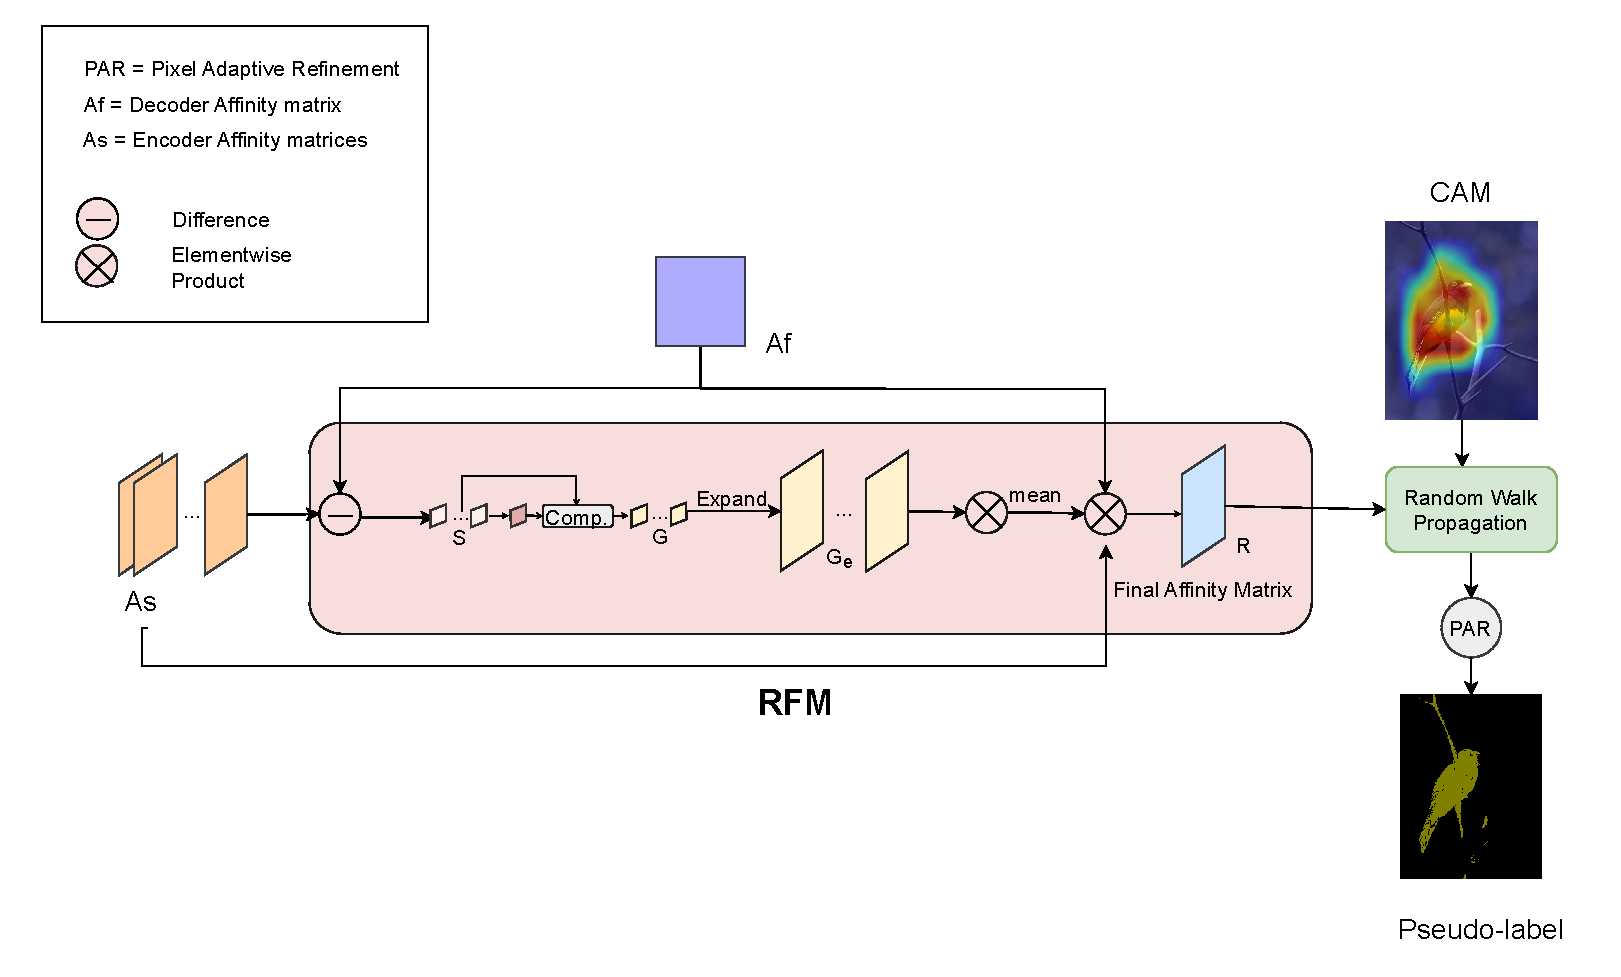
\includegraphics[width=0.95\textwidth]{figures/RFM}}
    \caption{CAM refinement by exploiting affinity map}
    \label{fig:refinement}
\end{figure}

\subsection{Random Walk Propagation}
\label{subsec:random_walk}

The refined class activation map (CAM) for a specific class $c$, denoted as $M^c_f$ is found by random walk propagation as follows:

\begin{equation}
    M_f^c = B^c \odot T^\alpha \cdot M_{\text{init}}^c
\end{equation}

where, $M^c_{\text{init}} \in \mathbb{R}^{hw \times 1}$ is the initial CAM for class $c$, reshaped into vector form. $T$ is the transition probability matrix, $\alpha$ is the hyperparameter that controls the strength of the refinement we want to apply. It is equivalent to the number of iterations of the random walk propagation. \( B^c \in \mathbb{R}^{1 \times hw} \) is the box mask obtained from the CAM of class \( c \), and \( \odot \) denotes the Hadamard product. This masking is needed to restrict the refining region spatially. It is obtained for each target class c by thresholding the CAM of this class by a constant. The connected regions of the mask map are found and covered by minimum rectangle bounding boxes. These boxes mask the affinity of distant pixels, preventing over-expansion.

Finally, the refined CAM $M^c_f$ is passed through an online post-processing module - specifically, the pixel-adaptive refinement module proposed in \cite{wsss_afa_affinity_from_attention}.

\subsection{Pixel Adaptive refinement module}
\label{subsec:par}
To ensure local consistency, pixel-adaptive convolution is introduced by \cite{wsss_afa_affinity_from_attention}. It uses local RGB and spatial information to define the low-level pair-wise semantic affinity of two pixels. Given an input image \( I \in \mathbb{R}^{h \times w \times 3} \), the pairwise affinities between two pixels at positions \((i, j)\) and \((k, l)\) is calculated as follows:

- \( \kappa^{\text{rgb}}_{ij,kl} \) measures color similarity (the closer the colors, the higher the affinity).

- \( \kappa^{\text{pos}}_{ij,kl} \) measures spatial closeness (pixels closer in space have higher affinity).

These are defined as:

\[
    \kappa^{\text{rgb}}_{ij,kl} = -\frac{\| I_{ij} - I_{kl} \|^2}{w_1 \sigma^2_{\text{rgb}}}, \quad
    \kappa^{\text{pos}}_{ij,kl} = -\frac{\| P_{ij} - P_{kl} \|^2}{w_2 \sigma^2_{\text{pos}}}
\]

Here:
- \( I_{ij} \) and \( P_{ij} \) are the RGB values and 2D spatial coordinates at pixel \((i, j)\),
- \( \sigma_{\text{rgb}} \) and \( \sigma_{\text{pos}} \) are the standard deviations of color and position differences,
- \( w_1 \) and \( w_2 \) are weights that control smoothness.

Then, the affinity kernel \( \kappa_{ij,kl} \) for each pixel pair is computed by applying a softmax to normalize both terms across the local neighborhood \( \mathcal{N}(i, j) \), and combining them:

\[
    \kappa_{ij,kl} = \frac{ \exp(\kappa^{\text{rgb}}_{ij,kl}) }{ \sum\limits_{(x, y) \in \mathcal{N}(i, j)} \exp(\kappa^{\text{rgb}}_{ij,xy}) }
    + w_3 \cdot \frac{ \exp(\kappa^{\text{pos}}_{ij,kl}) }{ \sum\limits_{(x, y) \in \mathcal{N}(i, j)} \exp(\kappa^{\text{pos}}_{ij,xy}) }
\]

Here, \( w_3 \) is a weight to balance the influence of the position term.

This affinity kernel is used to iteratively refine a CAM \( M \in \mathbb{R}^{h \times w \times C} \). At iteration \( t \), each pixel value \( M^t_{i,j,c} \) for class \( c \) is updated by aggregating class scores from neighboring pixels weighted by the affinity:

\begin{equation}
    M^t_{i,j,c} = \sum_{(k, l) \in \mathcal{N}(i, j)} \kappa_{ij,kl} \cdot M^{t-1}_{k,l,c}
\end{equation}


The neighborhood \( \mathcal{N}(i, j) \) is defined as the 8-connected neighbors (i.e., a \(3\times{3}\) window) with multiple dilation rates  allowing the refinement to capture both local and semi-local context.

\begin{figure}[ht]
    \centering
    \setlength{\tabcolsep}{2pt} % adjust spacing
    \renewcommand{\arraystretch}{0.9}
    \fbox{ % Add border around the figure
        \begin{minipage}{0.7\textwidth}
            \centering
            % CAMs with class labels on the left
            \begin{tabular}{c c} % first column = label

            % Column headers
            (a) Ground Truth & (b) Pseudolabel \\
            [1mm]
            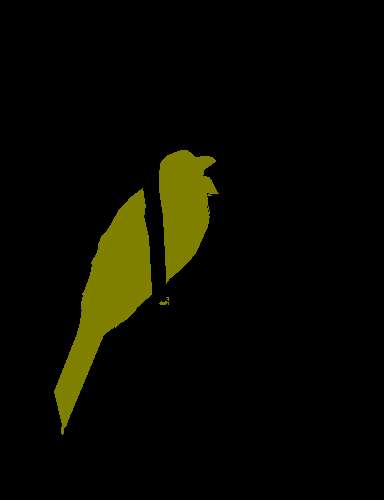
\includegraphics[width=0.4\textwidth,height=0.4\textwidth]{figures/colored_gts/2009_004084}
            & 
            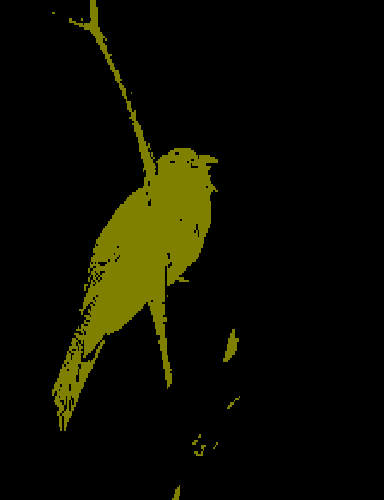
\includegraphics[width=0.4\textwidth,height=0.4\textwidth]{figures/test_labels/ours/2009_004084_[2]}
            \\
            \end{tabular}
        \end{minipage}
    }
    \caption{Ground Truth Label and Pseudolabel generated by our method for class \textit{Bird}.}
    \label{fig:pseudolabel_examples}
\end{figure}


\subsection{Pseudo-Label Generation}
\label{subsec:pseudo_label_generation}
The refined CAMs are used to generate the pseudo-labels or segmentation labels, which assign a class label to each pixel (patch),
\begin{equation}
    M_p(x, y) = \arg\max_{c \in \{1, \ldots, C\}} M_c(x, y)
\end{equation}
where \( M_c \in \mathbb{R}^{h \times w} \) is the refined CAM and \( M_p \in \mathbb{R}^{h \times w} \) is the pseudo-label.
The generated pseudo-labels are used as supervision for the segmentation network.



\section{Loss Function}
\label{subsec:loss_func}

The loss function defined by \cite{wsss_frozen_clip}:
\begin{equation}
    \mathcal{L} = \mathcal{L}_{seg} + \lambda \mathcal{L}_{aff}
\end{equation}

where, $\mathcal{L}_{aff}$ is the affinity loss and $\mathcal{L}_{seg}$ is the segmentation loss. $\lambda$ is the weighting parameter.
\subsection{Affinity Loss}
\label{aff_loss}

In the refinement module, we used the affinity map of the decoder features, $A_f$ (\autoref{eq: A_f}). The quality of the final pseudolabel directly depends on it. We need to ensure that the pairwise affinity of the pseudolabel matches the pairwise affinity of the decoder output, because that is what the random walk propagation implies.
We compute the affinity labels for the predicted pseudolabel as follows:

\begin{equation}
    A_p = O_h(M_p)^TO_h(M_p)
\end{equation}
where $O_h(.)$ is the one-hot encoding of $M_p$, and $A \in \mathbb{R}^{hw \times hw}$  is the affinity label.
. This means that the value of $A_p(i,j)$ will be 1 for the $(i,j)$ pair which have the same class label, and 0 otherwise. The affinity loss is the Cross-Entropy Loss of $A_f$ and $A_p$:
\begin{equation}
    \mathcal{L}_{aff} = \mathcal{L}_{ce}(A_f, A_p)
\end{equation}

\subsection{Segmentation Loss}
\label{seg_loss}
We obtain the segmentation prediction, $P$, from the decoder (\autoref{eq:prediction}). As we are using the refined CAM or pseudolabel, $M_p$ as supervision, the segmentation loss is computed:

\begin{equation}
    \mathcal{L}_{seg} = \mathcal{L}_{ce}(P, M_p \uparrow)
\end{equation}

where \( L_{ce} \) is the cross-entropy loss, and \( M_p{\uparrow} \in \mathbb{R}^{H \times W} \). $H$ and $W$ are the original height and width of the image respectively.




\chapter{Result Analysis}
\label{sec:result_analysis}

% \begin{figure}[htbp]
%     \centering
%     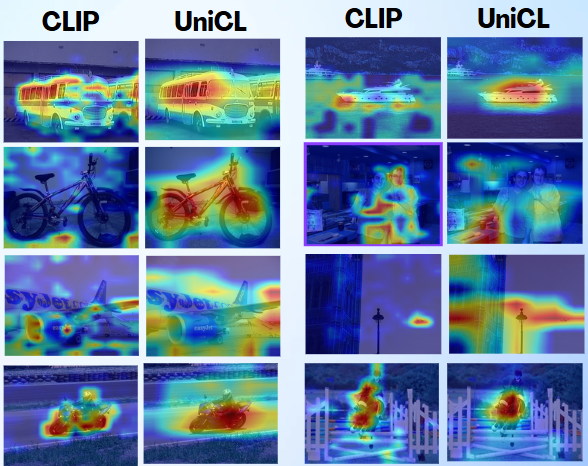
\includegraphics[width=0.8\textwidth]{clip_vs_unicl.png}
%     \caption{Quantitative analysis of CAMs produced by CLIP and Swin}
%     \label{fig:cam_results}
% \end{figure}

% \autoref{fig:cam_results} shows the comparison of the CAMs generated by CLIP \cite{vl_clip} and UniCL \cite{vl_unicl} on the Pascal VOC 2012 dataset. The results indicate that UniCL produces more accurate and detailed CAMs compared to CLIP. You can see the bicycle in second row, first two columns, CLIP even failed to detect it, while UniCL was localize it very well. The same is true for third and fourth columns of the same row, where CLIP failed to highlight the boat, but UniCL did.

% Additionally, we can see in all the images that, the CAMs produced by CLIP are discontinuous and sparse, while the CAMs produced by UniCL are more continuous and dense. This indicates that UniCL is better at capturing the global context of the image.

% However, we also observed that the CAMs produced by UniCL are still not perfect. It produces a lot of false positives, for example, look at the third row, last column, where it was supposed highlight an aeroplane, but it also highlighted the background. Also in some cases, like the last row, CLIP was able to trace the object boundary with better detail. This indicates that there is still room for improvement in the CAM generation process.

\section{Data and Experimental Setup}
\label{subsec:data_and_experimental_setup}

We conducted our experiments on the \textbf{Pascal VOC 2012} dataset \cite{dataset_pascal_voc}, 
which contains 20 object categories and one background class. 
The dataset is split into 1,464 training images, 1,449 validation images, 
and 1,456 test images. Since the test set does not provide ground truth 
annotations, we used the training set for model training and the validation 
set for performance evaluation.

All experiments were implemented in the \textbf{PyTorch} framework and executed 
on a single \textbf{NVIDIA Tesla T4 GPU} with \textbf{16 GB of memory}, 
provided by Google Colab (free tier). During training, images were randomly 
resized within the range of 512--2048 pixels, rescaled by factors between 
0.5 and 2.0, and cropped to a fixed size of 224.

Optimization was performed using the \textbf{AdamW} optimizer with a learning 
rate of $5 \times 10^{-5}$, $\beta_1 = 0.9$, $\beta_2 = 0.999$, and a weight 
decay of 0.01. We trained the models for \textbf{30,000 iterations} with an 
effective batch size of 8 (per-GPU batch size of 4 with gradient accumulation 
steps of 2). A linear warmup strategy was applied during the first 500 iterations 
with a warmup ratio of $10^{-3}$. The best-performing checkpoints were selected 
based on validation set performance.



\section{Quantitative Results}
\label{subsec: Quantitative Results}
We compared the performance of our proposed method with the baseline method CLIP \cite{wsss_frozen_clip} on the Pascal VOC 2012 dataset. The results are shown in Table \ref{tab:quantitative_results}. Our proposed method outperforms the baseline method by a significant margin, achieving a mIoU of 55.4\% compared to 47.5\% for the baseline method. This demonstrates the effectiveness of our proposed method in generating accurate CAMs for weakly supervised semantic segmentation.

\begin{table}[ht]
    \centering
    \renewcommand{\arraystretch}{1.2}
    \setlength{\tabcolsep}{6pt}
    \begin{tabular}{l c c c c}
        \hline
        Method                                                               & Backbone   & Sup. & val           & test          \\
        \hline
        \multicolumn{5}{c}{\textit{multi-stage weakly supervised approaches}}                                                    \\
        RCA$_{\text{CVPR'22}}$~\cite{wsss_RCA}             & ResNet101  & I+S  & 72.2          & 72.8          \\
        L2G$_{\text{CVPR'22}}$~\cite{wsss_L2G}             & ResNet101  & I+S  & 72.1          & 71.7          \\
        Mat-label$_{\text{ICCV'23}}$~\cite{wsss_MatLabel}  & ResNet101  & I+S  & 73.3          & \textbf{74.0} \\
        S-BCE$_{\text{ECCV'22}}$~\cite{wsss_s_bce}         & ResNet38   & I+S  & 68.1          & 70.4          \\
        RIB$_{\text{NeurIPS'21}}$~\cite{wsss_rib}          & ResNet38   & I    & 68.3          & 68.6          \\
        W-OoD$_{\text{CVPR'22}}$~\cite{wsss_ood}      & ResNet101  & I    & 69.8          & 69.9          \\
        ESOL$_{\text{NeurIPS'22}}$~\cite{wsss_esol}   & ResNet101  & I    & 69.9          & 69.3          \\
        VML$_{\text{IJCV'22}}$~\cite{wsss_vml}        & ResNet101  & I    & 70.6          & 70.7          \\
        AETF$_{\text{ECCV'22}}$~\cite{wsss_aetf}      & ResNet38   & I    & 70.9          & 71.7          \\
        MCTformer$_{\text{CVPR'22}}$~\cite{wsss_MCTformer} & ViT+Res38  & I    & 70.4          & 70.0          \\
        CDL$_{\text{IJCV'23}}$~\cite{wsss_cdl}        & ResNet101  & I    & 72.4          & 72.2          \\
        ACR$_{\text{CVPR'23}}$~\cite{wsss_acr}        & ViT        & I    & 72.4          & 72.4          \\
        BECO$_{\text{CVPR'23}}$~\cite{wsss_beco}      & MIT-B2     & I    & 73.7          & 73.5          \\
        FPR$_{\text{ICCV'23}}$~\cite{wsss_fpr}        & ResNet101  & I    & 70.0          & 70.6          \\
        USAGE$_{\text{ICCV'23}}$~\cite{wsss_usage}    & ResNet38   & I    & 71.9          & 72.8          \\
        CLIMS$_{\text{CVPR'22}}$~\cite{wsss_clims}    & ViT+Res101 & I+L  & 70.4          & 70.0          \\
        CLIP-ES$_{\text{CVPR'23}}$~\cite{wsss_clip_es}                       & ViT+Res101 & I+L  & \textbf{73.8} & 73.9          \\
        \hline
        \multicolumn{5}{c}{\textit{single-stage weakly supervised approaches}}                                                   \\
        1Stage$_{\text{CVPR'20}}$~\cite{wsss_single_stage}                   & ResNet38   & I    & 62.7          & 64.3          \\
        RRM$_{\text{AAAI'20}}$~\cite{wsss_reliability_does_matter}           & ResNet38   & I    & 62.6          & 62.9          \\
        AA\&AR$_{\text{ACMMM'21}}$~\cite{wsss_aaar}                                 & ResNet38   & I    & 63.9          & 64.8          \\
        SLRNet$_{\text{IJCV'22}}$~\cite{34}                                  & ResNet38   & I    & 67.2          & 67.6          \\
        AFA$_{\text{CVPR'22}}$~\cite{39}                                     & MIT-B1     & I    & 66.0          & 66.3          \\
        TSCD$_{\text{AAAI'23}}$~\cite{53}                                    & MIT-B1     & I    & 67.0          & 67.5          \\
        ToCo$_{\text{CVPR'23}}$~\cite{40}                                    & ViT        & I    & 71.1          & 72.2          \\
        \hline
        ours-WeCLIP (w/o CRF)                                                & ViT        & I+L  & 74.9          & 75.2          \\
        ours-WeCLIP (w/ CRF)                                                 & ViT        & I+L  & \textbf{76.4} & \textbf{77.2} \\
        \hline
    \end{tabular}
    \caption{Comparison of multi-stage and single-stage weakly supervised approaches.}
    \label{tab:quantitative_results}
\end{table}

\section{Qualitative Analysis}
\label{sec:qualitative_analysis}

We present qualitative comparisons of our UniCL-AffSeg framework against the WeCLIP baseline and ground truth annotations on selected Pascal VOC 2012 images. Both class activation maps (CAMs) and pseudo-labels are visualized to highlight differences in object localization, boundary delineation, and overall mask quality.

% \subsection{Selection of Examples}
% The images were chosen to represent a variety of scenarios, including: 
% \begin{itemize}
%     \item \t	\textbf{Easy cases:} Large, isolated objects where CAMs are expected to cover most of the object region.
%     \item \t	\textbf{Challenging cases:} Small objects, occlusions, or cluttered backgrounds where weakly supervised CAMs often fail to capture complete object extents.
% \end{itemize}

% \subsection{Visualization Layout}
% Figure~\ref{fig:qualitative_comparison} shows the qualitative results in a structured grid. 
% The first row presents the input image, ground truth, WeCLIP CAM, and our CAM, while the second row shows the corresponding pseudo-labels generated by WeCLIP and our method. This layout allows a direct comparison of both intermediate activations and the resulting segmentation masks.


\begin{figure}[ht]
  \centering
  \setlength{\tabcolsep}{2pt} % adjust spacing
  \renewcommand{\arraystretch}{0.9}

  % Wrap the table in a colored box (requires \usepackage{tcolorbox})
  \begin{tcolorbox}[colframe=black!60, colback=white, boxrule=0.8pt, arc=2pt, left=2pt, right=2pt, top=2pt, bottom=2pt]
    \centering
    % CAMs with class labels on the left
    \begin{tabular}{m{3cm} c c c} % first column = label

      % Column headers
       & (a) Input                                                    & (b) WeCLIP & (c) Ours
      \\
      [1mm]

      {\textbf{Cat}}
       & 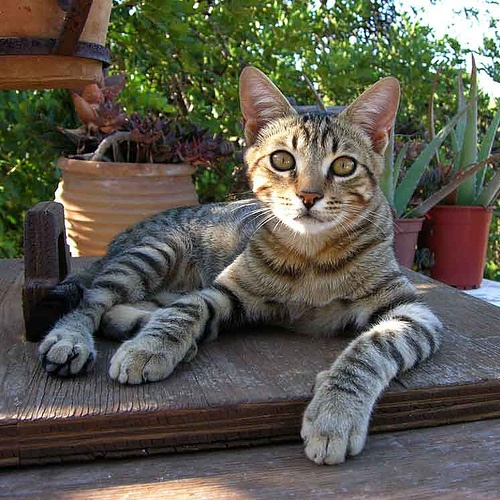
\includegraphics[width=0.20\textwidth,height=0.20\textwidth]
      {figures/originals/2007_003778}
       & 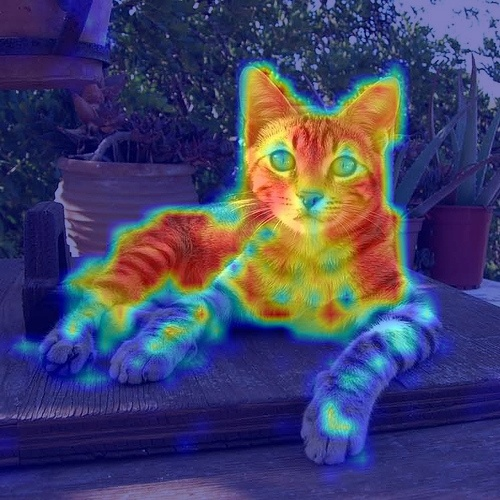
\includegraphics[width=0.20\textwidth,height=0.20\textwidth]
      {figures/val_cams/weclip/2007_003778_7}
       & 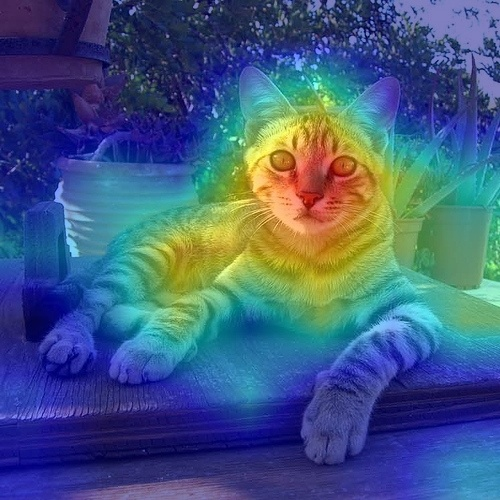
\includegraphics[width=0.20\textwidth,height=0.20\textwidth]
      {figures/val_cams/ours/2007_003778_7}
      \\
      \textbf{Bicycle}
       & 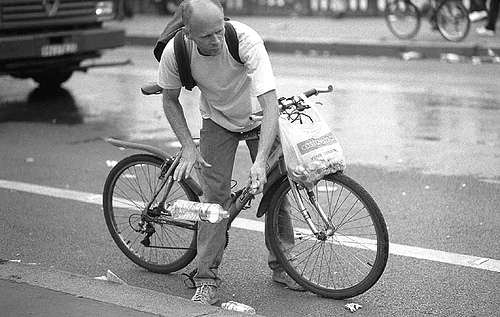
\includegraphics[width=0.20\textwidth,height=0.20\textwidth]
      {figures/originals/2011_000453}
       & 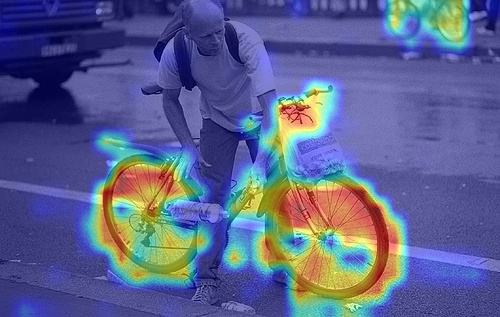
\includegraphics[width=0.20\textwidth,height=0.20\textwidth]
      {figures/val_cams/weclip/2011_000453_1}
       & 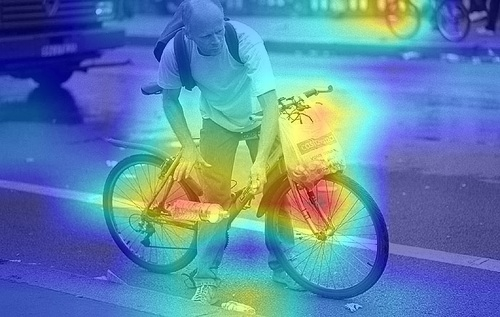
\includegraphics[width=0.20\textwidth,height=0.20\textwidth]
      {figures/val_cams/ours/2011_000453_1}
      \\
      \textbf{Bird}
       & 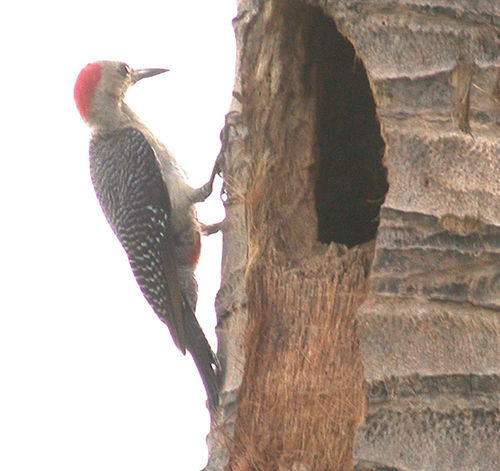
\includegraphics[width=0.20\textwidth,height=0.20\textwidth]
      {figures/originals/2011_001902}
       & 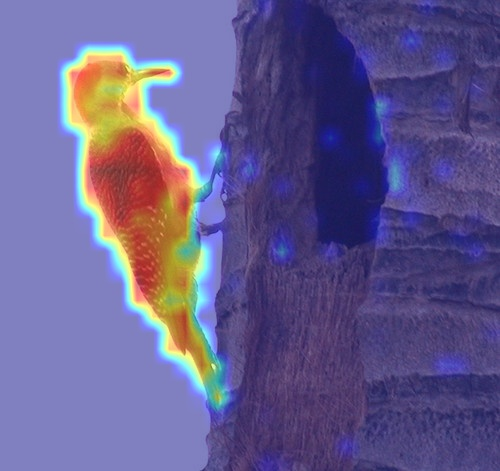
\includegraphics[width=0.20\textwidth,height=0.20\textwidth]
      {figures/val_cams/weclip/2011_001902_2}
       & 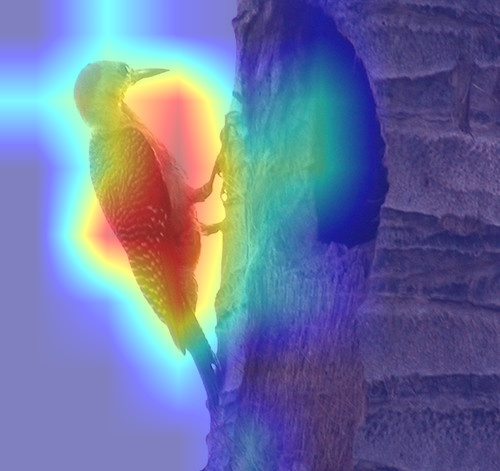
\includegraphics[width=0.20\textwidth,height=0.20\textwidth]
      {figures/val_cams/ours/2011_001902_2}
      \\
      \textbf{Boat}
       & 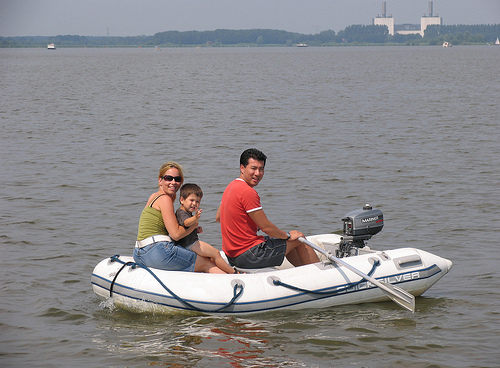
\includegraphics[width=0.20\textwidth,height=0.20\textwidth]
      {figures/originals/2010_003599}
       & 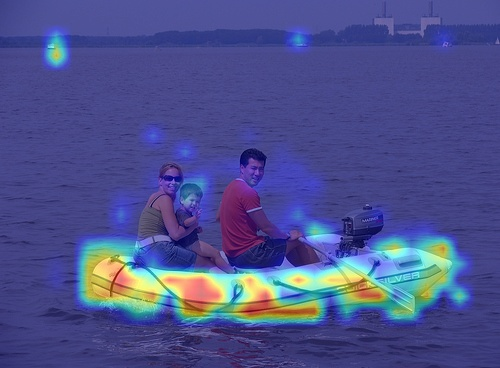
\includegraphics[width=0.20\textwidth,height=0.20\textwidth]
      {figures/val_cams/weclip/2010_003599_3}
       & 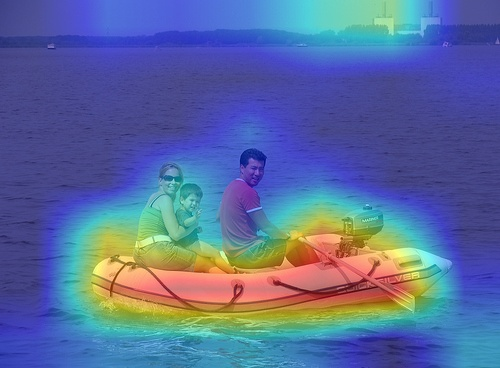
\includegraphics[width=0.20\textwidth,height=0.20\textwidth]
      {figures/val_cams/ours/2010_003599_3}
      \\
      \textbf{Pottedplant}
       & 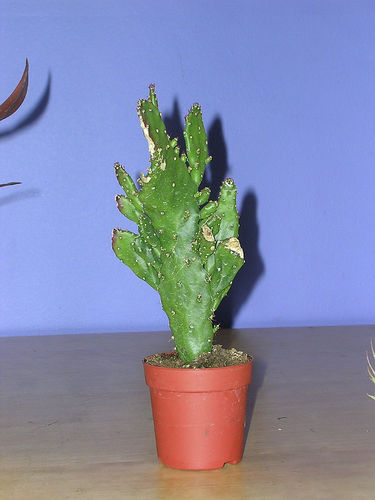
\includegraphics[width=0.20\textwidth,height=0.20\textwidth]
      {figures/originals/2011_000145}
       & 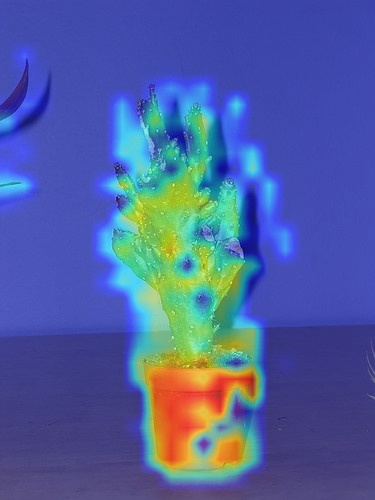
\includegraphics[width=0.20\textwidth,height=0.20\textwidth]
      {figures/val_cams/weclip/2011_000145_15}
       & 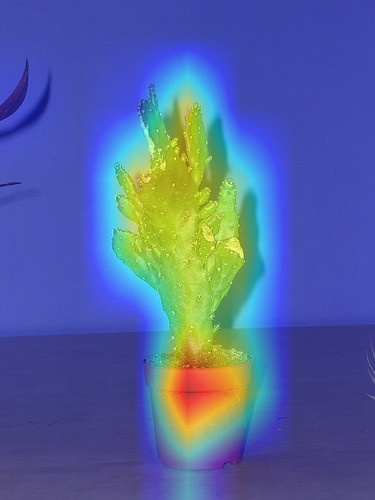
\includegraphics[width=0.20\textwidth,height=0.20\textwidth]
      {figures/val_cams/ours/2011_000145_15}
      \\
      \textbf{Car}
       & 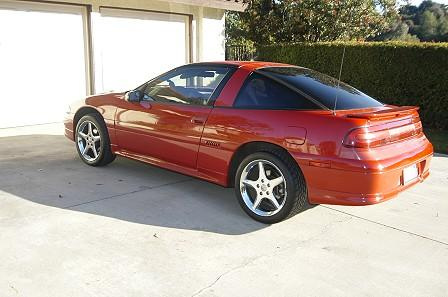
\includegraphics[width=0.20\textwidth,height=0.20\textwidth]
      {figures/originals/2010_005119}
       & 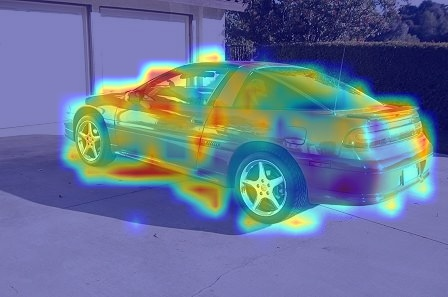
\includegraphics[width=0.20\textwidth,height=0.20\textwidth]
      {figures/val_cams/weclip/2010_005119_6}
       & 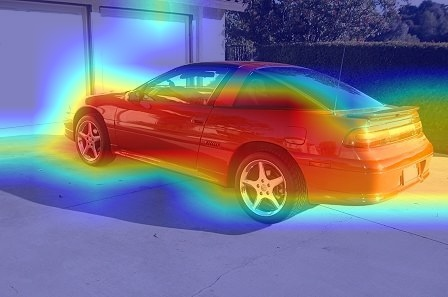
\includegraphics[width=0.20\textwidth,height=0.20\textwidth]
      {figures/val_cams/ours/2010_005119_6}
      \\
      \textbf{Bus}
       & 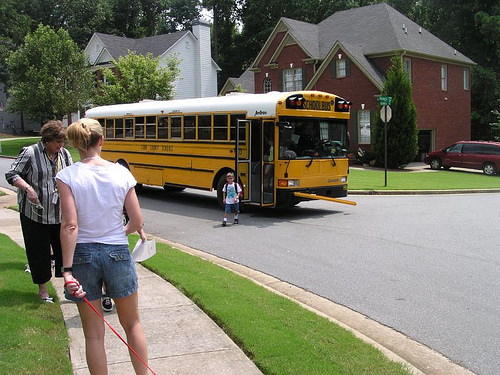
\includegraphics[width=0.20\textwidth,height=0.20\textwidth]
      {figures/originals/2010_000148}
       & 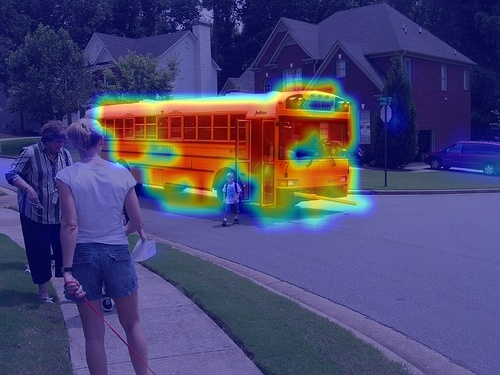
\includegraphics[width=0.20\textwidth,height=0.20\textwidth]
      {figures/val_cams/weclip/2010_000148_5}
       & 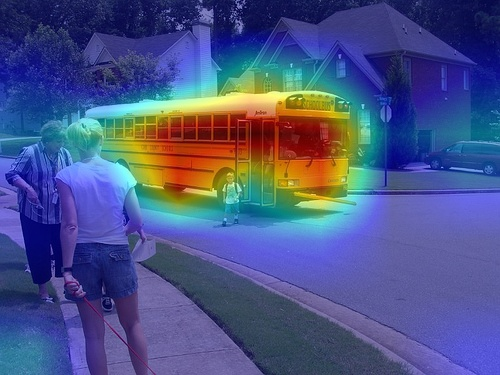
\includegraphics[width=0.20\textwidth,height=0.20\textwidth]
      {figures/val_cams/ours/2010_000148_5}
      \\
    \end{tabular}
  \end{tcolorbox}

  \caption{Qualitative comparison of CAMs between WeCLIP and our UniCL-AffSeg on PASCAL VOC 2012 \textit{val} set.}
  \label{fig:qualitative_comparison_cam_val}
\end{figure}


\begin{figure}[ht]
  \centering
  \setlength{\tabcolsep}{2pt} % adjust spacing
  \renewcommand{\arraystretch}{0.9}
  % Wrap the table in a colored box (requires \usepackage{tcolorbox})
  \begin{tcolorbox}[colframe=black!60, colback=white, boxrule=0.8pt, arc=2pt, left=2pt, right=2pt, top=2pt, bottom=2pt]
    \centering
    \begin{tabular}{cccc}
      (a) Input & (b) GT & (c) WeCLIP & (d) Ours           \\
      [1mm]

      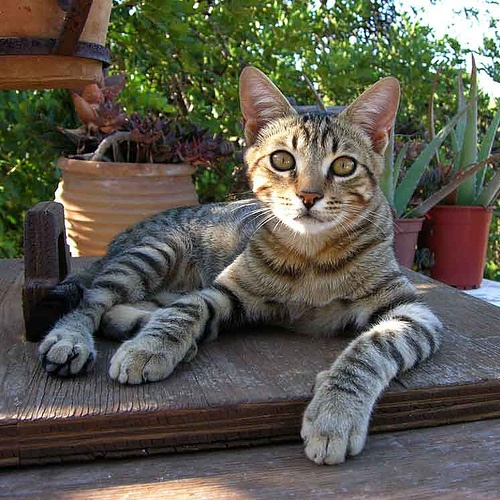
\includegraphics[width=0.20\textwidth,height=0.20\textwidth]
      {figures/originals/2007_003778}
                &
      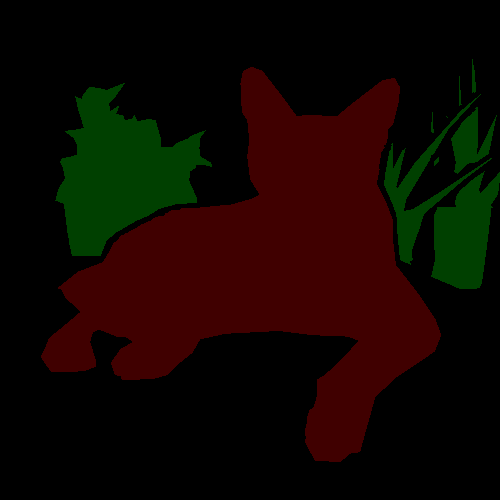
\includegraphics[width=0.20\textwidth,height=0.20\textwidth]
      {figures/colored_gts/2007_003778}
                &
      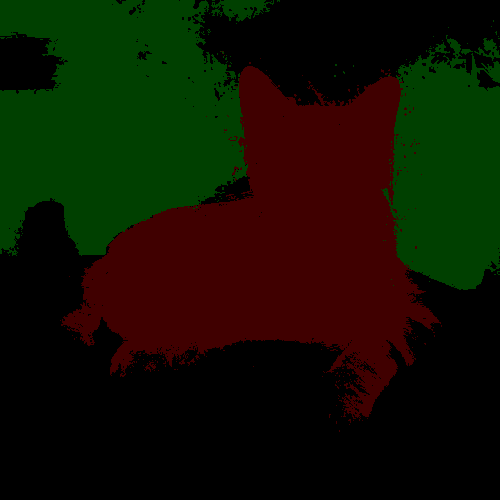
\includegraphics[width=0.20\textwidth,height=0.20\textwidth]
      {figures/val_labels/weclip/2007_003778_[7, 15]}
                &
      \includegraphics[width=0.20\textwidth,height=0.20\textwidth]
      {figures/val_labels/ours/2007_003778_[7, 15]}    \\

      \includegraphics[width=0.20\textwidth,height=0.20\textwidth]
      {figures/originals/2009_003768}
                &
      \includegraphics[width=0.20\textwidth,height=0.20\textwidth]
      {figures/colored_gts/2009_003768}
                &
      \includegraphics[width=0.20\textwidth,height=0.20\textwidth]
      {figures/val_labels/weclip/2009_003768_[12, 14]}
                &
      \includegraphics[width=0.20\textwidth,height=0.20\textwidth]
      {figures/val_labels/ours/2009_003768_[12, 14]}   \\

      \includegraphics[width=0.20\textwidth,height=0.20\textwidth]
      {figures/originals/2011_001967}
                &
      \includegraphics[width=0.20\textwidth,height=0.20\textwidth]
      {figures/colored_gts/2011_001967}
                &
      \includegraphics[width=0.20\textwidth,height=0.20\textwidth]
      {figures/val_labels/weclip/2011_001967_[2]}
                &
      \includegraphics[width=0.20\textwidth,height=0.20\textwidth]
      {figures/val_labels/ours/2011_001967_[2]}        \\


      \includegraphics[width=0.20\textwidth,height=0.20\textwidth]
      {figures/originals/2007_000250}
                &
      \includegraphics[width=0.20\textwidth,height=0.20\textwidth]
      {figures/colored_gts/2007_000250}
                &
      \includegraphics[width=0.20\textwidth,height=0.20\textwidth]
      {figures/val_labels/weclip/2007_000250_[4, 10]}
                &
      \includegraphics[width=0.20\textwidth,height=0.20\textwidth]
      {figures/val_labels/ours/2007_000250_[4, 10]}    \\


      \includegraphics[width=0.20\textwidth,height=0.20\textwidth]
      {figures/originals/2010_005119}
                &
      \includegraphics[width=0.20\textwidth,height=0.20\textwidth]
      {figures/colored_gts/2010_005119}
                &
      \includegraphics[width=0.20\textwidth,height=0.20\textwidth]
      {figures/val_labels/weclip/2010_005119_[6]}
                &
      \includegraphics[width=0.20\textwidth,height=0.20\textwidth]
      {figures/val_labels/ours/2010_005119_[6]}        \\



      \includegraphics[width=0.20\textwidth,height=0.20\textwidth]
      {figures/originals/2011_000453}
                &
      \includegraphics[width=0.20\textwidth,height=0.20\textwidth]
      {figures/colored_gts/2011_000453}
                &
      \includegraphics[width=0.20\textwidth,height=0.20\textwidth]
      {figures/val_labels/weclip/2011_000453_[1, 4, 14]}
                &
      \includegraphics[width=0.20\textwidth,height=0.20\textwidth]
      {figures/val_labels/ours/2011_000453_[1, 4, 14]} \\
    \end{tabular}

    \caption{Qualitative comparison of pseudo-labels between WeCLIP and our UniCL-AffSeg on PASCAL VOC 2012 \textit{val} set.}
    \label{fig:qualitative_comparison_pseudolabel_val}
  \end{tcolorbox}
\end{figure}


\begin{figure}[ht]
  \centering
  \setlength{\tabcolsep}{2pt} % adjust spacing
  \renewcommand{\arraystretch}{0.9}
  % Wrap the table in a colored box (requires \usepackage{tcolorbox})
  \begin{tcolorbox}[colframe=black!60, colback=white, boxrule=0.8pt, arc=2pt, left=2pt, right=2pt, top=2pt, bottom=2pt]
    \centering
    \begin{tabular}{cccc}
      (a) Input & (b) GT & (c) WeCLIP & (d) (Ours)           \\
      [1mm]

      \includegraphics[width=0.20\textwidth,height=0.20\textwidth]
      {figures/originals/2007_005331}
                &
      \includegraphics[width=0.20\textwidth,height=0.20\textwidth]
      {figures/colored_gts/2007_005331}
                &
      \includegraphics[width=0.20\textwidth,height=0.20\textwidth]
      {figures/test_labels/weclip/2007_005331_[6, 12, 14]}
                &
      \includegraphics[width=0.20\textwidth,height=0.20\textwidth]
      {figures/test_labels/ours/2007_005331_[6, 12, 14]}    \\

      \includegraphics[width=0.20\textwidth,height=0.20\textwidth]
      {figures/originals/2007_006277}
                &
      \includegraphics[width=0.20\textwidth,height=0.20\textwidth]
      {figures/colored_gts/2007_006277}
                &
      \includegraphics[width=0.20\textwidth,height=0.20\textwidth]
      {figures/test_labels/weclip/2007_006277_[6]}
                &
      \includegraphics[width=0.20\textwidth,height=0.20\textwidth]
      {figures/test_labels/ours/2007_006277_[6]}   \\

      \includegraphics[width=0.20\textwidth,height=0.20\textwidth]
      {figures/originals/2008_001504}
                &
      \includegraphics[width=0.20\textwidth,height=0.20\textwidth]
      {figures/colored_gts/2008_001504}
                &
      \includegraphics[width=0.20\textwidth,height=0.20\textwidth]
      {figures/test_labels/weclip/2008_001504_[14]}
                &
      \includegraphics[width=0.20\textwidth,height=0.20\textwidth]
      {{figures/test_labels/ours/2008_001504_[14]}}        \\


      \includegraphics[width=0.20\textwidth,height=0.20\textwidth]
            {figures/originals/2008_002358}
                &
      \includegraphics[width=0.20\textwidth,height=0.20\textwidth]
      {figures/colored_gts/2008_002358}
                &
      \includegraphics[width=0.20\textwidth,height=0.20\textwidth]
      {figures/test_labels/weclip/2008_002358_[0]}
                &
      \includegraphics[width=0.20\textwidth,height=0.20\textwidth]
      {figures/test_labels/ours/2008_002358_[0]}    \\


      \includegraphics[width=0.20\textwidth,height=0.20\textwidth]
      {figures/originals/2009_003224}
                &
      \includegraphics[width=0.20\textwidth,height=0.20\textwidth]
      {figures/colored_gts/2009_003224}
                &
      \includegraphics[width=0.20\textwidth,height=0.20\textwidth]
      {figures/test_labels/weclip/2009_003224_[1]}
                &
      \includegraphics[width=0.20\textwidth,height=0.20\textwidth]
      {figures/test_labels/ours/2009_003224_[1]}        \\



      \includegraphics[width=0.20\textwidth,height=0.20\textwidth]
      {figures/originals/2009_004084}
                &
      \includegraphics[width=0.20\textwidth,height=0.20\textwidth]
      {figures/colored_gts/2009_004084}
                &
      \includegraphics[width=0.20\textwidth,height=0.20\textwidth]
      {figures/test_labels/weclip/2009_004084_[2]}
                &
      \includegraphics[width=0.20\textwidth,height=0.20\textwidth]
      {figures/test_labels/ours/2009_004084_[2]} \\

      
      \includegraphics[width=0.20\textwidth,height=0.20\textwidth]
      {figures/originals/2010_002531}
                &
      \includegraphics[width=0.20\textwidth,height=0.20\textwidth]
      {figures/colored_gts/2010_002531}
                &
      \includegraphics[width=0.20\textwidth,height=0.20\textwidth]
      {figures/test_labels/weclip/2010_002531_[7, 17]}
                &
      \includegraphics[width=0.20\textwidth,height=0.20\textwidth]
      {figures/test_labels/ours/2010_002531_[7, 17]} \\


    \end{tabular}

    \caption{Qualitative comparison of pseudo-labels between WeCLIP and our UniCL-AffSeg on PASCAL VOC 2012 \textit{test} set.}
    \label{fig:qualitative_comparison_pseudolabel_test}
  \end{tcolorbox}
\end{figure}


\subsection{Observations}

\subsubsection{Class Activation Maps (CAMs)}
Our UniCL-AffSeg CAMs demonstrate superior performance compared to WeCLIP in several key aspects:
\begin{itemize}
    \item \textbf{Enhanced Object Coverage and Completeness}: UniCL-AffSeg CAMs exhibit more contiguous and complete activation regions. For instance, in images such as \texttt{2007\_003778\_7.jpg} (cat) and \texttt{2011\_000453\_1.jpg} (bicycle), our CAMs capture larger, more holistic object areas, reducing sparsity and better approximating full object extents. This is attributed to the Swin-based affinity refinement, which effectively propagates activations across object parts.
    \item \textbf{Reduced Background Noise and Sharper Boundaries}: WeCLIP CAMs often include extraneous background activations, leading to noisy and diffuse maps (e.g., in \texttt{2010\_005119\_6.jpg} for car and \texttt{2010\_000148\_5.jpg} for bus). In contrast, UniCL-AffSeg CAMs show cleaner, more focused activations with sharper edges, minimizing false positives. This highlights the benefits of multi-modal fusion in UniCL over WeCLIP's ViT-only approach.
    \item \textbf{Improved Handling of Complex or Small Objects}: For challenging cases like \texttt{2011\_000145\_15.jpg} (pottedplant) and \texttt{2010\_003599\_3.jpg} (boat), UniCL-AffSeg CAMs provide finer granularity and better localization, capturing subtle details that WeCLIP misses. This is evident in multi-class images (e.g., \texttt{2007\_005702\_1.jpg}), where our method separates classes more effectively.
    \item \textbf{Consistency Across Datasets}: These improvements are consistent across both validation and test sets, with examples like \texttt{2007\_005331\_[6, 12, 14].jpg} demonstrating robustness in cluttered scenes.
\end{itemize}

\subsubsection{Pseudo-Labels}
The pseudo-labels generated by UniCL-AffSeg show marked improvements over WeCLIP, aligning more closely with ground truth annotations:
\begin{itemize}
    \item \textbf{Higher Mask Accuracy}: UniCL-AffSeg pseudo-labels capture object shapes more precisely, with fewer misclassifications or holes. For example, in \texttt{2007\_003778\_[7, 15].png} (cat and person), our masks outperform WeCLIP's fragmented outputs.
    \item \textbf{Finer Boundary Delineation}: Our pseudo-labels exhibit cleaner, more defined edges, reducing noise and over-segmentation. In test examples like \texttt{2008\_001504\_[14].png} (horse) and \texttt{2009\_003224\_[1].png}, WeCLIP produces noisy masks, while UniCL-AffSeg yields smoother, more accurate boundaries.
    \item \textbf{Better Performance on Diverse Scenarios}: Trends hold for easy (e.g., \texttt{2011\_001967\_[2].png} for bird) and hard cases (e.g., \texttt{2010\_005119\_[6].png} for car), with UniCL-AffSeg narrowing the gap to fully supervised methods. Limitations persist for highly occluded or tiny objects (e.g., \texttt{2007\_000250\_[4, 10].png}).
    \item \textbf{Cross-Set Generalization}: Similar gains are observed in test labels, such as \texttt{2009\_004084\_[2].png}, underscoring boundary precision and completeness.
\end{itemize}

Overall, these qualitative results underscore UniCL-AffSeg's advantages in weakly supervised semantic segmentation, driven by its Swin transformer backbone and affinity-based refinement. This supports the quantitative improvements (e.g., higher mIoU) reported in the results section, demonstrating UniCL-AffSeg's potential to bridge the gap with fully supervised approaches.





\subsection{Per-Class Performance Analysis}
\label{subsec:per_class_performance_analysis}

To gain a deeper understanding of our model’s behavior, we analyzed the per-class Intersection over Union (IoU) scores on the PASCAL VOC 2012 validation set. This analysis highlights how the model performs across different object categories, providing insights beyond the overall metrics.

\subsubsection{High-Performing Classes}

Classes with a large spatial extent and higher representation in the dataset achieve relatively high IoU scores. For instance, \textbf{background} (77.8\%), \textbf{bus} (67.5\%), \textbf{cat} (65.9\%), and \textbf{dog} (65.1\%) are segmented effectively. These results indicate that the model can reliably capture dominant objects with distinctive visual features.

\subsubsection{Low-Performing Classes}

In contrast, smaller or less frequent classes such as \textbf{person} (16.9\%), \textbf{chair} (25.3\%), and \textbf{potted plant} (28.3\%) exhibit lower IoU scores. This suggests that the model struggles with rare or small objects, likely due to their limited representation in the training set and small spatial footprint in the images.

\subsubsection{Observations}

Overall, the model performs better on large and visually distinctive classes such as animals and vehicles, while it underperforms on humans, furniture, and small objects. These per-class performance results provide valuable insights that can guide future improvements, such as incorporating multi-scale features or class-specific data augmentation to better handle challenging classes.


\begin{table}[ht]
\centering
\caption{Per-Class IoU Performance on PASCAL VOC (Latest Results)}
\begin{tabular}{|c|l|c|}
\hline
\textbf{Index} & \textbf{Class}      & \textbf{IoU} \\ \hline
0  & background   & 0.7784  \\
1  & aeroplane    & 0.5685  \\
2  & bicycle      & 0.3191  \\
3  & bird         & 0.6044  \\
4  & boat         & 0.4360  \\
5  & bottle       & 0.3677  \\
6  & bus          & 0.6753  \\
7  & car          & 0.4881  \\
8  & cat          & 0.6591  \\
9  & chair        & 0.2525  \\
10 & cow          & 0.5887  \\
11 & diningtable  & 0.4041  \\
12 & dog          & 0.6511  \\
13 & horse        & 0.6132  \\
14 & motorbike    & 0.5846  \\
15 & person       & 0.1697  \\
16 & pottedplant  & 0.2828  \\
17 & sheep        & 0.6305  \\
18 & sofa         & 0.4661  \\
19 & train        & 0.5642  \\
20 & tvmonitor    & 0.4032  \\ \hline
\end{tabular}
\end{table}

\begin{table}[ht]
\centering
\caption{Overall Performance Metrics}
\begin{tabular}{|l|c|}
\hline
\textbf{Metric} & \textbf{Value} \\ \hline
Pixel Accuracy (pAcc) & 0.7981 \\
Mean Accuracy (mAcc)  & 0.6997 \\
Mean IoU (mIoU)       & 0.5003 \\ \hline
\end{tabular}
\end{table}

% The model achieved a mean IoU of 0.5003 on the PASCAL VOC dataset, with a pixel accuracy of 0.7981 and a mean accuracy of 0.6997. Performance varies significantly across classes: large and well-represented classes such as \textbf{background} (0.7784), \textbf{bus} (0.6753), \textbf{cat} (0.6591), and \textbf{dog} (0.6511) are segmented effectively, while smaller or less frequent classes like \textbf{person} (0.1697), \textbf{chair} (0.2525), and \textbf{potted plant} (0.2828) remain challenging. These results suggest that while the model captures the dominant classes well, further improvements are needed to better handle rare and small objects.
\section{Ablation Study}
\label{sec:ablation_study}
\begin{table}[h!]
\centering
\begin{tabular}{|l|c|}
\hline
\textbf{Class} & \textbf{IoU} \\
\hline
background    & 0.79597609 \\
aeroplane     & 0.60649828 \\
bicycle       & 0.24300995 \\
bird          & 0.56525227 \\
boat          & 0.41434259 \\
bottle        & 0.39108619 \\
bus           & 0.63887711 \\
car           & 0.41678079 \\
cat           & 0.52468153 \\
chair         & 0.24156961 \\
cow           & 0.57364590 \\
diningtable   & 0.31857660 \\
dog           & 0.56249454 \\
horse         & 0.56194598 \\
motorbike     & 0.53527557 \\
person        & 0.21941806 \\
potted plant  & 0.28315749 \\
sheep         & 0.59557354 \\
sofa          & 0.37300971 \\
train         & 0.53391481 \\
tv/monitor    & 0.45051146 \\
\hline
\textbf{Mean IoU (mIoU)} & \textbf{0.46883800} \\
\hline
\end{tabular}
\caption{Per-class IoU and mIoU for Pascal VOC without RFM.}
\label{tab:pascal_first_set_miou}
\end{table}



\input{chapters/Discussion/discussion.tex}
% \chapter{Conclusion}
% \label{chap:conclusion}

% % Semantic segmentation remains a core challenge in computer vision, requiring pixel-level understanding of images to support applications ranging from autonomous driving to medical imaging. While fully supervised approaches have achieved impressive results, they come with the heavy burden of requiring vast amounts of finely annotated data. Weakly Supervised Semantic Segmentation (WSSS) presents a promising alternative by dramatically reducing this annotation effort, relying instead on weaker forms of supervision such as image-level labels. However, the success of WSSS critically depends on the quality of Class Activation Maps (CAMs), which are used to generate pseudo-labels for training segmentation models.

% % In this thesis, we addressed the core limitations of existing WSSS pipelines: the generation of incomplete, sparse, and coarse CAMs. Recognizing that a backbone's ability to capture both local and global contexts significantly influences CAM quality, we systematically explored stronger backbone architectures to generate better CAMs. Our work did not restrict itself to any single model; instead, we focused on understanding how models such as UniCL and Swin Transformer, with their multi-modal and hierarchical characteristics, could enhance CAM generation. We demonstrated that backbones capable of capturing fine-grained local details along with broader global semantics produce richer and more complete activation maps.

% % Beyond backbone selection, we studied and experimented on an enhanced CAM refinement strategy. We have combined the strengths of both affinity-based and pixel-wise refinement methods to create a more robust pipeline. But after training we have our results to be very poor. The reason we have identified is that the process aggregating the intermediate features from the UniCL backbone, which were non-uniform in shapes, was not properly handled. Also, for the same reason, the pixel-wise refinement did not work properly. But we have shown that UniCL is a very strong backbone and we have shown that it can localize the objects very well and the CAMs are significantly good. We need to further investigate the affinity-based refinement strategy and how to properly aggregate the features from the backbone. We also need to investigate how to properly use the pixel-wise refinement strategy. 

% % The importance of this research lies not only in the immediate improvements observed in segmentation results but also in the broader implications for future WSSS systems. By showing that careful selection of backbones and effective affinity-based refinement strategies can close the gap between weakly and fully supervised methods, we offer a viable path toward scalable, annotation-efficient semantic segmentation. Our findings encourage further research into leveraging the rich affinity information inherently captured by advanced architectures and suggest that even stronger results are possible with newer, self-supervised, or multi-modal vision models.

% % In conclusion, this thesis highlights that improving the initial CAM quality and designing robust refinement pipelines are pivotal to advancing WSSS performance. 

% \chapter{Citations}
\label{chap:citations}

% Before the references section
\begingroup
\tolerance=2000 % Relax the tolerance for line breaking
\emergencystretch=0pt % Reset the emergency stretch
\hyphenpenalty=50 % Allow hyphenation with a lower penalty
\hbadness=2000 % Allow some warnings about underfull or overfull lines


\printbib

% % End of the relaxed settings
\endgroup



\end{document}
